% 202? - Francisco Fernandez tesis template
%
% https://github.com/fernandezfran/tesis
\documentclass[12pt,spanish,a4paper,twoside]{book}
\usepackage[spanish,es-nodecimaldot]{babel}

% colores nord blues
\usepackage{xcolor}
\definecolor{mycolor}{RGB}{94, 129, 172} % nord blue
\definecolor{mylcolor}{RGB}{129, 161, 193} % nord lighter blue

% estilo de pagina
%
%% margenes
\usepackage{geometry}
\geometry{
	a4paper,
	total={170mm,257mm},
	left=20mm,
	top=20mm,
}
%
%% Sangría
\setlength\parindent{12pt}
%
%% Interlineado
\usepackage{setspace}
\onehalfspacing
%
%% Palatino font type
\usepackage[T1]{fontenc}
\usepackage{mathpazo}
%
%% poder definir margenes de un parrafo (adjustwidth)
\usepackage{changepage}
%% encabezados de las páginas
\usepackage{fancyhdr}
\pagestyle{fancy}
\fancyhf{}
%
%%% línea horizontal superior
\let\oldheadrule\headrule
\renewcommand{\headrule}{\color{mycolor}\oldheadrule}
\renewcommand{\headrulewidth}{0.8pt}
%
%%% línea horizonal inferior
%\let\oldfootrule\footrule
%\renewcommand{\footrule}{\color{mycolor}\oldfootrule}
%\renewcommand{\footrulewidth}{0.8pt}
%
%%% header
\renewcommand{\chaptermark}[1]{\markboth{#1}{}}
\renewcommand{\sectionmark}[1]{\markright{#1}}
\fancyhead[CE]{\footnotesize\color{mycolor}\normalfont\bfseries\itshape\nouppercase{
    \textsc{\leftmark}}
}
\fancyhead[CO]{\footnotesize\color{mycolor}\normalfont\bfseries\itshape\nouppercase{
    \textsc{\rightmark}}
}
%
%%% footer
\fancyfoot[CE,CO]{\color{mycolor}\bfseries\thepage}
%
%% carátula de capítulo
\usepackage{sectsty}
\usepackage{titlesec}
\titleformat{\chapter}
    [display]
    {\centering\Huge\bfseries\color{mycolor}}
    {\chaptername\ \thechapter}
    {0pt}
    {\huge}
%
%% color de las secciones
\sectionfont{\color{mycolor}}
\subsectionfont{\color{mycolor}}
\subsubsectionfont{\color{mycolor}}
\let\oldtextbf\textbf
\renewcommand{\textbf}[1]{\textcolor{mycolor}{\oldtextbf{#1}}}
%
%% línea horizontal debajo de las secciones
\titleformat{\section}
  {\normalfont\Large\bfseries\color{mycolor}}
  {\thesection}{1em}{}[{\titlerule[0.8pt]}]
%
%% index
\usepackage{imakeidx}
\makeindex[columns=3, title=Alphabetical Index, intoc]
%
%% show subsubsections in TOC
\setcounter{tocdepth}{4}
\setcounter{secnumdepth}{4}
%
%% Bibliografía por capítulo
% \usepackage[square,numbers,sort,sectionbib]{natbib}
% \usepackage{chapterbib}
%
%% defino pagina en blanco
\newcommand\blankpage{%
    \null
    \thispagestyle{empty}%
    \addtocounter{page}{-1}%
    \newpage
}

% para, desde el índice, poder clickear a que página ir
%\usepackage[obeyspaces]{url}
\usepackage[breaklinks=true,hidelinks]{hyperref} 

% \say para las comillas
\usepackage{dirtytalk}

% para agregar imagenes (includegraphics)
\usepackage{graphicx}
% espeficicando el path imagenes/ que se repetiría en todas las entradas
\graphicspath{{src/imagenes/}}
% subfiguras, definidas en columnas, por ej
\usepackage{subcaption}

% tabla en vez de cuadro
\usepackage[tableposition=top]{caption}
\addto\captionsspanish{
    \def\listtablename{\'Indice de tablas}%
    \def\tablename{Tabla}
}
%
%% para poder separar los títulos en dos renglones
\usepackage{adjustbox}\usepackage{mathtools}
\usepackage{array}
\usepackage{makecell,booktabs}
\usepackage{stackengine}
\setstackEOL{\cr} %EOL is abbreviation for "end of line."

% para acomodar mejor las posiciones de figuras/tablas
\usepackage{float}

% para algunos símbolos en las ecuaciones
\usepackage{amsmath}
\usepackage{mathtools}  % cases




\begin{document}

% enumeración de las primeras páginas con números romanos
\frontmatter

\blankpage
\blankpage

% Carátula
\thispagestyle{empty}
\begin{center}
{\large

    \vspace{1cm}

    {\Huge Simulaciones computacionales para el desarrollo de electrodos de 
            baterias de ion-litio de próxima generación}
    
    \vspace{0.5cm}
    por
    \vspace{0.5cm}
    
    {\Large Francisco Fernandez}

    \vspace{0.5cm}

    Presentado ante la Facultad de Matemáticas, Astronomía, Física y Computación 
    como parte de los requerimientos para la obtención del grado de
    
    \vspace{0.5cm}

    {\Large Doctor en Física}

    \vspace{0.5cm}
    de la

    UNIVERSIDAD NACIONAL DE CÓRDOBA

    \vspace{0.5cm}
    % logo 
    
    mes, 202?

    \textcopyright FaMAF - UNC 202?

    \vspace{1.5cm}

    Director: Daniel Eugenio Barraco Díaz

    Codirector: Ezequiel Pedro Marcos Leiva

    % licencia
}
\end{center}

% Dedicatoria

% Índice
\tableofcontents
\listoffigures
% \listoftables

% Resumen

% Abstract

% a partir de acá se cuentan los números de las páginas en formato arabico
\mainmatter

% Capítulos...

\chapter[Introducción]{Introducción}
\thispagestyle{empty}

\clearpage
\newpage
\thispagestyle{empty}
\mbox{}
\newpage

El calentamiento global es el mayor problema ambiental que enfrenta el mundo, el 
mismo se refiere al efecto que producen las actividades humanas en el clima, como 
la quema de combustibles fósiles o la deforestación, que emiten a la atmósfera
grandes cantidades de dióxido de carbono, CO$_2$, entre otros gases de efecto 
invernadero. Estos gases absorben la radiación infrarroja emitida por la tierra 
provocando un incremento de la temperatura de la misma que lleva asociado un 
aumento en la frecuencia y la intensidad de eventos climáticos extremos 
~\cite{houghton2005}. Según el Panel Intergubernamental del Cambio Climático 
(IPCC), desde la época preindustrial, las actividades humanas han provocado 
aproximadamente 1.0$^{\circ}$C de calentamiento global y al ritmo actual se van 
a sobrepasar los 1.5$^{\circ}$C antes del 2050, un cambio en la temperatura
media que las emisiones previas por sí solas no habían alcanzado
~\cite{harvey2018}. Limitar el calentamiento a esta temperatura requiere que se 
realicen rápidamente cambios sin precedentes en la tecnología y en el 
comportamiento humano. Uno de los cambios más importante es el de la matriz 
energética, en la cual las energías renovables deberán suministrar alrededor del 
80\% de la energía para 2050, donde los vectores energéticos, como las baterías 
de litio, juegan un rol fundamental debido a la intermitencia de estas formas de 
generación de energía.

El litio es el metal más liviano de la tabla periódica y uno de los elementos más
importantes dentro de los minerales necesarios en la producción de baterías de
litio. En particular, para la Argentina tiene un interés económico, social, 
industrial y tecnológico ya que es uno de los países que integran, junto a 
Bolivia y Chile, el Triangulo de Litio, el cual acumula el 70\% de las reservas 
mundiales de este mineral. Aún más importante que esta cantidad de reservas es 
que las mismas se encuentran en salares que, a grandes rasgos, es más barato
extraer litio de ellos en comparación a las pegmatitas, heroctitas o jadaritas, 
que son las rocas de las cuales se puede extraer litio en una minería usual.
A pesar de esto se tienen que llevar a cabo distintas consideraciones ambientales,
sociales y legales del proceso de extracción e incentivar el desarrollo de valor
agregado a dicha extracción ~\cite{heredia2020}.

En esta tesis se presentan estudios realizados mediante el uso de simulaciones 
computacionales en... TODO


\section{Transición energética}

La demanda internacional de energía sigue en aumento debido al crecimiento 
poblacional rápido y a los avances en la civilización, más del 80\% de la misma
sigue siendo producida por combustibles fósiles, que son limitados en recursos 
y tienen un impacto grave en el medio ambiente. Sin políticas comprometidas con 
la transición energética no se espera que esta proporción disminuya, dejando 
lugar a la producción de energía mediante fuentes renovables, en los próximos 20
años. Si el cambio en la matriz energética se deja en manos del mercado, las 
fuentes de energía limpias no sustituirán por sí solas a los métodos tradicionales
hasta que no sólo alcancen una paridad de precios, si no que se vuelvan 
considerablemente más baratas de manera que justifiquen dicho cambio
~\cite{davidson2019}. Dicho esto, cumplir los objetivos climáticos y realizar la 
transición hacia un futuro con menos carbono va a requerir inversiones 
sustanciales por parte de los gobiernos ~\cite{leonhardt2022}.

La gran mayoría de las naciones desarrolladas han implementado un marco legal de 
apoyo y habilitación para ayudar a promover la integración de las energías 
renovables modernas en sus sistemas energéticos. Estas políticas se han 
desarrollado como resultado, o en apoyo, de acuerdos internacionales como el 
Acuerdo de París, el Protocolo de Kioto o el Green Deal europeo. Los objetivos 
de las energías renovables y los incentivos fiscales dirigidos al sector 
energético son las dos políticas más comunes en países en desarrollo para apoyar 
la transición energética ~\cite{cantarero2020}.

En Argentina el sector energético depende altamente de la utilización de 
combustibles fósiles, donde la capacidad de generación de energía está 
principalmente atada a las centrales térmicas convencionales y a grandes 
centrales hidroeléctricas, mientras que tan sólo una pequeña cantidad proviene 
de plantas nucleares y de fuentes de energías renovables. En cuanto al potencial
de producción de energía de fuentes renovables, Argentina tiene una gran 
capacidad eólica y solar. El gobierno nacional viene incentivando la instalación 
de dichas fuentes de energía desde 2009, mediante el programa GENREN. A fines 
del 2015 se estableció un objetivo de que el 20\% de la energía fuera generada
mediante estas fuentes para 2025 y en 2016 se introdujo un nuevo esquema de 
compra con el programa RenovAr ~\cite{schaube2018}. Este desarrollo viene 
acompañado de un amplio espectro de investigaciones académicas 
interdisciplinarias.

\subsection{Energías renovables}

Existen muchas formas de generación de energías renovables, entre ellas destacan:
\begin{itemize}
    \item la \textbf{biomasa}, que permite obtener la energía química 
        que se encuentra almacenada en la materia orgánica mediante la quema de 
        la misma,
    \item la \textbf{hidráulica}, que aprovecha la energía cinética y potencial
        de la corriente del agua, la \textbf{marina}, transportada en las olas
        del mar,
    \item la \textbf{eólica}, obtenida a partir de la energía cinética del viento,
    \item la \textbf{solar}, que permite producir energía a partir de la radiación
        electromagnética del sol.
\end{itemize}
La producción de dispositivos eficientes de obtención de energía renovable es un 
requisito esencial para mejorar la eficiencia y, finalmente, reducir el costo de 
las fuentes de energía renovables. Este es uno de los retos a los que se 
enfrenta el establecimiento generalizado de las mismas en comparación con fuentes
de energía tradicionales ~\cite{olabi2022}. Para dar un ejemplo, la energía solar 
se encuentra disponible en todas partes y ya se aplica comercialmente en varios 
sectores. Uno de los principales retos a los que se enfrenta la misma es a los 
días nublados, que afecta negativamente a la producción de energía. La 
generalización de los sistemas solares fotovoltaicos requiere sistemas eficientes 
de almacenamiento de energía, donde las baterías son las más accesibles. 

\subsection{Sistemas de almacenamiento de energía}

Como una solución al problema de la alta intermitencia, la baja predictibilidad 
diaria y la variación estacional de energías renovables, se introducen sistemas 
de almacenamiento de energía. La energía de estas fuentes debe ser almacenada 
cuando están produciendo energía por demás y esta puede ser liberada cuando se 
requiera. Dichos sistemas pueden ser clasificados a grandes rasgos en mecánicos, 
electroquímicos, químicos o térmicos ~\cite{khan2019}.

En el caso de los sistemas de almacenamiento de energía mecánicos, la energía se
almacena realizando algún trabajo mecánico, entre ellos se encuentra, por ejemplo,
el aire comprimido. En el almacenamiento de energía térmica se utiliza la energía 
térmica que se produce al calentar o enfriar un medio.

En el sistema químico, la energía se almacena en forma de energía química 
almacenada en distintos materiales. Se tienen principalmente dos tipos, los
biocombustibles o el hidrógeno. En este último caso, la energía eléctrica se 
utiliza para descomponer el agua en oxígeno e hidrógeno, estos gases se almacenan 
y se transportan para luego volver a combinarse y liberar la energía almacenada.

Por último, dentro de los sistemas de almacenamiento de energía electroquímicos 
se encuentran las baterías y los capacitores. En las baterías, tanto a la entrada 
como la salida de energía la misma se encuentra en forma de energía eléctrica 
mientras que la electricidad se almacena en energía química. 


\section{Baterías}

TODO: Clasificación de baterías en primarias (no recargables) o secundarias 
(recargables). Funcionamiento de una batería, sus partes. Gráfico de densidad
de energía volumétrica vs densidad de energía gravimétrica.

La primera batería concebida fue inventada por Alessandro Volta en 1800 para 
estudiar los descubrimientos de Luigi Galvani, la misma basa su funcionamiento 
en la combinación de zinc con cobre y se la conoce como pila voltaica, fue 
crucial para los primeros experimentos electroquímicos. En 1866 la celda primaria 
de Leclanche, predecesora de la pila de zinc-carbono actual, se convirtió en una
de las primeras baterías comerciales al ser utilizada en estaciones de telegrafía
y en los primeros teléfonos. A mediados del siglo XIX surgió la necesidad de un 
sistema de almacenamiento recargable debido a la invención del generador 
eléctrico, la misma fue satisfecha por Gaston Panté al presentar la batería de 
plomo-ácido. Durante este último periodo de tiempo y principios del siglo XX, 
los motores de combustión interna y los motores eléctricos compitieron como medios
de propulsión en los automóviles. Con el descubrimiento de reservas de petróleo 
mayores a principios del siglo XX y el desarrollo de automóviles de gasolina más
cómodos, los vehículos eléctricos se vieron rápidamente superados por los de 
motores de combustión interna y se dejaron de fabricar. Por desgracia, el sector 
del transporte se convirtió en uno de los responsables de gran parte de la 
contaminación.

Un siglo después aparecieron nuevas iniciativas en el campo de las baterías con
el desarrollo del consumo de la electrónica portátil, que requiere una batería 
recargable de alta densidad energética que no es una condición que cumpla la 
batería de plomo-ácido. Inicialmente se prestó mucha atención al sistema 
níquel-cadmio hasta ser superado por las baterías de iones de litio (LIB) a 
principios de la década del 1990. Desde esa fecha, las LIB continúan mejorando
constantemente y prometen desempeñar un papel vital en el desarrollo de vehículos
eléctricos y el almacenamiento de energía de fuentes alternativas. % schipper2016

\subsection{Baterías de ion litio}

Las baterías de litio son dispositivos electroquímicos ampliamente utilizados 
como fuentes de energía. Entre las propiedades físicas del litio destacan su 
peso molecular bajo (7 g mol$^{-1}$), su densidad baja (0.534 cm$^3$), su 
capacidad específica alta (3860 mAh g$^{-1}$) y su potencial de reducción bajo 
(-3.04 V vs. SHE), estas propiedades lo convirtieron en un material que puede 
ser utilizado como ánodo para baterías. 

A finales de la década del 1950 se observó que el litio metálico formaba una capa 
de pasivación, llamada interfaz de electrolito sólido (SEI, de sus siglás en 
inglés, \textit{solid electrolyte interface}), con distintos electrolitos 
no-acuosos permitiendo prevenir una reacción química directa entre estas dos 
componentes, pero dejando que los iones de litio la atraviesen ~\cite{peled1979}. 
Esto generó un interés que llevó a la fabricación de baterías primarias de litio 
en la década del 1960 utilizando distintos tipos de cátodos incluyendo dióxido de 
sulfuro de litio (LiSO$_2$), óxido de manganeso de litio (LiMnO$_2$) y óxido de 
cobre de litio (LiCuO), entre otros. Desafortunadamente, la formación de la SEI 
no es estable durante ciclos prolongados y se agrieta, lo que lleva a un consumo 
continuo de electrolito y litio para la reformación continua de la SEI 
~\cite{besenhard1976}. Y lo que es aún peor, la deposición desigual de litio en 
la SEI agrietada conduce al crecimiento de dendritas de litio, que terminan 
rompiéndose y formando islas de tamaño nanométrico de litio altamente reactivo, 
lo que reduce la estabilidad térmica de la celda ~\cite{yamaki1998}. Las 
dendritas también pueden crecer lo suficiente como para generar un contacto 
entre el ánodo y el cátodo, provocando un cortocircuito. 

Avances posteriores en la comprensión de la intercalación de litio en diferentes
materiales dio origen a las baterías recargables de ion-litio. El primero de 
estos materiales fue utilizado por EXXON para una primera versión de las mismas.
Whittingham demostró en 1976 que el litio se intercala entre las capas que se 
forman en los metales de transición en una proporción de un mol que provoca una
expansión del parámetro de red ~\cite{whittingham1976}. El material más 
interesante de estos era el TiS$_2$, que ofrece el menor peso molecular, un costo 
potencialmente bajo y es un conductor eléctrico. Sin embargo, esta batería seguía
utilizando litio metálico como ánodo, presentando los problemas ya mencionados. 

La necesidad de un material catódico de intercalación de litio de alto voltaje 
que se presentaba en la época fue resuelta por el compuesto laminar LiCoO$_2$ 
(LCO) que fue desarrollado por el grupo de investigación de Goodenough en 1980
~\cite{mizushima1980}. La gran diferencia de tamaño entre el cobalto y el litio 
da lugar a un material de capas perfecto con poca o ninguna mezcla de cationes. 
Este aspecto hace que la síntesis estequiométrica de LCO y de fase pura sea muy 
fácil en diversas condiciones. 

Sin embargo, se necesitaba un material anódico estable que permitiera intercalar
los iones de litio. No fue hasta el 1990 que esto se cumplió, año en el que el
grupo de investigación de Dahn descubrió dicha estabilidad en los ánodos de 
grafito en soluciones electrolíticas no acuosas al estudiar la intercalación de 
forma reversible en los primeros 19 ciclos utilizando como electrolito una mezcla 
de disolvente de carbonato de propileno y carbonato de etileno ~\cite{fong1990}. 
Esto se da gracias a la formación de una SEI estable durante el primer ciclo de 
intercalación. 

En la tabla \ref{t:historia} se presentan las primeras baterías secundarias de 
litio comercializadas hasta 1991, año en el que se dejó de utilizar litio 
metálico como ánodo y se comenzó a utilizar uno de grafito. En la misma puede 
notarse el avance con los años de la densidad de energía, sin embargo este no es 
el único parámetro a tener en cuenta en el progreso ya que también tienen que 
considerarse la cantidad de ciclos que se pueden realizar, el tiempo de carga, la 
razón de descarga y el precio de producción ~\cite{reddy2020}. 
\begin{table}[h]
    \centering
    \caption{Primeras baterías de litio recargables comercializadas 
    ~\cite{reddy2020}.}
    \setlength\extrarowheight{2pt}\stackon{%
    \begin{tabular}{c c c c}
        \toprule
        \thead{\normalsize\bfseries Sistema\\\normalsize\bfseries electroquímico} & 
        \thead{\normalsize\bfseries Voltaje (V)} & 
        \thead{\normalsize\bfseries Densidad de energía\\\normalsize\bfseries específica (Wh/kg)} & 
        \thead{\normalsize\bfseries Compañía comercial} \\
        \midrule
        Li||TiS$_2$ & 2.1 & 130 & Exxon (1978) \\
        Li||LiAlCl$_4$-SO$_2$ & 3.2 & 63 & Duracell (1981) \\
        Li||NbSe$_3$ & 2.0 & 95 & Bell Telephone Lab. Inc. (1983) \\
        LiAl||polianilina & 3.0 & -- & Bridgestone (1987) \\
        Li||MoS$_2$ & 1.8 & 52 & MoLi Energy (1987) \\
        Li||V$_2$O$_5$ & 1.5 & 10 & Toshiba (1989) \\
        LiAl||polipirrol & 3.0 & -- & Kanebo (1989) \\
        Li||Li$_{0.3}$MnO$_2$ & 3.0 & 50 & Tadiran (1989) \\
        LiVO$_x$ & 3.2 & 200 & Hydro-Québec (1990) \\
        C||LiCoO$_2$ & 3.6 & 150--190 & Sony (1991) \\
        \bottomrule
    \end{tabular}
    }{}
    \label{t:historia}
\end{table}

La batería que funciona mediante un cátodo de LCO, un ánodo de grafito y una
solución electrolítica no acuosa basada en LiPF$_6$ fue comercializada
exitosamente por Sony en 1991. Desde entonces las baterías de ion litio fueron
adaptadas para su utilización en dispositivos móviles, esto se debió a la
densidad de energía volumétrica alta, de alrededor de los 200 W h L$^{-1}$, que
era el doble que la de níquel-cadmio, su principal competidor en esa época.

En las últimas dos décadas se ha logrado duplicar la densidad de energía 
volumétrica de entonces, lo cual fue realizado en mayor medida gracias a una 
mejor ingeniería en la celda. El próximo desafío en el área de estudio viene 
dado en el desarrollo de LIBs que sean adecuadas para los vehículos eléctricos. 
Para lograr esto es necesario una mejora de la funcionalidad de cada una de las
partes de la batería.

Aunque el LCO supera a otros cátodos de intercalación de litio términos de 
densidad de energía volumétrica, la baja capacidad de 135 mAh g$^{-1}$ da una baja
densidad de energía gravimétrica. Para solucionar este problema se han 
comercializado, o están siendo considerados, distintos cátodos. Como una 
alternativa más barata al LCO se estudió el LiNiO$_2$, que es isoestructural al 
LCO pero posee una capacidad teórica mayor, de 273 mAh g$^{-1}$. Sin embargo,
es difícil de sintetizar y se ha observado la formación de una fase 
electroquímicamente inactiva cuando la concentración de litio alcanza el 50\% 
~\cite{ohzuku1993}. Otra de las variantes propuestas al LCO fue el compuesto 
laminar LiMnO$_2$, pero su capacidad de carga inicial de unos 220 mAh g$^{-1}$ 
desciende a 130 mAh g$^{-1}$ en los ciclos siguientes. Además se produce un 
reordenamiento bastante significativo en el que el material activo se transforma 
en la espinela LiMn$_2$O$_4$ (LMO) tras sólo 5 ciclos ~\cite{shao1999, shin2004}.
Ambos materiales son llamativos debido al bajo costo y la menor toxicidad del 
manganeso con respecto al cobalto o al níquel. Finalmente, con respecto a estos 
tres metales de transición, se desarrollaron compuestos de intercalación basados
en los mismos con la fórmula general Li(Ni$_{1-x-y}$Co$_x$Mn$_y$)O$_2$ (NCM o NMC)
~\cite{liu1999}. Para conseguir un material catódico viable, deben ser controladas
las proporciones de cada uno de los metales según los aspectos que se deseen de 
alta capacidad (más níquel), mejor estabilidad de ciclado (más cobalto) o 
seguridad/costo (más manganeso). Otra de las opciones es el dopaje con cationes
de cobalto y aluminio de LiNiO$_2$, Li(Ni$_{1-x-y}$Co$_x$Al$_y$)O$_2$ (NCA),
que en la composición Li(Ni$_{0.8}$Co$_{0.15}$Al$_{0.05}$)O$_2$ ~\cite{chen2004}
es comercializada por Panasonic y utilizado en algunos de los modelos de autos 
eléctricos de Tesla. El olivino LiFePO$_4$ (LFP) fue introducido por primera vez
por el grupo de Goodenoughs en 1997 ~\cite{padhi1997}, donde se demostraron 
capacidades menores a los 120 mAh g$^{-1}$ pero el material ganó interés debido
al costo barato y la naturaleza benigna del hierro con respecto al cobalto y el
níquel. Los problemas asociados al LFP son la conductividad eléctrica y la 
difusividad del litio bajas, sin embargo, debido a su larga vida de ciclado, su
estabilidad térmica, seguridad, costo e impacto medioambiental son de gran 
interés en baterías grandes y ya se utiliza en algunos autos eléctricos.


\section{Objetivos y estructura de tesis}

TODO



\chapter[Teoría y métodos computacionales]{Teoría y métodos computacionales}
\thispagestyle{empty}

\vspace{50pt}

\begin{adjustwidth}{50pt}{50pt}
    En este capítulo se revisan nociones básicas de mecánica estadística, se 
    introduce la técnica de simulación de dinámica molecular, se presentan los 
    campos de fuerzas utilizados en esta tesis y los observables que se pueden 
    obtener una vez realizadas las simulaciones. Por último se mencionan los 
    softwares que se usaron/implementaron en esta tesis.
\end{adjustwidth}

\clearpage
\newpage
\thispagestyle{empty}
\mbox{}
\newpage

\chapter[Teoría y métodos computacionales]{Teoría y métodos computacionales}
\thispagestyle{empty}

\vspace{50pt}

\begin{adjustwidth}{50pt}{50pt}
    En este capítulo se revisan nociones básicas de mecánica estadística, se 
    introduce la técnica de simulación de dinámica molecular, se presentan los 
    campos de fuerzas utilizados en esta tesis y los observables que se pueden 
    obtener una vez realizadas las simulaciones. Por último se mencionan los 
    softwares que se usaron/implementaron en esta tesis.
\end{adjustwidth}

\clearpage
\newpage
\thispagestyle{empty}
\mbox{}
\newpage


\section{Breve introducción a la mecánica estadística}

En la mayoría de los experimentos que se realizan en un laboratorio se obtiene 
una serie de mediciones sobre sistemas macroscópicos, usualmente constituidos por 
más de 10$^{20}$ moléculas, durante un período de tiempo, a las cuales luego se 
les realiza un promedio. La mecánica estadística ofrece una interpretación de 
las propiedades del equilibrio de sistemas macroscópicos a partir de una teoría 
molecular aplicada a su configuración microscópica ~\cite{hill1986}.

Si se quisiera calcular alguna variable mecánica de un sistema termodinámico a
partir de consideraciones moleculares tendría que realizarse durante un período
de tiempo largo para suavizar las fluctuaciones y para que fuera independiente
del paso inicial a la hora de computar el promedio. Dado el gran número de 
moléculas interactuantes entre sí en estos sistemas, este cálculo está fuera de
alcance tanto en una consideración cuántica como en una clásica. Una alternativa
para solucionar esto es conectar el promedio temporal de la variable mecánica de
interés con el promedio de ensambles, donde un ensamble es simplemente una 
colección de un número muy largo de sistemas construidos de manera tal que 
reproducen las propiedades termodinámicas del sistema en cuestión. Si bien todos
los sistemas en el ensamble son idénticos desde el punto de vista termodinámico,
no lo son en sus configuraciones moleculares. De esta manera ahora se tiene
que el valor promedio de la variable mecánica en estudio se realiza sobre estas 
replicas del sistema en vez de sobre su evolución temporal.

\subsection{Ensambles}

Algunos de los ensambles termodinámicos más relevantes son:
\begin{itemize}
    \item \textit{Ensamble microcanónico (NVE)}, un sistema aislado en el cual el 
        número de partículas, el volumen y la energía permanecen constantes.
    \item \textit{Ensamble canónico (NVT)}, un sistema cerrado, con una cantidad
        fija de partículas y volumen constante, en contacto con un baño de 
        temperatura lo suficientemente grande de manera tal que la misma permanece 
        constante.
    \item \textit{Ensamble isotérmico-isobárico (NPT)}, en este sistema el número
        de partículas está fijo y en contacto con un baño de temperatura y un
        pistón que permite variar el volumen para mantener la presión constante.
\end{itemize}

\subsection{Hipótesis ergódica}

El primer postulado de la Mecánica estadística presentado en esta tesis es 
referido como la \textbf{hipótesis ergódica} y nos dice que \textit{El promedio 
temporal de una variable mecánica $M$ en el sistema termodinámico de interés es 
igual al promedio de ensambles de M, en el límite del conjunto de ensambles que 
tiende a infinito, siempre que los sistemas del conjunto de ensambles reproduzcan 
el estado termodinámico y el entorno del sistema real de interés}. Es decir que
es lo mismo calcular el promedio en la evolución temporal que en una cantidad 
grande estructuras instantáneas representativas del sistema. Para poder aplicar
este postulado se necesita conocer la probabilidad relativa de cada uno de los 
estados presentes en el ensamble.

\subsection{Postulado de igual probabilidad a priori}

El segundo postulado de la Mecánica estadística presentado se refiere a esto
último y establece que \textit{En un conjunto de ensambles representativo de un 
sistema termodinámico aislado, los sistemas del conjunto de ensambles se distribuyen 
uniformemente, es decir, con igual probabilidad o frecuencia, sobre los posibles 
estados con los valores especificados de dicho sistema termodinámico aislado}.
En otras palabras, cada estado esta representado por la misma cantidad de sistemas
en el ensamble.

\subsection{Fluctuaciones}

Para definir el valor medio, o examinar la amplitud de las fluctuaciones en torno 
al valor medio, de una propiedad de un sistema que puede existir en varios estados
$j$ con probabilidades $P_j$, la propiedad misma debe definirse en cada estado 
$j$. Una propiedad que cumpla estos criterios es \say{mecánica} por definición.

Si se considera el ejemplo de la fluctuación de la energía de un sistema cerrado 
en  contacto con un reservorio de temperatura lo suficientemente grande (NVT) 
donde las fluctuaciones de energía están asociadas al intercambio de calor entre 
el sistema y el reservorio, dichas fluctuaciones de energía resultan ser muy 
pequeñas, por lo que la función de distribución de probabilidad para las 
diferentes energías tiene forma gaussiana en torno al valor medio $\overline{E}$. 
La dispersión en esta distribución de probabilidad puede, por lo tanto,
caracterizarse completamente por la desviación estándar $\sigma_E$, es decir, 
\begin{equation*}
\sigma_E = \sqrt{\overline{(E - \overline{E})^2}}.
\end{equation*}

% Si se diferencia
% $$
% \overline{E} \sum_j e^{-E_j(N,V)/kT} = \sum_j E_j(N,V) e^{-E_j(N,V)/kT}
% $$
% con respecto a $T$, y luego se divide por $Q$, la función de partición, se tiene
% que
% $$
% \left(\frac{\partial\overline{E}}{\partial T}\right)_{V,N} + \frac{\overline{E}}{Q kT^2} \sum_j E_j e^{-E_j / kT} = \frac{1}{Q kT^2} \sum_j E_j^2 e^{-E_j/kT},
% $$
% o
% $$
% \overline{E^2} - (\overline{E})^2 = \overline{(E-\overline{E})^2} = \sigma_E^2 = k T^2 C_V,
% $$
% de la termodinámica, en general $C_V \approx \mathcal{O}(Nk)$ y $\overline{E} \approx \mathcal{O}(NkT)$. Por lo tanto
% Así encontramos en un sistema típico cerrado e isotérmico el comportamiento de la
% desviación estándar de la distribución de probabilidad de la energía.

Puede encontrarse que el comportamiento de la desviación estándar de la 
distribución de la probabilidad de la energía decrece a medida que aumenta el 
número de moleculas presentes en el sistema de forma proporcional a la inversa
de la raíz de esta cantidad,
\begin{equation}\label{eq:fluctuaciones}
    \frac{\sigma_E}{\overline{E}} = \frac{\sqrt{kT^2C_V}}{\overline{E}} \approx \mathcal{O}(N^{-1/2}).
\end{equation}

% Las variables que fluctúan son diferentes en cada ensamble, aunque las funciones 
% termodinámicas calculadas en mecánica estadística resultan ser independientes del 
% ensamble utilizado en el cálculo, por lo cual, pueden realizarse análisis 
% similares en las distintas cantidades que pueden variar en cada uno de ellos.

A pesar de que las variables que fluctúan son diferentes en cada ensamble, en el 
límite termodinámico, en el cual la cantidad de moléculas en un sistema es 
del orden de $10^{23}$, la relación que se presenta en la ecuación 
\ref{eq:fluctuaciones} muestra que las fluctuaciones son muy pequeñas y pueden 
ser ignoradas. Esto hace que los ensambles sean termodinámicamente equivalentes 
entre sí.

En termodinámica, las relaciones funcionales entre las variables termodinámicas 
de un sistema son independientes del entorno. Otra forma de decir esto es que la 
elección de las variables termodinámicas independientes es arbitraria y no está 
prescrita por el entorno. En la mecánica estadística se llega a la misma 
conclusión: independientemente del entorno, se puede seleccionar cualquier 
ensamble o función de partición para calcular las propiedades termodinámicas; 
los resultados serán independientes de dicha elección.


\section{Dinámica molecular}\label{md}

Dentro de lo que son las simulaciones computacionales en física, química y
ciencias de los materiales, existen distintas técnicas para realizar modelados
moleculares numéricos para predecir y entender propiedades macroscópicas a partir
de un conocimiento detallado a escala atómica. Sería conveniente utilizar la 
ecuación de Schrödinger dependiente del tiempo para obtener la mayor precisión 
posible, sin embargo, sólo puede ser resuelta en un tiempo razonable para unos 
pocos átomos. En cierto punto necesitamos realizar aproximaciones, una de las más
utilizadas es la dinámica molecular (MD, de sus siglas en inglés, 
\textit{molecular dynamics}) que considera un sistema de $N$ partículas 
interactuantes en un campo de fuerzas newtoniano. Dada la configuración de los 
átomos se tiene el siguiente sistema de ecuaciones
\begin{equation*}
m_i \frac{\partial^2 \mathbf{r}_i}{\partial t^2} = \mathbf{F}_i, \quad i = 1,..., N,
\end{equation*}
donde $m_i$ es la masa del átomo $i$, $\mathbf{r}_i$ su posición y $\mathbf{F}_i$
la fuerza. Estas ecuaciones de movimiento son integradas en intervalos de tiempo
pequeños que permiten obtener la evolución temporal del sistema, es decir, su
trayectoria. Ya introducida la mecánica estadística, pueden extraerse propiedades
macroscópicas del sistema en equilibro al considerar configuraciones microscópicas
representativas a distintos instantes de tiempo de la trayectoria
~\cite{frenkel2001, allen2017}.

Para entender mejor como trabaja esta técnica de simulación es conveniente ver
cómo funciona su código fuente, un diagrama de flujo del mismo se presenta en 
la figura \ref{fig:esquema_md}, donde cada una de sus partes se amplía en la 
siguiente enumeración:
\begin{enumerate}
    \item \textbf{Inicialización del sistema}: se especifican las posiciones y
        velocidades iniciales de los átomos. También se elije un paso temporal, 
        un radio de corte para las interacciones y las condiciones de contorno que
        se van a respetar a lo largo de la simulación. 
    \item \textbf{Cálculo de fuerzas}: con las posiciones especificadas se
        calcula la fuerza sobre cada uno de los átomos a través del campo de 
        fuerzas elegido.
    \item \textbf{Integración de las ecuaciones de movimiento}: se integran las
        ecuaciones de Newton mediante algún integrador que obtiene las posiciones
        y velocidades del paso temporal siguiente a partir del actual.
    \item \textbf{Cómputo de propiedades termodinámicas}: se realizan los
        cálculos de distintas cantidades de interés, como las energías potencial
        y cinética, la presión y la temperatura, etc.
    \item De ser necesario, se aplica algún \textbf{termostato o barostato}
        para realizar simulaciones en el ensamble termodinámico deseado.
    \item \textbf{Evolución temporal}: se incrementa el tiempo adhiriendo un
        paso temporal y se vuelve a realizar el cálculo de las fuerzas sobre las 
        nuevas configuraciones.
\end{enumerate}

\begin{figure}
    \centering
    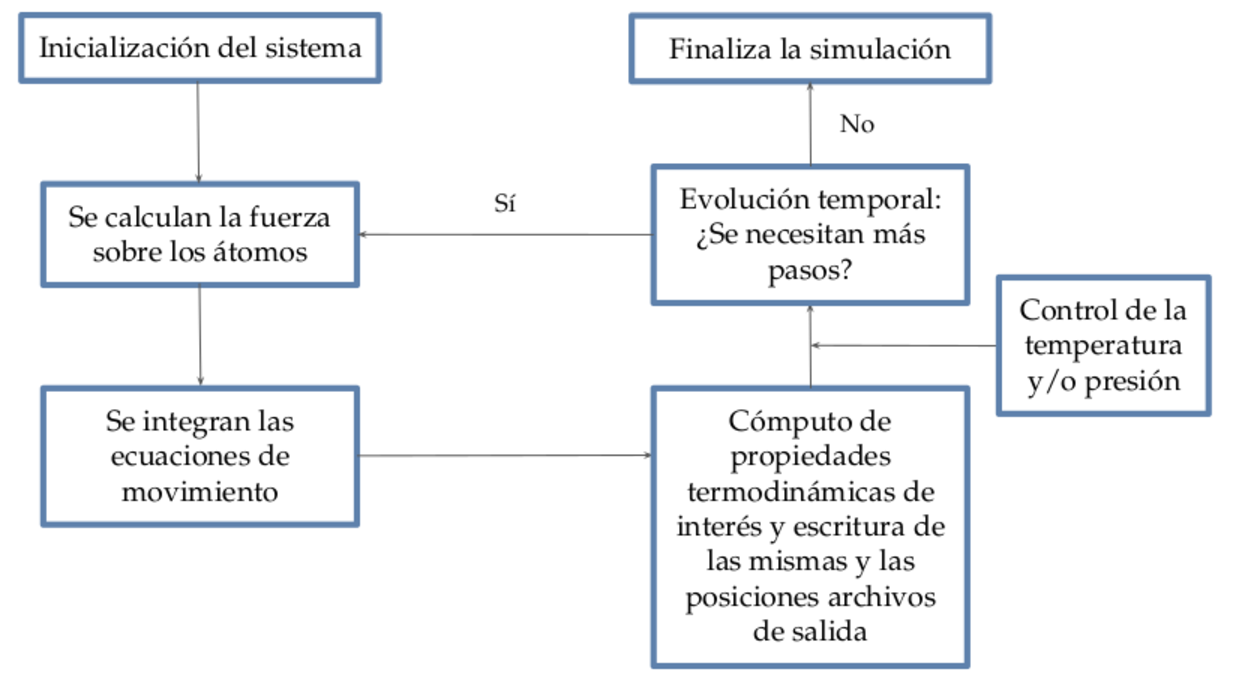
\includegraphics[width=\textwidth]{metodos/esquema_de_dinamica_molecular.pdf}
    \caption{Esquema de un diagrama de flujo de una dinámica molecular usual.}
    \label{fig:esquema_md}
\end{figure}

\subsection{Configuraciones iniciales}

Si bien las posiciones iniciales de algunos sistemas pueden reproducirse a partir
de los vectores de red de estructuras cristalinas, en otros casos de interés, en 
los cuales hay más de un elemento involucrado, las celdas unidad de mínimos 
locales son más complejas y han sido calculadas y optimizadas mediante la Teoría 
del funcional de la densidad electrónica (DFT, de sus siglas en inglés, density 
functional theory). Realizar estos cálculos suele ser una tarea
computacionalmente costosa y que requiere intervención de científicos 
especializados, para evitar este paso existe una base de datos ampliamente 
utilizada en el ámbito académico y en la industria, Materials Project 
~\cite{materials_project}, que recopila los datos que existen sobre estas 
estructuras cristalinas, realiza nuevos cálculos y está abierta a la comunidad 
para su uso y colaboración. Antes de que los datos se carguen en la página, los 
mismos son comparados con resultados experimentales para determinar si están 
dentro de un rango de validez definido. En esta tesis en particular, fueron 
utilizadas distintas estructuras cristalinas de esta base de datos como 
condiciones iniciales para las posiciones y los tamaños de las celdas de 
simulación.

Las velocidades de los átomos suelen ser generadas de manera aleatoria, a través
de un generador de números pseudo-aleatorio, tomando como argumento una semilla 
para la reproducibilidad de la simulación y una temperatura deseada para el
sistema. Estos números son generados con una distribución gaussiana, donde el 
centro se lo fija a cero para que no haya una velocidad en el centro de masa y 
el ancho está relacionado a la temperatura seleccionada.

\subsection{Condiciones de contorno}

Además de dar la configuración inicial de los átomos, es necesario especificar si
los mismos se encuentran dentro de una celda de simulación con un tamaño en
particular para cada una de las direcciones del sistema o si no interactúan fuera
del borde de la estructura que conforman los mismos. En el primero de los casos
se tienen condiciones periódicas de contorno (PBC, por sus siglas en inglés, 
\textit{periodic boundary conditions}), que busca reproducir un sistema infinito,
para que no existan efectos de borde, y consiste en considerar que los átomos se 
encuentran dentro de una celda unidad de una red infinita de celdas idénticas; en
donde si un átomo sale por un extremo de la celda, ingresa por el opuesto. Una
condición que debe cumplir esta celda es que su tamaño en cada una de las 
direcciones debe ser mayor al radio de corte de las interacciones entre los 
átomos. Por otro lado, el segundo de los casos es útil considerarlo cuando se 
tienen nanoestructuras en las cuales los átomos están ordenados de cierta forma 
que globalmente representan una forma definida y no pueden ser consideradas como
una red infinita.

\subsection{Potenciales interatómicos}

Los potenciales interatómicos empíricos o semi-empíricos que se utilizan en las
dinámicas moleculares relacionan la fuerza sobre un átomo con el entorno químico 
del mismo a través de una forma funcional conocida. Existe una gran 
variedad de estos potenciales y la elección de uno de ellos depende del sistema 
de estudio, ya que algunos potenciales representan de mejor manera gases y otros 
metales, por ejemplo. El potencial de Coulomb ~\cite{coulomb} considera las 
partículas como cargas puntuales que interactúan electrostáticamente. Los 
potenciales de Tersoff ~\cite{tersoff} o de Stillinger-Weber 
~\cite{stillinger-weber} fueron especialmente desarrollados para el modelado de 
materiales con enlaces covalentes fuertes, como es el caso del carbono o del 
silicio. El método del átomo embebido (EAM, de sus siglas en inglés) ~\cite{eam} 
y el EAM modificado (MEAM) ~\cite{meam} están diseñados para simular sistemas 
metálicos. Otros potenciales con enfoques más avanzados permiten simular
reacciones químicas en algunos sistemas, como es el caso de el COMB 
(\textit{charge-optimized many-body}) ~\cite{comb}, que incorpora una 
equilibración de las cargas en el modelo, o el del ReaxFF (\textit{reactive 
force fields}) ~\cite{reaxff}, que combina en un solo modelo distintas componentes
de las que fueron mencionadas.

Uno de los primeros potenciales utilizados en simulaciones computacionales fue 
el potencial interatómico de Lennard-Jones ~\cite{lennard-jones}, que reproduce 
el decaimiento de $r^{-6}$ a distancias largas y viene dado por la siguiente 
expresión
\begin{equation*}
V_{LJ} = 4\varepsilon \left[ \left( \frac{\sigma}{r} \right)^{12} - \left( \frac{\sigma}{r} \right)^{6} \right],
\end{equation*}
donde $r$ es la distancia entre dos átomos, $\varepsilon$ indica la profundidad 
del pozo del potencial que se encuentra en $r_m = 2^{1/6} \sigma$, $\sigma$ es el
radio del átomo. En la figura \ref{fig:lj} 
\begin{figure}
    \centering
    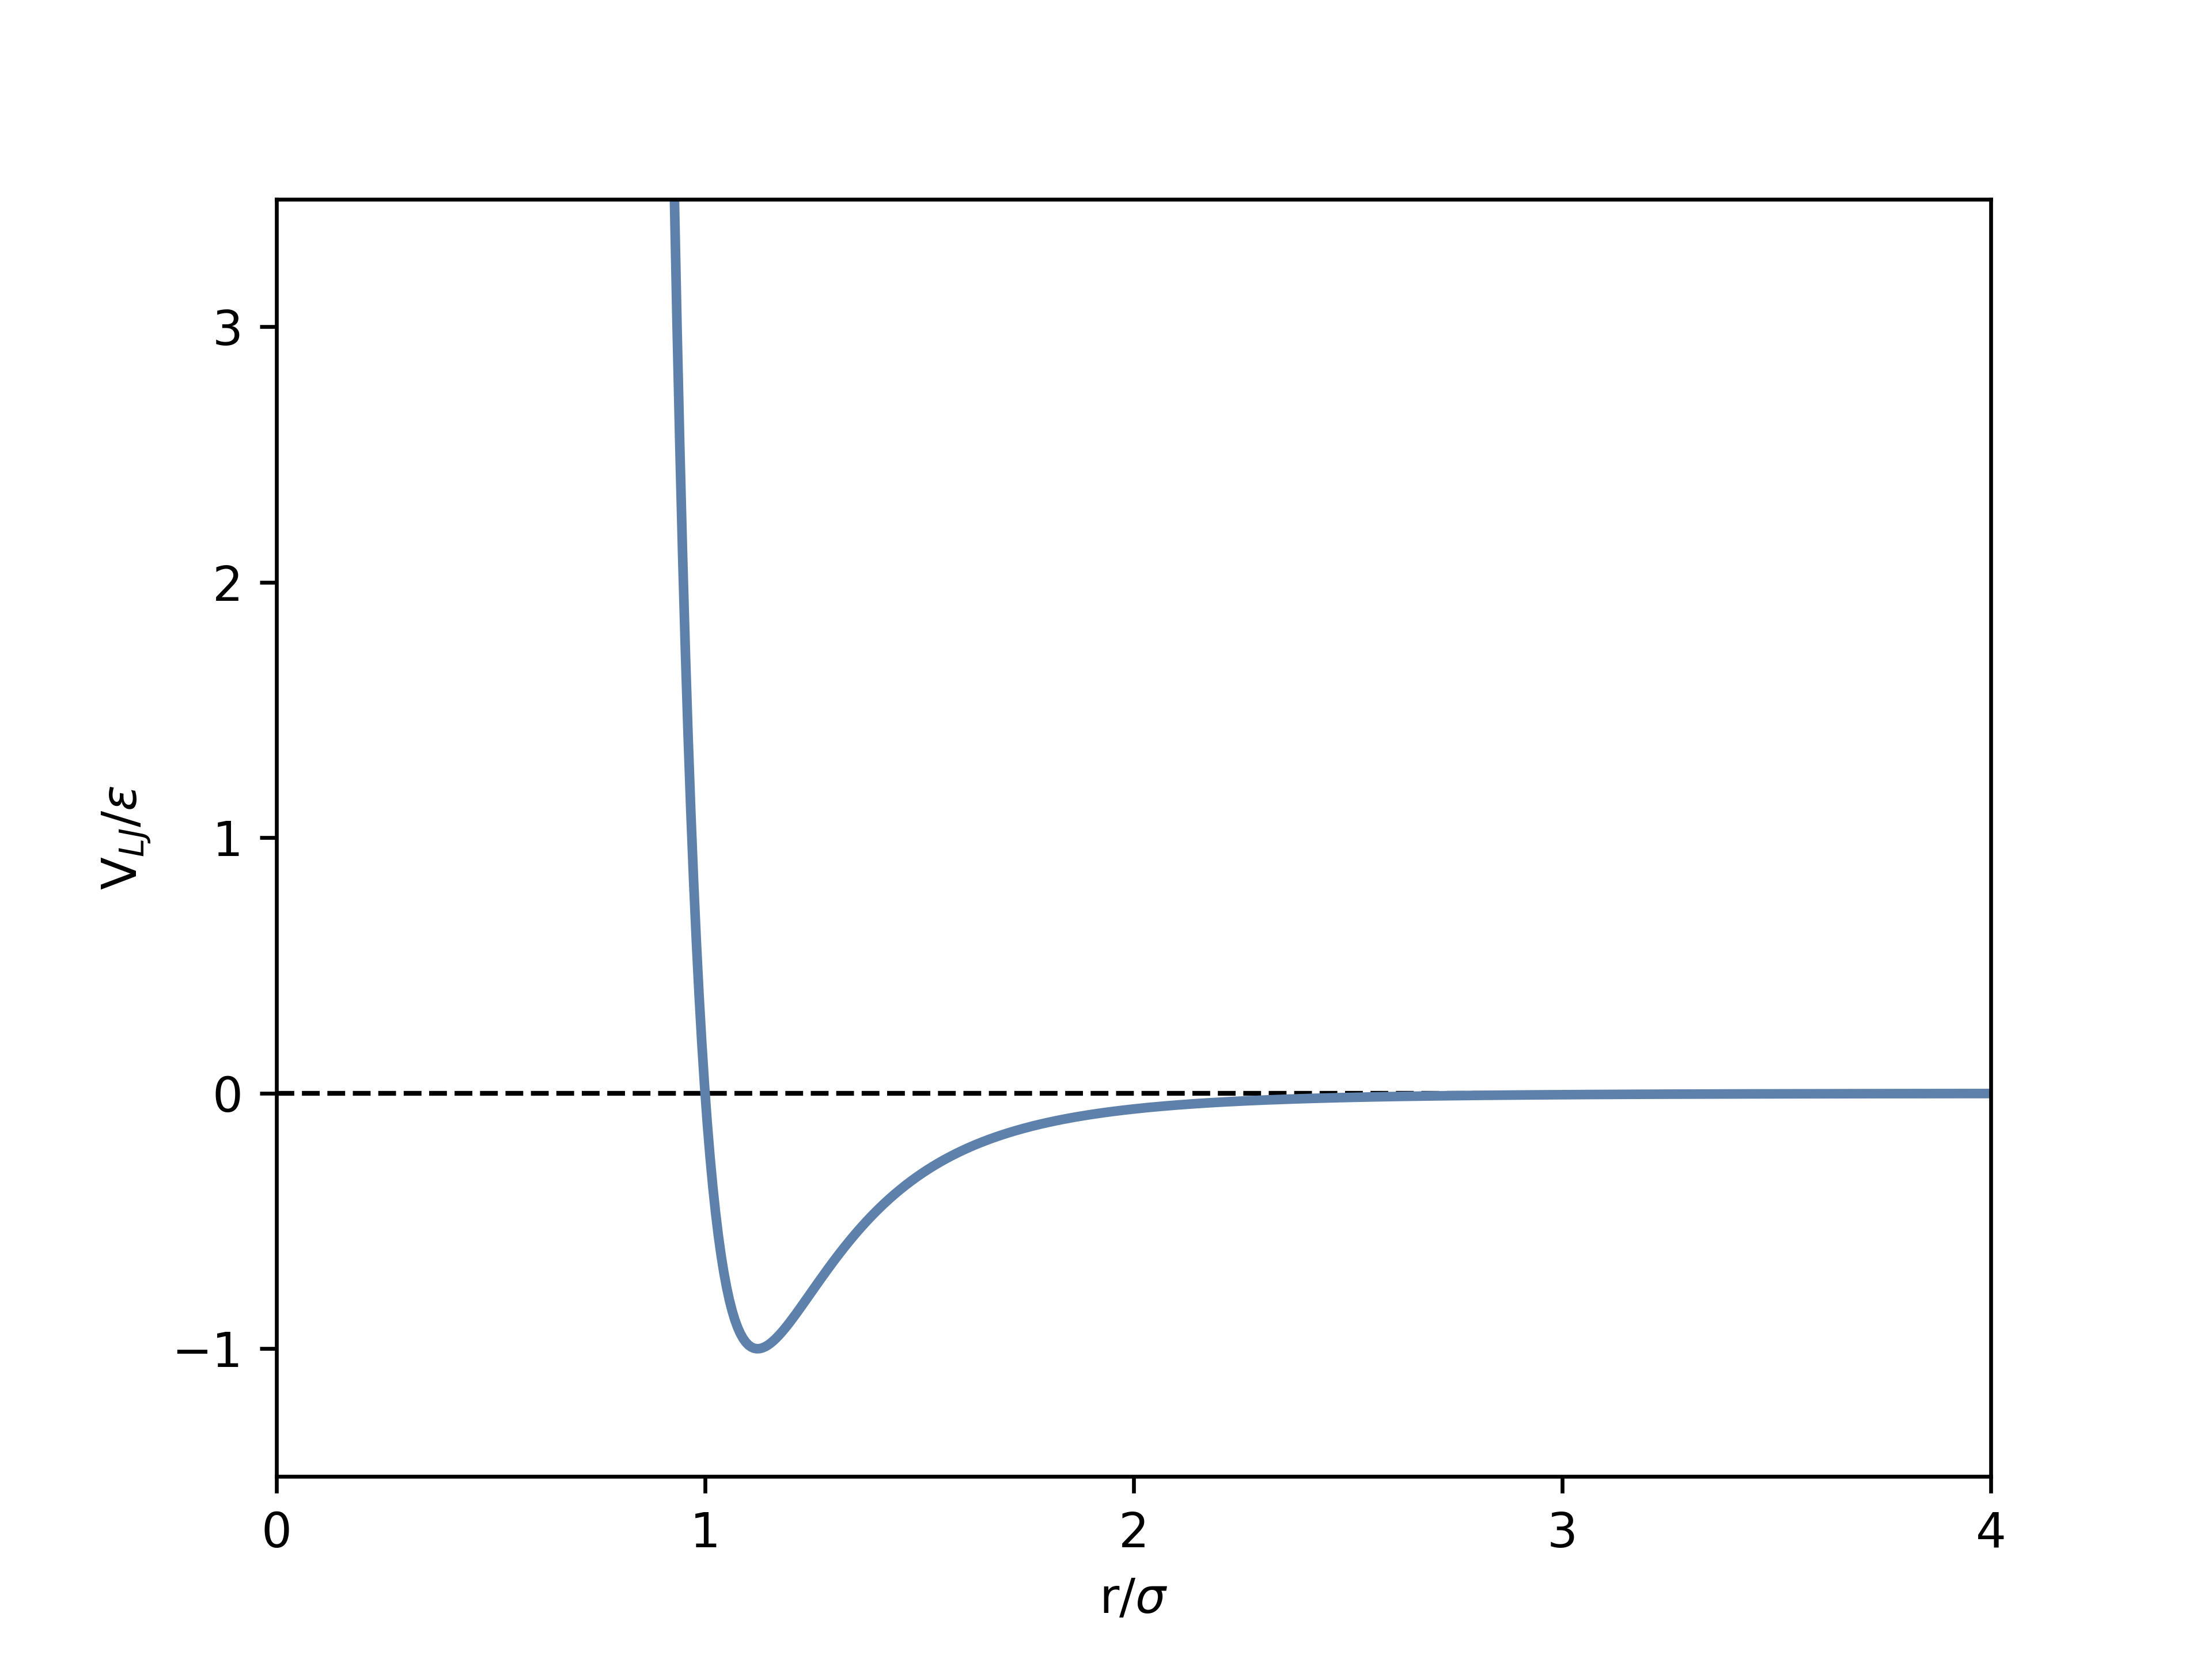
\includegraphics[width=0.7\textwidth]{metodos/lj.png}
    \caption{Gráfico de un potencial de Lennard-Jones.}
    \label{fig:lj}
\end{figure}
se muestra el comportamiento de este potencial, si la distancia entre dos
átomos es menor a $r_m$ entonces se repelen, si es mayor a dicha distancia, se 
atraen. Cuando la distancia entre dos átomos es infinita, los mismos no 
interactúan, en el caso práctico se define una distancia de corte, conocida como
el \textit{radio de corte}, $r_{cut}$, a partir de la cual se considera que el 
potencial es nulo. Para evitar discontinuidades en este punto se suelen utilizar 
distintas técnicas como el truncado y desplazado o se multiplica al potencial 
alrededor de dicho punto por una función suave, que hace que el potencial se 
iguale suavemente a cero.

Una vez que el potencial interatómico está bien definido, para calcular la fuerza
que actúa sobre el átomo $i$ es necesario computar la fuerza de a pares con todos
los átomos $j$ del sistema. Para esto es necesario calcular las distancias,
considerando la imagen mínima si las condiciones de contorno son PBC, y ver si
las mismas son mayores o menores a $r_{cut}$, si la distancia es mayor entonces
la contribución de esa interacción es igual a cero y si es menor se computa la 
fuerza a través del potencial de la siguiente manera
\begin{equation*}
f_x(r) = - \frac{\partial V(r)}{\partial x}
\end{equation*}
donde $x$ es la componente en alguna de las direcciones definidas para el sistema.

A continuación se presentan dos potenciales interatómicos del estado del arte que
fueron utilizados en esta tesis.

\subsubsection{ReaxFF}\label{s:reaxff}

El campo de fuerza reactivo, ReaxFF ~\cite{reaxff}, representa adecuadamente la
asociación y disociación de enlaces de átomos al considerar que la energía del 
sistema, $E_{system}$, se encuentra dividida en varias contribuciones de energías
parciales,
\begin{equation*}
E_{system} = E_{bond} + E_{over} + E_{under} + E_{val} + E_{pen} + E_{tors} + E_{conj} + E_{vdWaals} + E_{Coulomb}.
\end{equation*}

Una de las suposiciones fundamentales del ReaxFF es que el orden de enlace entre
un par de átomos puede obtenerse directamente de la distancia que los separa, 
esto es asegurado por el término $E_{bond}$.

$E_{over}$ y $E_{under}$ son términos agregados para imponer penalidades a los
átomos sobrecoordinados o subcoordinados, utilizando la teoría de la valencia 
del enlace.

$E_{val}$ considera la contribución a la energía por el ángulo de valencia, 
mientras que $E_{pen}$ penaliza sistemas para reproducir la estabilidad de 
sistemas con dos dobles enlaces que comparten un átomo en un ángulo de valencia.

Las contribuciones a la energía de los ángulos de torsión y de los efectos de 
conjugación están dados por $E_{tors}$ y $E_{conj}$, respectivamente.

Por último, las interacciones repulsivas a distancias interatómicas cortas y 
las atractivas a distancias largas son incluidas para todos los pares de átomos
mediante un término de van der Waals, $E_{vdWaals}$, utilizando un potencial de 
Morse, y uno de Coulomb, donde las cargas de los átomos se aproximan a través de 
un método de equilibración.

Los parámetros ajustables de los potenciales ReaxFF se obtienen a partir de 
cálculos de química cuántica sobre la disociación de enlaces, reacciones de 
moléculas pequeñas, calores de formación y geometrías de distintos compuestos.

\subsubsection{DFTB}

Un método alternativo para obtener las fuerzas en dinámica molecular es a través
de la utilización de un modelo híbrido entre los métodos \textit{ab-initio},
basados en DFT, y el uso de potenciales completamente empíricos, DFTB (de sus 
siglas en inglés, \textit{Density Functional based Tight Binding}), que tiene
la ventaja de ser más transferibles que estos últimos y requiere menos costo
computacional que los primeros.

El método de DFTB se basa en una expansión de segundo orden de la energía total 
de Kohn-Sham ~\cite{dft1, dft2} en la DFT con respecto a las fluctuaciones de la 
densidad de carga. El enfoque de orden cero es equivalente a un esquema estándar 
no auto-consistente (TB), mientras que en el segundo orden se puede derivar una 
expresión transparente, libre de parámetros y fácilmente calculable para los 
elementos matriciales hamiltonianos generalizados. Estos se modifican mediante 
una redistribución auto-consistente de las cargas de Mulliken (SCC).

La energía total de un sistema de $M$ electrones en el campo de $N$ núcleos en
las posiciones $\mathbf{R}$ puede escribirse a través de DFT como
\begin{equation*}
E = \sum_i^{occ} \langle \psi_i | - \frac{\Delta}{2} + V_{ext} + \frac{1}{2} \int' \frac{n(\mathbf{r}')}{|\mathbf{r} - \mathbf{r}'|} | \psi_i \rangle + E_{XC}(n(\mathbf{r})) + \frac{1}{2} \sum_{\alpha, \beta}^N \frac{Z_{\alpha}Z_{\beta}}{|\mathbf{R}_{\alpha} - \mathbf{R}_{\beta}|},
\end{equation*}
donde la primera suma es sobre los autoestados $\psi_i$ ocupados de Kohn-Sham,
$n(\mathbf{r})$ es la densidad electrónica, el segundo término es la contribución
de la correlación de intercambio (XC), y el último término considera la repulsión
de ion-ion. Si se utiliza una densidad de referencia $n_0$ más un término 
pequeño de fluctuación $\delta n$ y se expande $E_{XC}$ a la densidad de 
referencia:
\begin{equation}\label{eq:dft-fluc}
    \begin{aligned}
        E =& \sum_i^{occ} \langle \psi_i | \hat{H}_0 | \psi_i \rangle - \frac{1}{2} \int \int' \frac{n_0' n_0}{|\mathbf{r} - \mathbf{r}'|} + E_{XC}(n_0) - \int V_{XC}(n_0)n_0 + E_{ii} \\
        &+ \frac{1}{2} \int \int' \left(\frac{1}{|\mathbf{r} - \mathbf{r}'|} + \frac{\delta^2 E_{XC}}{\delta n \delta n'}\bigg\rvert_{n_0} \right)
    \end{aligned}
\end{equation}

\begin{enumerate}
    \item \textbf{Enforque de orden cero}

        El método de DFTB de orden cero calcula los elementos de la matriz 
        Hamiltoniana y de solapamiento a partir de una base orbital local con la
        ayuda de DFT-LDA (DFT-\textit{Local density approximation}) y algunas
        aproximaciones en las integrales. Puede verse como una aproximación de 
        una combinación lineal de los orbitales atómicos (LCAO, de sus siglas en 
        ingles, \textit{linear-combination-of-atomic-orbitals}). De esta forma se
        busca evitar las dificultades que surgen a la hora de parametrizar un 
        potencial empírico ~\cite{dftb1, dftb2}.

        En esta aproximación, las ecuaciones de Kohn-Sham son resultas de una
        forma no consistente, ignorando el último término de la ecuación 
        \ref{eq:dft-fluc} y expandiendo los orbitales de Kohn-Sham $\psi_i$ del 
        sistema en términos de las funciones de la base localizadas centradas en 
        el átomo,
        \begin{equation*}
        \psi_i = \sum_{\nu} C_{\nu i} \phi_{\nu}(\mathbf{r}-\mathbf{R}_k),
        \end{equation*}
        resolviendo las ecuaciones de Kohn-Sham para un potencial efectivo de una
        partícula $V_{eff}(\mathbf{r})$,
        \begin{equation}\label{eq:kohn-sham-mod}
            \hat{H}_0 \psi_i(\mathbf{r}) = \varepsilon_i \psi_i(\mathbf{r}), \quad \hat{H}_0 = \hat{T} + V_{eff}(\mathbf{r}),
        \end{equation}
        se tiene como resultado un conjunto de ecuaciones algebraicas,
        \begin{equation}\label{eq:alg-eq}
        \sum_{\nu} C_{\nu i} (H_{\mu \nu} - \varepsilon S_{\mu \nu}) = 0, \quad \forall \mu, i,
        \end{equation}
        donde
        \begin{equation*}
        H_{\mu \nu} = \langle \phi_{\mu}|\hat{H}_0|\phi_{\nu} \rangle, \quad S_{\mu \nu} = \langle\phi_{\mu}|\phi_{\nu}\rangle.
        \end{equation*}

        La energía total del sistema puede ser aproximada como una suma sobre la
        energía de la estructura de bandas y un potencial repulsivo de dos cuerpos
        de corto alcance,
        \begin{equation*}
            \begin{aligned}
                   E_{tot}(\{\mathbf{R}_k\}) &= E_{BS}(\{\mathbf{R}_k\}) + E_{rep}(\{|\mathbf{R}_k - \mathbf{R}_l|\}) \\
                    &= \sum_i n_i \varepsilon_i(\{\mathbf{R}_k\}) + \sum_k \sum_{<l} V_{rep}(|\mathbf{R}_l - \mathbf{R}_k|),
            \end{aligned}
        \end{equation*}
        donde $n_i$ es el número de ocupación del orbital $i$.
        
        Las funciones de onda pseudoatómicas pueden escribirse en términos de los
        orbitales tipo Slater y armónicos esféricos,
        \begin{equation*}
        \phi_{\nu}(\mathbf{r}) = \sum_{n,\alpha,l_{\nu},m_{\nu}} a_{n\alpha} r^{l_{\nu}+n} e^{-\alpha r} Y_{l_{\nu}m_{\nu}}\left(\frac{\mathbf{r}}{r}\right),
        \end{equation*}
        a la hora de realizar una solución auto-consistente a las ecuaciones
        modificadas de Kohn-Sham \ref{eq:kohn-sham-mod}. Estas soluciones son
        utilizadas como funciones de la base LCAO a la hora de tratar el sistema
        sólo considerando los orbitales de valencia.
        
        Como una aproximación, se escribe el potencial de un electrón de una 
        estructura con muchos átomos como una suma de contribuciones atómicas
        esféricas,
        \begin{equation*}
        V_{eff}(\mathbf{r}) = \sum_k V_0^k(|\mathbf{r} - \mathbf{R}_k|),
        \end{equation*}
        donde $V_0$ es el potencial de Kohn-Sham de un pseudo-átomo neutral.

        La matriz de solapamiento consiste solamente de dos elementos centrales
        y puede ser calculada de una forma sencilla
        \begin{equation*}
            H_{\mu\nu}^0 = 
            \begin{cases*}
                \varepsilon_{\mu}^{atomo\ libre} & si $\mu = \nu$ \\
                \langle \phi_{\mu}^{\alpha} | \hat{T} + V_0^{\alpha} + V_0^{\beta} | \phi_{\nu}^{\beta} \rangle & si $\alpha \neq \beta$ \\
                0 & para el resto de los casos,
            \end{cases*}
        \end{equation*}
        donde los índices $\alpha$ y $\beta$ indican el átomo sobre el cual la
        función de onda y el potencial están centrados, sólo dos elementos de la 
        matriz Hamiltoniana son tratados. Debido a que todos los elementos de la 
        matriz dependen sólo de las distancias interatómicas, sólo es necesario
        calcularlos una vez para cada par de tipo de átomo y guardar los valores
        definiendo un ancho de paso. Luego, los elementos para distancias 
        intermedias pueden ser interpolados entre los valores guardados.

        La repulsión a corto alcance $V_{rep}(R)$ puede ser determinada a partir
        de la diferencia en la energía total resultante de un cálculo 
        auto-consistente, $E_{LDA}^{sc}$, y $E_{BS}$ para distintos valores de 
        distancia $R$,
        \begin{equation*}
        V_{rep}(R) = E_{LDA}^{sc}(R) - E_{BS}(R).
        \end{equation*}

        Por último, las fuerzas interatómicas pueden ser derivadas de manera
        explícita para utilizarlas en dinámica molecular de la siguiente forma
        \begin{equation*}
        \mathbf{F}_{\alpha} = - \sum_i n_i \sum_{\mu} \sum_{\nu} C_{\mu i} C_{\nu i} \left(\frac{\partial H_{\mu \nu}^0}{\partial \mathbf{r}_{\alpha}} - \varepsilon \frac{\partial S_{\mu \nu}}{\partial \mathbf{r}_{\alpha}}\right) - \sum_{\beta \neq \alpha} \frac{\partial E_{rep}(|\mathbf{r_{\alpha} - \mathbf{r}_{\beta}|)}}{\partial \mathbf{r}_{\alpha}}.
        \end{equation*}

    \item \textbf{Enfoque de segundo orden}

        En una aproximación de segundo orden se agrega un término, además de
        el usual correspondiente a la \say{estructura de bandas} y el 
        potencial repulsivo de corto alcance, que considera la energía de
        interacción a largo alcance de Coulomb entre las fluctuaciones de la 
        carga a través una redistribución auto-consistente de las cargas de 
        Mulliken (SCC) ~\cite{dftb3}.

        Ahora sí se considera el último término de la ecuación \ref{eq:dft-fluc}
        al descomponer $\delta n(\mathbf{r})$ en contribuciones centradas en el
        átomo, entonces el término de segundo orden queda
        \begin{equation}\label{eq:q1}
        E_{2nd} = \frac{1}{2} \sum_{\alpha, \beta}^N \int \int' \Gamma(\mathbf{r}, \mathbf{r}', n_0) \delta n_{\alpha}(\mathbf{r}) \delta n_{\beta}(\mathbf{r}'),
        \end{equation}
        donde $\Gamma$ denota los coeficiente Hartree y XC. $\delta n_{\alpha}$
        puede ser extendida en una serie de funciones radiales y angulares,
        \begin{equation*}
            \begin{aligned}
                \delta n_{\alpha}(\mathbf{r}) &= \sum_{l,m} K_{ml} F_{ml}^{\alpha}(|\mathbf{r} - \mathbf{R}_{\alpha}|) Y_{lm} \left(\frac{\mathbf{r}-\mathbf{R}_{\alpha}}{|\mathbf{r}-\mathbf{R}_{\alpha}|}\right) \\
                &\approx \Delta q_{\alpha} F_{00}^{\alpha}(|\mathbf{r} - \mathbf{R}_{\alpha}|) Y_{00},
            \end{aligned}
        \end{equation*}
        donde $F_{ml}^{\alpha}$ denota la dependencia radial normalizada de la
        fluctuación de la densidad en el átomo $\alpha$ para el momento angular
        correspondiente. Esta expresión preserva la carga total del sistema.
        Si a la misma se la sustituye en la ecuación \ref{eq:q1},
        \begin{equation*}
        E_{2nd} = \frac{1}{2} \sum_{\alpha,\beta}^N \Delta q_{\alpha} \Delta q_{\beta} \gamma_{\alpha\beta},
        \end{equation*}
        donde
        \begin{equation*}
        \gamma_{\alpha\beta} = \int \int' \Gamma(\mathbf{r},\mathbf{r}',n_0)\frac{F_{00}^{\alpha}(|\mathbf{r} - \mathbf{R}_{\alpha}|)F_{00}^{\beta}(|\mathbf{r} - \mathbf{R}_{\beta}|)}{4 \pi}
        \end{equation*}
        se introduce como abreviatura. En el límite de distancias interatómicas
        grandes, $E_{2nd}$ puede ser vista como una interacción de Coulomb pura
        entre dos cargas puntuales $\Delta q_{\alpha}$ y $\Delta q_{\beta}$. Una
        aproximación simple y muy utilizada en métodos de química cuántica 
        semi-empíricos es aproximar el valor de $\gamma_{\alpha\alpha}$ por la 
        diferencia potencial de ionización atómica y la afinidad electrónica, que
        está relacionada al parámetro de Hubbard $U_{\alpha}$, 
        $\gamma_{\alpha\alpha} \approx U_{\alpha};$ luego, $\gamma_{\alpha\beta}$ 
        sólo depende de la distancia entre los átomos $\alpha$ y $\beta$ y los 
        parámetros $U_{\alpha}$ y $U_{\beta}$, que pueden ser calculados a partir 
        de la segunda derivada de la energía total de un solo átomo con respecto 
        al número de ocupación del último orbital atómico ocupado en LDA-DFT.

        Por último, en este enfoque de segundo orden, la ecuación 
        \ref{eq:dft-fluc} puede escribirse como
        \begin{equation*}
        E_2^{TB} = \sum_i^{occ} \langle \psi_i | \hat{H}_0 | \psi_i \rangle + \frac{1}{2} \sum_{\alpha, \beta}^N \gamma_{\alpha\beta} \Delta q_{\alpha} q_{\beta} + E_{rep}.
        \end{equation*}

        Para estimar las fluctuaciones de la carga se implementa el análisis de
        Mulliken
        \begin{equation*}
        q_{\alpha} = \frac{1}{2} \sum_i^{occ} n_i \sum_{\mu \in \alpha} \sum_{\nu}^N (C_{\mu i}^{*} C_{\nu i} S_{\mu nu} + C_{\nu i}^{*} C_{\mu i} S_{\nu mu})
        \end{equation*}
        y se obtiene un sistema de ecuaciones algebraicas como en la ecuación
        \ref{eq:alg-eq} pero donde el Hamiltoniano ahora considera una 
        corrección debido a la fluctuación de las cargas $H_{\mu \nu}^1$,
        \begin{equation*}
            \begin{aligned}
                H_{\mu \nu} &= \langle \phi_{\mu} | \hat{H}_0 | \phi_{\nu} \rangle + \frac{1}{2}\sum_{\xi}^N (\gamma_{\alpha\xi} + \gamma{\beta\xi}) \Delta q_{\xi} \\
                &= H_{\mu\nu}^0 + H_{\mu\nu}^1, \quad S_{\mu\nu} = \langle \phi_{\mu} | \phi_{\nu} \rangle, \quad \forall \mu \in \alpha, \quad \nu \in \beta.
            \end{aligned}
        \end{equation*}

        En este nuevo enfoque las fuerzas interatómicas para utilizar en 
        simulaciones de dinámica molecular vienen dadas por
        \begin{equation*}
        \mathbf{F}_{\alpha} = - \sum_i^{occ} n_i \sum_{\mu\nu} C_{\mu i} C_{\nu i} \left[\frac{\partial H_{\mu\nu}^0}{\partial \mathbf{r}_{\alpha}} - \left(\varepsilon_i - \frac{H_{\mu\nu}^1}{S_{\mu\nu}}\right) \frac{\partial S_{\mu\nu}}{\partial \mathbf{r}_{\alpha}} \right] - \Delta q_{\alpha} \sum_{\xi}^N \frac{\partial \gamma_{\alpha\xi}}{\partial \mathbf{r}_{\alpha}} \Delta q_{\xi} - \frac{\partial E_{rep}}{\partial \mathbf{r}_{\alpha}}.
        \end{equation*}
 
\end{enumerate}

\subsection{Integrador}

La funcionalidad que cumple un integrador en un código de dinámica molecular es
la de evolucionar las velocidades y las posiciones de los átomos una vez que 
ya se conocen las fuerzas que se aplican sobre cada uno de ellos. Un integrador
estándar, utilizado en esta tesis, fue el \textit{velocity Verlet}. El mismo 
conserva la energía total del sistema si no está siendo aplicado ningún termostato
o barostato que altere el ensamble. Para las posiciones se tiene una
actualización de las mismas, a partir del paso anterior, como un desarrollo de
Taylor
\begin{equation*}
r(t+dt) = r(t) + v(t) dt + \frac{f(t)}{2m} dt^2,
\end{equation*}
donde $dt$ es el paso temporal y $m$ la masa del átomo. Para las velocidades se
tiene
\begin{equation*}
v(t+dt) = v(t) + \frac{f(t+dt)+f(t)}{2m} dt,
\end{equation*}
es importante notar que para calcular la velocidad del paso temporal siguiente se
necesita tener computadas las fuerzas anteriores y posteriores, por lo cual
primero se calculan las posiciones y, a partir de ellas, las fuerzas.

Una característica a destacar de este integrador, además de conservar la energía
total del sistema, es que soporta una elección de pasos temporales más grandes
que integradores anteriores, esto hace que se simule el mismo tiempo real con 
menos pasos y por lo tanto menos cómputo de fuerzas, que es la parte 
computacionalmente más costosa del código.

\subsection{Cómputo de propiedades termodinámicas}

Una vez que ya se conocen las posiciones, velocidades y fuerzas de todos los 
átomos se tiene toda la información necesaria para computar distintas
cantidades de interés, el cómputo de cada una de ellas dependerá del ensamble en
el cual se están realizando las simulaciones.

Las energías que contribuyen a la energía total son dos, la potencial y la
cinética. La primera de ellas viene dada por distintas contribuciones de pares, 
ángulos, enlaces, etc, dependiendo de que tan complejo sea el campo de fuerzas 
utilizado. En el caso de que la interacción sea solo de a pares, la energía 
potencial puede calcularse de la siguiente forma
\begin{equation*}
E_{pot} = \sum_{i < j} u(r_{ij}),
\end{equation*}
donde $u(r_{ij})$ es la contribución proveniente de la interacción entre los 
átomos $i$ y $j$.

Por otro lado, la energía cinética traslacional puede calcularse a partir de las
velocidades de cada uno de los átomos como
\begin{equation*}
E_{cin} = \frac{1}{2} \sum_{i=1}^{N} m_i v_i^2, 
\end{equation*}
donde $m_i$ es la masa del átomo $i$ y $v_i^2$ el módulo de su velocidad. 

También suele ser de interés obtener el valor de la temperatura y de la presión
del sistema. La temperatura en un paso de la simulación puede calcularse 
utilizando que
\begin{equation}\label{eq:tempvel}
    k_B T = \sum_{i=1}^N \frac{m_i v_i^2}{N_f},
\end{equation}
donde $k_B$ es la constante del Boltzmann y $N_f$ los grados de libertad,
aproximados usualmente por $3N$ para sistemas lo suficientemente grandes. Por 
último, la presión puede calcularse como 
\begin{equation*}
P = \rho k_B T + \frac{1}{d V} \left\langle \sum_{i<j} \mathbf{f}(\mathbf{r}_{ij}) \cdot \mathbf{r}_{ij} \right\rangle,
\end{equation*}
donde $\rho$ es la densidad, $d$ la dimensión y $V$ el volumen del sistema. El
segundo término es conocido como el virial, donde $r_{ij}$ y $f(r_{ij})$ son las 
distancias y las fuerzas entre los átomos $i$ y $j$.

\subsection{Termostatos y barostatos}

Debido a que la dinámica molecular usual se realiza en el ensamble NVE y la 
mayoría de los experimentos con los cuales se pueden comparar resultados se 
realizan a temperatura y/o presión constante, es necesario introducir distintos
termostatos y barostatos que permitan controlar estos parámetros en las 
simulaciones realizadas. Para modelar el comportamiento directamente de estados
de equilibrio en estos ensambles, se puede modificar la dinámica molecular. Donde
estas modificaciones son meramente de conveniencia computacional y pueden producir 
desviaciones del movimiento newtoniano real, aunque extremadamente pequeñas.

Desde el punto de vista de la mecánica estadística a un sistema se le puede 
imponer una temperatura si se lo pone en contacto con un baño térmico lo 
suficientemente grande. En dicho caso la probabilidad de encontrar al sistema en
un estado de energía viene dada por la distribución de Maxwell-Boltzmann,
\begin{equation}\label{eq:mb}
P(v) = \left( \frac{\beta}{2\pi m} \right)^{3/2} exp(-\beta v^2 / (2m)),
\end{equation}
donde $\beta$ es la energía térmica $k_BT$. Esto quiere decir que la velocidad de
un átomo no se mantiene constante cuando está en contacto con un baño térmico, si 
no que la misma puede fluctuar y la fluctuación va a depender de dicha temperatura
de la siguiente forma
\begin{equation*}
\sigma_T^2 = \frac{2}{3 N} \langle T \rangle_{NVT}^2,
\end{equation*}
que proviene de calcular el segundo y el cuarto momento de la ecuación \ref{eq:mb}.

De manera análoga puede dejar de pensarse al volumen como constante y empezar a
pensar que el mismo es una variable cuando el sistema está acoplado a un pistón.

Distintos termostatos y barostatos fueron utilizados durante esta tesis, los mismos 
se introducen a continuación.

\subsubsection{MD a temperatura constante: Termostato de Langevin}

Si se considera la ecuación de Langevin \cite{schneider1978}
\begin{equation}\label{eq:langevin}
    m_i \dot{v_i} = F_i - m_i \gamma v_i + R_i(t),
\end{equation}
donde $F_i$ es la fuerza con la que interactúan los átomos entre sí, $\gamma$ la
constante de fricción y $R_i(t)$ es una variable estocástica con media cero 
y que cumple
\begin{equation*}
\left\langle R_i(t) R_j(t+t') \right\rangle = 2m_i \gamma_i k_B T \delta(t') \delta_{ij}.
\end{equation*}
Para aplicar este termostato, y simular a temperatura constante, en conjunto con 
el integrador \textit{velocity Verlet} se tienen que considerar tres parametros
\cite{kroger2005} a la hora de actualizar las velocidades y las posiciones como
\begin{equation*}
a = \frac{2 - \xi dt}{2 + \xi dt},
\end{equation*}
\begin{equation*}
b= \sqrt{k_B T_0 \xi \frac{dt}{2}},
\end{equation*}
\begin{equation*}
c= \frac{2 dt}{2 + \xi dt}
\end{equation*}
donde $\xi$ es el factor de fricción, es decir, con qué intensidad interacciona 
el sistema con el baño térmico. Se tiene entonces una actualización se la siguiente
manera
\begin{equation*}
v(t+dt) = a v(t) + b \eta + \frac{f(t+dt)+f(t)}{2m} dt,
\end{equation*}
\begin{equation*}
r(t+dt) = r(t) + c v(t) dt
\end{equation*}
donde $\eta$ es una distribución gaussiana de números aleatorios con media 0 y
varianza 1. 

\subsubsection{MD a temperatura y/o presión constante: Termostato y Barostato 
de Berendsen}

El termostato de Berendsen \cite{berendsen1984} puede derivarse si se considera 
la ecuación \ref{eq:langevin} sin el término estocástico y se hace una elección
en particular de la constante de fricción. Dicha ecuación de movimiento modificada
representa un escaleo de velocidades, 
\begin{equation*}
v(t) = \lambda v(t),
\end{equation*}
por paso temporal, donde
\begin{equation*}
\lambda = \sqrt{1 + \frac{dt}{\tau_T} \left( \frac{T_0}{T} - 1 \right)}
\end{equation*}
produce un cambio de temperatura igual a
\begin{equation*}
\frac{dT}{dt} = \frac{1}{\tau_T} (T_0 - T)
\end{equation*}
donde $T_0$ es la temperatura de referencia y  $\tau_T$ es la constante de
acoplamiento con el baño térmico y tiene las mismas unidades que el paso temporal.

Para considerar un acoplamiento con un baño de presión contante, Berendsen 
\cite{berendsen1984} agrega un término extra a las ecuaciones de movimiento que
consideran el cambio de presión
\begin{equation*}
\frac{dP}{dt} = \frac{P_0 - P}{\tau_P},
\end{equation*}
donde $P_0$ es la presión de referencia, $P$ la instantánea y $\tau_P$ la 
constante de acoplamiento. Este comportamiento puede producirse si se realiza un
cambio en el virial, escaleando las distancias entre las partículas. Si el 
volumen ahora cambia como 
\begin{equation*}
\frac{dV}{dt} = 3 \alpha V,
\end{equation*}
y se usa que
\begin{equation*}
\frac{dP}{dt} = - \frac{1}{\beta V} \frac{dV}{dt} = -\frac{3\alpha}{\beta},
\end{equation*}
donde $\beta$ es la compresibilidad isotérmica y $\alpha = - \beta (P_0 - P) / (3 \tau_P)$.
Por lo cual las posiciones de los átomos dentro de la caja de simulación en cada
dirección pueden escalearse como
\begin{equation*}
x = \mu x,
\end{equation*}
donde
\begin{equation*}
\mu = \sqrt[3]{1 - \frac{dt}{\tau_P} (P_0 - P)}.
\end{equation*}

\subsubsection{MD a temperatura constante: Termostato de Nosé-Hoover}

Debido a que la temperatura es proporcional al promedio de las velocidades al 
cuadrado, como puede verse en la ecuación \ref{eq:tempvel}, es posible variar
la temperatura al ajustar la razón a la cual el tiempo progresa 
~\cite{nose1984a}. Por lo cual puede introducirse una nueva variable dinámica
$s$ en el Lagrangiano que reescalee la unidad de tiempo, y se añaden términos 
adicionales para obtener el comportamiento deseado ~\cite{rapaport2004}. Lo que 
que provoca que haya dos variables temporales distintas: el tiempo real, o físico, 
$t'$, y un tiempo escalado, o virtual, $t$; que están relacionados a través de 
sus diferenciales,
\begin{equation*}
dt = s(t') dt'.
\end{equation*}
El Lagrangiano de este sistema extendido se escribe como
\begin{equation*}
\mathcal{L} = \frac{1}{2} m s^2 \sum_i \dot{\mathbf{r}}_i^2 - \sum_{i<j} u(\mathbf{r}_{ij}) + \frac{1}{2} M_s \dot{s}^2 - n_f T \log s,
\end{equation*}
donde $T$ es la temperatura deseada, $n_f = 3N_m + 1$ el número de grados de 
libertad, $M_s$ es una masa que se necesita para construir la ecuación de 
movimiento de la nueva \say{coordenada} $s$ y el punto representa la derivada
con respecto al tiempo virtual. Las ecuaciones de movimiento de Lagrange pueden 
obtenerse de la forma usual y son
\begin{equation*}
\ddot{\mathbf{r}}_i = \frac{1}{m s^2} \mathbf{f}_i - \frac{2 \dot{s}}{s} \dot{\mathbf{r}}_i
\end{equation*}
\begin{equation*}
M_s \ddot{s} = m s \sum_i \dot{\mathbf{r}}_i^2 - \frac{n_f T}{s}
\end{equation*}

Ya que la relación entre t y t' depende de toda la historia del sistema, es decir,
\begin{equation*}
t = \int s(t') dt'
\end{equation*}
es más conveniente si las ecuaciones se transforman a las unidades del tiempo
físico ~\cite{nose1984b, hoover1985}, ahora el punto pasa a representar la 
derivada con respecto al tiempo real, y las ecuaciones de movimiento pueden 
reescribirse como
\begin{equation*}
\ddot{\mathbf{r}}_i = \frac{1}{m} \mathbf{f}_i - \frac{\dot{s}}{s} \dot{\mathbf{r}}_i
\end{equation*}
\begin{equation*}
\ddot{s} = \frac{\dot{s}^2}{s} + \frac{G_1 s}{M_s} 
\end{equation*}
donde $G_1 = m \sum_i \dot{\mathbf{r}}_i^2 - n_f T$. La primera de estas 
ecuaciones de movimiento se asemeja a la ecuación newtoniana convencional con un 
término adicional similar al de la fricción, aunque no se trata de una fricción 
verdadera ya que el coeficiente puede ser de cualquier signo. La segunda ecuación 
define el mecanismo de retroalimentación por el que $s$ varía para regular la 
temperatura.

Si se integra la función partición microcanónica del sistema extendido sobre la
variable $s$ se obtiene la función de partición canónica, lo cual demuestra que
los promedios de equilibrio del sistema físico son los del ensamble canónico a
temperatura $T$ ~\cite{nose1984a}. Sin embargo, la temperatura en sí no es 
constante, pero la retroalimentación negativa que actúa a través de $s$ garantiza
que las fluctuaciones sean limitadas y el valor medio sea igual a $T$.

El Hamiltoniano del sistema extendido
\begin{equation*}
\mathcal{H} = \frac{1}{2} m \sum_i \dot{\mathbf{r}}_i^2 + \sum_{i<j} u(\mathbf{r}_{ij}) + \frac{1}{2} M_s \left(\frac{\dot{s}}{s}\right)^2 + n_f T \log s
\end{equation*}
se conserva debido a que no hay fuerzas externas que dependan del tiempo, lo cual 
proporciona una comprobación útil de la precisión de la solución numérica. El 
Hamiltoniano no tiene significado físico, sus dos primeros términos representan 
la energía del sistema físico, pero su suma es libre de fluctuar.

La $M_s$ no tiene ningún significado físico en particular, simplemente es una 
parte de la técnica computacional de cálculo y su valor debe determinarse 
empíricamente, que, en principio, no afecta a los resultados de equilibrio final, 
pero sí influye en su precisión y confiabilidad. Para variaciones pequeñas de $s$, 
el período característico de las fluctuaciones es ~\cite{nose1984a}
\begin{equation*}
\tau_s = 2 \pi \sqrt{\frac{M_s \langle s \rangle^2}{2 n_f T}}
\end{equation*}
y la simulación debe extenderse a lo largo de muchos de estos períodos para evitar 
que estas fluctuaciones influyan negativamente en los resultados.

De una manera similar a la realizada en el algoritmo de Nosé-Hoover para el 
control de la temperatura, el algoritmo de \textbf{Parrinello-Rahman} permite
obtener una representación correcta del ensamble isotérmico-isobárico al 
realizar un \textbf{control de la presión}, donde se permite una evolución 
temporal del volumen de la caja ~\cite{parrinello-rahman}.


\subsection{Observables}\label{s:observables}

Existen distintos observables que pueden calcularse a partir de las posiciones o
de las velocidades a lo largo de una trayectoria proveniente de una dinámica 
molecular, algunos de ellos dan información de carácter estructural, como puede 
ser la distribución radial de a pares, y otros de dinámico, como el 
desplazamiento cuadrático medio que puede ser utilizado para estimar 
coeficientes de difusión.

\subsubsection{Distribución radial de a pares}

La función de distribución radial de a pares (RDF, de sus siglas en inglés
\textit{radial distribution function}), usualmente referida como $g(r)$, permite 
caracterizar la estructura local de un fluido describiendo la probabilidad de 
encontrar un átomo en una cáscara a una distancia $r$ de un átomo de referencia,
\begin{equation*}
g(r) = \frac{V}{N^2} \left\langle \sum_{i=1, i\neq j}^N \delta(\vec{r} - \vec{r}_{ij}) \right\rangle,
\end{equation*}
donde $\langle \cdot \rangle$ indica el promedio temporal, $V$ el volumen, $N$ el
número de partículas y $\vec{r}_{ij}$ la distancia entra la partícula $i$ y la $j$.
Esta cantidad puede calcularse como la razón entre la densidad media $\rho$ a
una distancia $r$ del átomo de referencia y la densidad a esa misma distancia de 
un gas ideal.

Una característica importante de la RDF es que si sus picos están bien definidos
entonces la estructura se corresponde con un sólido, si sus picos están ensanchados
con respecto a estos y, a medida que la distancia aumenta, la $g(r)$ empieza a 
oscilar alrededor de la unidad, entonces se corresponde con un liquido.

\subsubsection{Número de coordinación}

El número de coordinación (CN, de sus siglás en inglés, \textit{coordination 
number}), también llamado ligancia, de un átomo dado en un sistema químico, se 
define como el número de átomos, moléculas o iones unidos a él. Para definirlo 
pueden tomarse dos alternativas, la primera de ellas contando el número de 
vecinos que rodean a un determinado tipo de átomo en promedio hasta un cierto
radio de corte $r_e$, definido por el mínimo en la RDF después de su primer 
pico; la segunda de ellas a partir de la integral de la RDF,
\begin{equation*}
\int_0^{r_e} g(r) dV.
\end{equation*}
De manera análoga pueden definirse el número de coordinación para segundos 
vecinos y así sucesivamente.

\subsubsection{Difusión}

Si una partícula permanece en un sitio por un periodo de tiempo lo suficientemente 
largo, comparado al tiempo que demora en dar un salto hacia otro sitio, entonces 
pierde memoria de donde vino y el próximo salto se dará hacia una dirección 
aleatoria, se dice entonces que el movimiento de la partícula es estocástico y 
que sigue una caminata aleatoria. Si esto se cumple, entonces, el desplazamiento 
cuadrático medio es proporcional al tiempo, donde la constante de proporcionalidad 
es el coeficiente de difusión de traza
\begin{equation}
    D^{*} = \frac{\langle \Delta r^2 \rangle}{2d\cdot t},
\end{equation}
donde $d$ es la dimensión del problema, $t$ el tiempo y 
$\langle \Delta r^2 \rangle$ el desplazamiento cuadrático medio, que en un sistema 
de $N$ partículas puede calcularse de la siguiente manera
\begin{equation*}
\langle \Delta r^2 \rangle = \frac{1}{N} \sum_{i=1}^{N} \langle |\vec{r_i}(t) - \vec{r_i}(t_0)|^2 \rangle.
\end{equation*}

Si se conoce el coeficiente de difusión de traza, entonces el coeficiente de 
difusión químico puede obtenerse de la siguiente relación ~\cite{gomer1990}
\begin{equation}
    D = \left( \frac{\partial (\mu / k_BT)}{\partial ln \theta} \right)_T D^{*},
\end{equation}
donde $\mu$ es el potencial químico y $\theta$ es la concentración.

Usualmente, el tiempo que demora un átomo en dar un salto en una dinámica 
molecular a temperatura ambiente es muy largo, lo que impide tener una buena 
estadística en un tiempo de simulación razonable, por lo que es usual calcular 
el desplazamiento cuadrático medio a distintas temperaturas altas y extrapolar
el valor que se obtendría a temperatura ambiente mediante una ecuación de tipo 
Arrhenius, en la cual el coeficiente de difusión puede separarse en un 
prefactor $D_0$ y un término tipo Boltzmann,
\begin{equation*}
D = D_0 e^{-E / k_BT},
\end{equation*}
donde $E$ es la energía de activación del proceso. 


\section{Software}

En la actualidad existe una gran cantidad de códigos que permiten realizar 
simulaciones de dinámica molecular de manera eficiente aprovechando la estructura
paralela de los procesadores. En esta tesis se utilizó principalmente \path{LAMMPS} 
(\textit{Large-scale Atomic/Molecular Massively Parallel Simulator}, sus siglas
en inglés) ~\cite{lammps1, lammps2}, un código centrado en el modelado de 
materiales que permite simular con distintos campos de fuerzas, ensambles y 
condiciones de contorno. También se realizaron simulaciones con versiones 
modificadas de \path{GEMS} ~\cite{gems}, código del Dr. Sergio Alexis Paz 
(FCQ-UNC), que permiten utilizar a \path{DFTB+} ~\cite{dftb+} como una librería
y realizar distintos métodos de aceleración de simulaciones que no se encuentran
en los programas usuales como \path{LAMMPS}.

Para la visualización de las trayectorias y la obtención de imágenes de 
estructuras representativas se utilizó \path{VMD} (\textit{Visual Molecular 
Dynamics}) ~\cite{vmd}. Para el post-procesamiento de datos de las simulaciones
se escribieron distintos programas en Python ~\cite{exma, sierras}.



\chapter[Caracterización de estructuras amorfas en ánodos de Silicio]{
    Caracterización de estructuras amorfas en ánodos de Silicio}
\thispagestyle{empty}

\vspace{50pt}

\begin{adjustwidth}{50pt}{50pt}
    En este capítulo se caracterizan estructuralmente las aleaciones amorfas de
    Li$_x$Si a distintas concentraciones, mediante simulaciones computacionales,
    utilizando un campo de fuerzas reactivo y una exploración acelerada de mínimos
    locales propuesta aquí para encontrar estructuras cercanas al equilibrio. Se
    analiza la distribución radial de a pares, los números de coordinación de los
    primeros y segundos vecinos más cercanos y el ordenamiento a corto alcance.
    Además, la estructura compleja del segundo pico de la $g(r)$ de Si-Li es 
    dilucidada a partir de un análisis de interconexión de clusters.
\end{adjustwidth}

\clearpage
\newpage
\thispagestyle{empty}
\mbox{}
\newpage

\chapter[Caracterización de estructuras amorfas en ánodos de Silicio]{
    Caracterización de estructuras amorfas en ánodos de Silicio}
\thispagestyle{empty}

\vspace{50pt}

\begin{adjustwidth}{50pt}{50pt}
    En este capítulo se caracterizan estructuralmente las aleaciones amorfas de
    Li$_x$Si a distintas concentraciones, mediante simulaciones computacionales,
    utilizando un campo de fuerzas reactivo y una exploración acelerada de mínimos
    locales, propuesta aquí para encontrar estructuras cercanas al equilibrio. Se
    analiza la distribución radial de a pares, los números de coordinación de los
    primeros y segundos vecinos más cercanos y el ordenamiento a corto alcance.
    Además, la estructura compleja del segundo pico de la $g(r)$ de Si-Li es 
    dilucidada a partir de un análisis de interconexión de clusters.
\end{adjustwidth}

\clearpage
\newpage
\thispagestyle{empty}
\mbox{}
\newpage


La información experimental que puede obtenerse de la estructuras de las 
distintas fases amorfas que se forman durante el ciclado de los electrodos de 
silicio es bastante limitada. Estas estructuras son 
inestables y amorfas, lo cual dificulta su caracterización mediante técnicas
experimentales tradicionales. Por ejemplo, la difracción de rayos x permitió
caracterizar la fase cristalina Li$_{15}$Si$_4$ que está presente en el electrodo
cuando este se encuentra completamente cargado ~\cite{obrovac2004}, pero esta 
técnica tiene ciertas limitaciones a la hora de estudiar estructuras amorfas 
que se encuentran en los procesos de carga y descarga. Por otro lado, el análisis
de la función distribución de a pares de Si \textit{ex-situ} de datos de rayos x
hizo posible investigar el orden a corto alcance de las estructuras amorfas de
Li$_x$Si ~\cite{key2011} y proponer una explicación al mecanismo de litiación.
Sin embargo, como los elementos livianos como el Li tienen baja sensibilidad a 
los rayos x, las conclusiones están restringidas a la formación de pequeños 
clusters de Si o de átomos de Si aislados durante la litación, lo cual limita la 
descripción de la estructura a una escala mayor.

Dentro de este contexto, las simulaciones computacionales se posicionan como una
herramienta poderosa para acceder al comportamiento microscópico de las 
estructuras de Li$_x$Si y los cambios que sufren durante la litiación. Actualmente
no existe un único modelo computacional robusto que permita estudiar todos los
diferentes procesos presentes en los electrodos de silicio, por lo que se han 
llevado a cabo distintos esfuerzos en los últimos años para estudiar este sistema,
donde el mayor obstáculo está relacionado con la naturaleza intrínseca de 
multi-escala del silicio. A pesar de su gran precisión, los estudios de DFT se
encuentran drásticamente limitados en el número de átomos que se pueden utilizar
para modelar las estructuras complejas de las fases litiadas. Una solución a este
problema es utilizar potenciales interatómicos semi-empíricos, para los cuales 
se necesita una parametrización que se robusta y transferible. En este 
capítulo se utiliza un potencial reactivo, introducido en 
la sección \ref{s:reaxff}, para sistemas de Li-Si previamente realizada por Fan 
\textit{et al.} ~\cite{fan2013}, en la cual optimizaron el campo de fuerzas usando
cálculos de DFT, considerando datos de las energías, distintas geometrías y cargas
de las fases cristalinas de Li, Si y aleaciones de Li-Si. En su trabajo lo 
utilizaron en simulaciones de MD para caracterizar las propiedades mecánicas de
las estructuras amorfas de Li$_x$Si, incluyendo litiación de capa fina, compresión
biaxial, tensión y compresión uniaxial y la tensión que puede soportar el sistema 
antes de deformarse.


\section{Campo de fuerzas}

El campo de fuerzas de Fan \textit{et al.} ha sido ampliamente utilizado en 
simulaciones de MD para estudiar el proceso de litiación de distintas estructuras
de silicio, desde estructuras periódicas a nanoestructuras. Previo a la 
realización del trabajo de este capítulo, se consultó la bibliografía para 
verificar esto y asegurarnos de la transferibilidad del potencial. 

Además de los resultados reportados por Fan \textit{et al.} ~\cite{fan2013}, 
la estructura, el estrés y la difusividad fue estudiada durante la litiación de 
silicio amorfo (a-Si) y silicio cristalino (c-Si) en diferentes orientaciones 
cristalográficas ~\cite{chen2020, kim2015}. Ding \textit{et al.} ~\cite{ding2017} 
reportó la variación de la velocidad de migración en la frontera de fases y la 
difusividad de Li en función del estrés externo aplicado, exponiendo que la 
tensión acelera la velocidad de litiación, mientras que la compresión la retarda. Kim 
\textit{et al.} ~\cite{kim2014} realizó simulaciones de MD para caracterizar la 
evolución estructural de la frontera de fases entre c-Si, con diferentes planos 
de orientación, con una fase amorfa de litiación máxima. Posteriormente, Fan 
\textit{et al.} ~\cite{fan2018} estudió nanoestructuras, computando la respuesta
mecánica de nanopilares de c-Si en la orientación (111) durante la litiación.
Un trabajo similar, pero para la orientación (100), fue realizado por Cao 
\textit{et al.} ~\cite{cao2019}. Tang \textit{et al.} ~\cite{tang2019} investigó
la evolución y la permanencia de la porosidad de nanocapas de Si durante los 
procesos de litiación y delitiación. Ostadhossein \textit{et al.} 
~\cite{ostadhossein2015} caracterizó la litiación de nanohilos de c-Si y mostró
que este potencial ReaxFF reproduce en forma precisa las barreras de energía de la
migración de Li obtenidas por DFT, tanto en c-Si como en a-Si.

La aplicación de este potencial no estuvo sólo limitada a simulaciones de MD, sino que fue empleado en otros
métodos de simulación, por ejemplo, simulaciones de Monte Carlo en el ensamble
gran canónico, que fueron realizadas para estudiar un ciclo de litiación y delitiación
de un electrodo de a-Si ~\cite{basu2019}. Trochet y Mousseau ~\cite{trochet2017}
caracterizaron el paisaje energético a concentraciones relativamente bajas de 
impurezas de Li en c-Si, usando una técnica de activación-relajación cinética. 
Kim \textit{et al.} ~\cite{kim2017} desarrollaron un algoritmo para investigar la 
respuesta a la delitiación de una capa delgada de silicio recubierta de óxido de 
aluminio. El ReaxFF también fue combinado con otros campos de fuerza, como los
potenciales de Tersoff y Lennard-Jones, para simular la litiación de 
nanopartículas de Si recubiertas con carbono, que permitieron observar una 
correlación entre el crecimiento del estrés y la densidad de carga 
~\cite{zheng2019,zheng2020}. Propiedades mecánicas de interfase Si/SiO$_2$ litiada
fueron reportadas por Verners y Simone ~\cite{verners2019}. 

No es posible llevar a cabo un estudio sobre las propiedades electrónicas con el 
uso del ReaxFF, ya que esta es una de sus limitaciones.  Sin embargo, de la discusión 
previa, puede observarse que ha sido capaz de predecir un número importante de
propiedades del sistema Li-Si.


\section{Configuraciones iniciales}

\subsection{Estructuras cristalinas}

En este capítulo se estudian las propiedades de las estructuras amorfas Li$_x$Si
para distintos valores de $x$ en un rango que va de 0.21 a 4.2. Para algunas de
estas concentraciones se encuentran estructuras cristalinas, las cuales 
fueron extraídas del Materials Project ~\cite{materials_project} 
(mp-1314, mp-672287, mp-569849, mp-29720) y sus posiciones utilizadas para definir
los estados iniciales. Las celdas primitivas de las estructuras cristalinas se
muestran en la figura \ref{fig:cristalinas}, donde están en orden creciente de 
concentración de Li. Las mismas son Si, LiSi, Li$_{12}$Si$_7$, Li$_7$Si$_3$, 
Li$_{13}$Si$_4$, Li$_{15}$Si$_4$, Li$_{21}$Si$_5$ y Li. En la estructura de LiSi
se tiene una remanencia del diamante de Si en los enlaces, en la Li$_{12}$Si$_7$ 
hay dos tipos de clusters de átomos de Si, pentágonos y estrellas, en la
Li$_7$Si$_3$ los átomos de Si se encuentran en mancuernas, en la Li$_{13}$Si$_4$ 
se tienen las mismas mancuernas junto a algunos átomos aislados y, por último, 
todos los átomos de Si se encuentran aislados tanto en la Li$_{15}$Si$_{4}$ como
en la Li$_{21}$Si$_5$. Estas estructuras cristalinas fueron observadas a 
temperaturas altas ~\cite{wen1981}, pero no se encuentran en el funcionamiento de
una batería ~\cite{obrovac2004}. Sin embargo, sus posiciones pueden tomarse como 
iniciales para simular estructuras amorfas a las concentraciones correspondientes.
\begin{figure}[t]
    \centering
    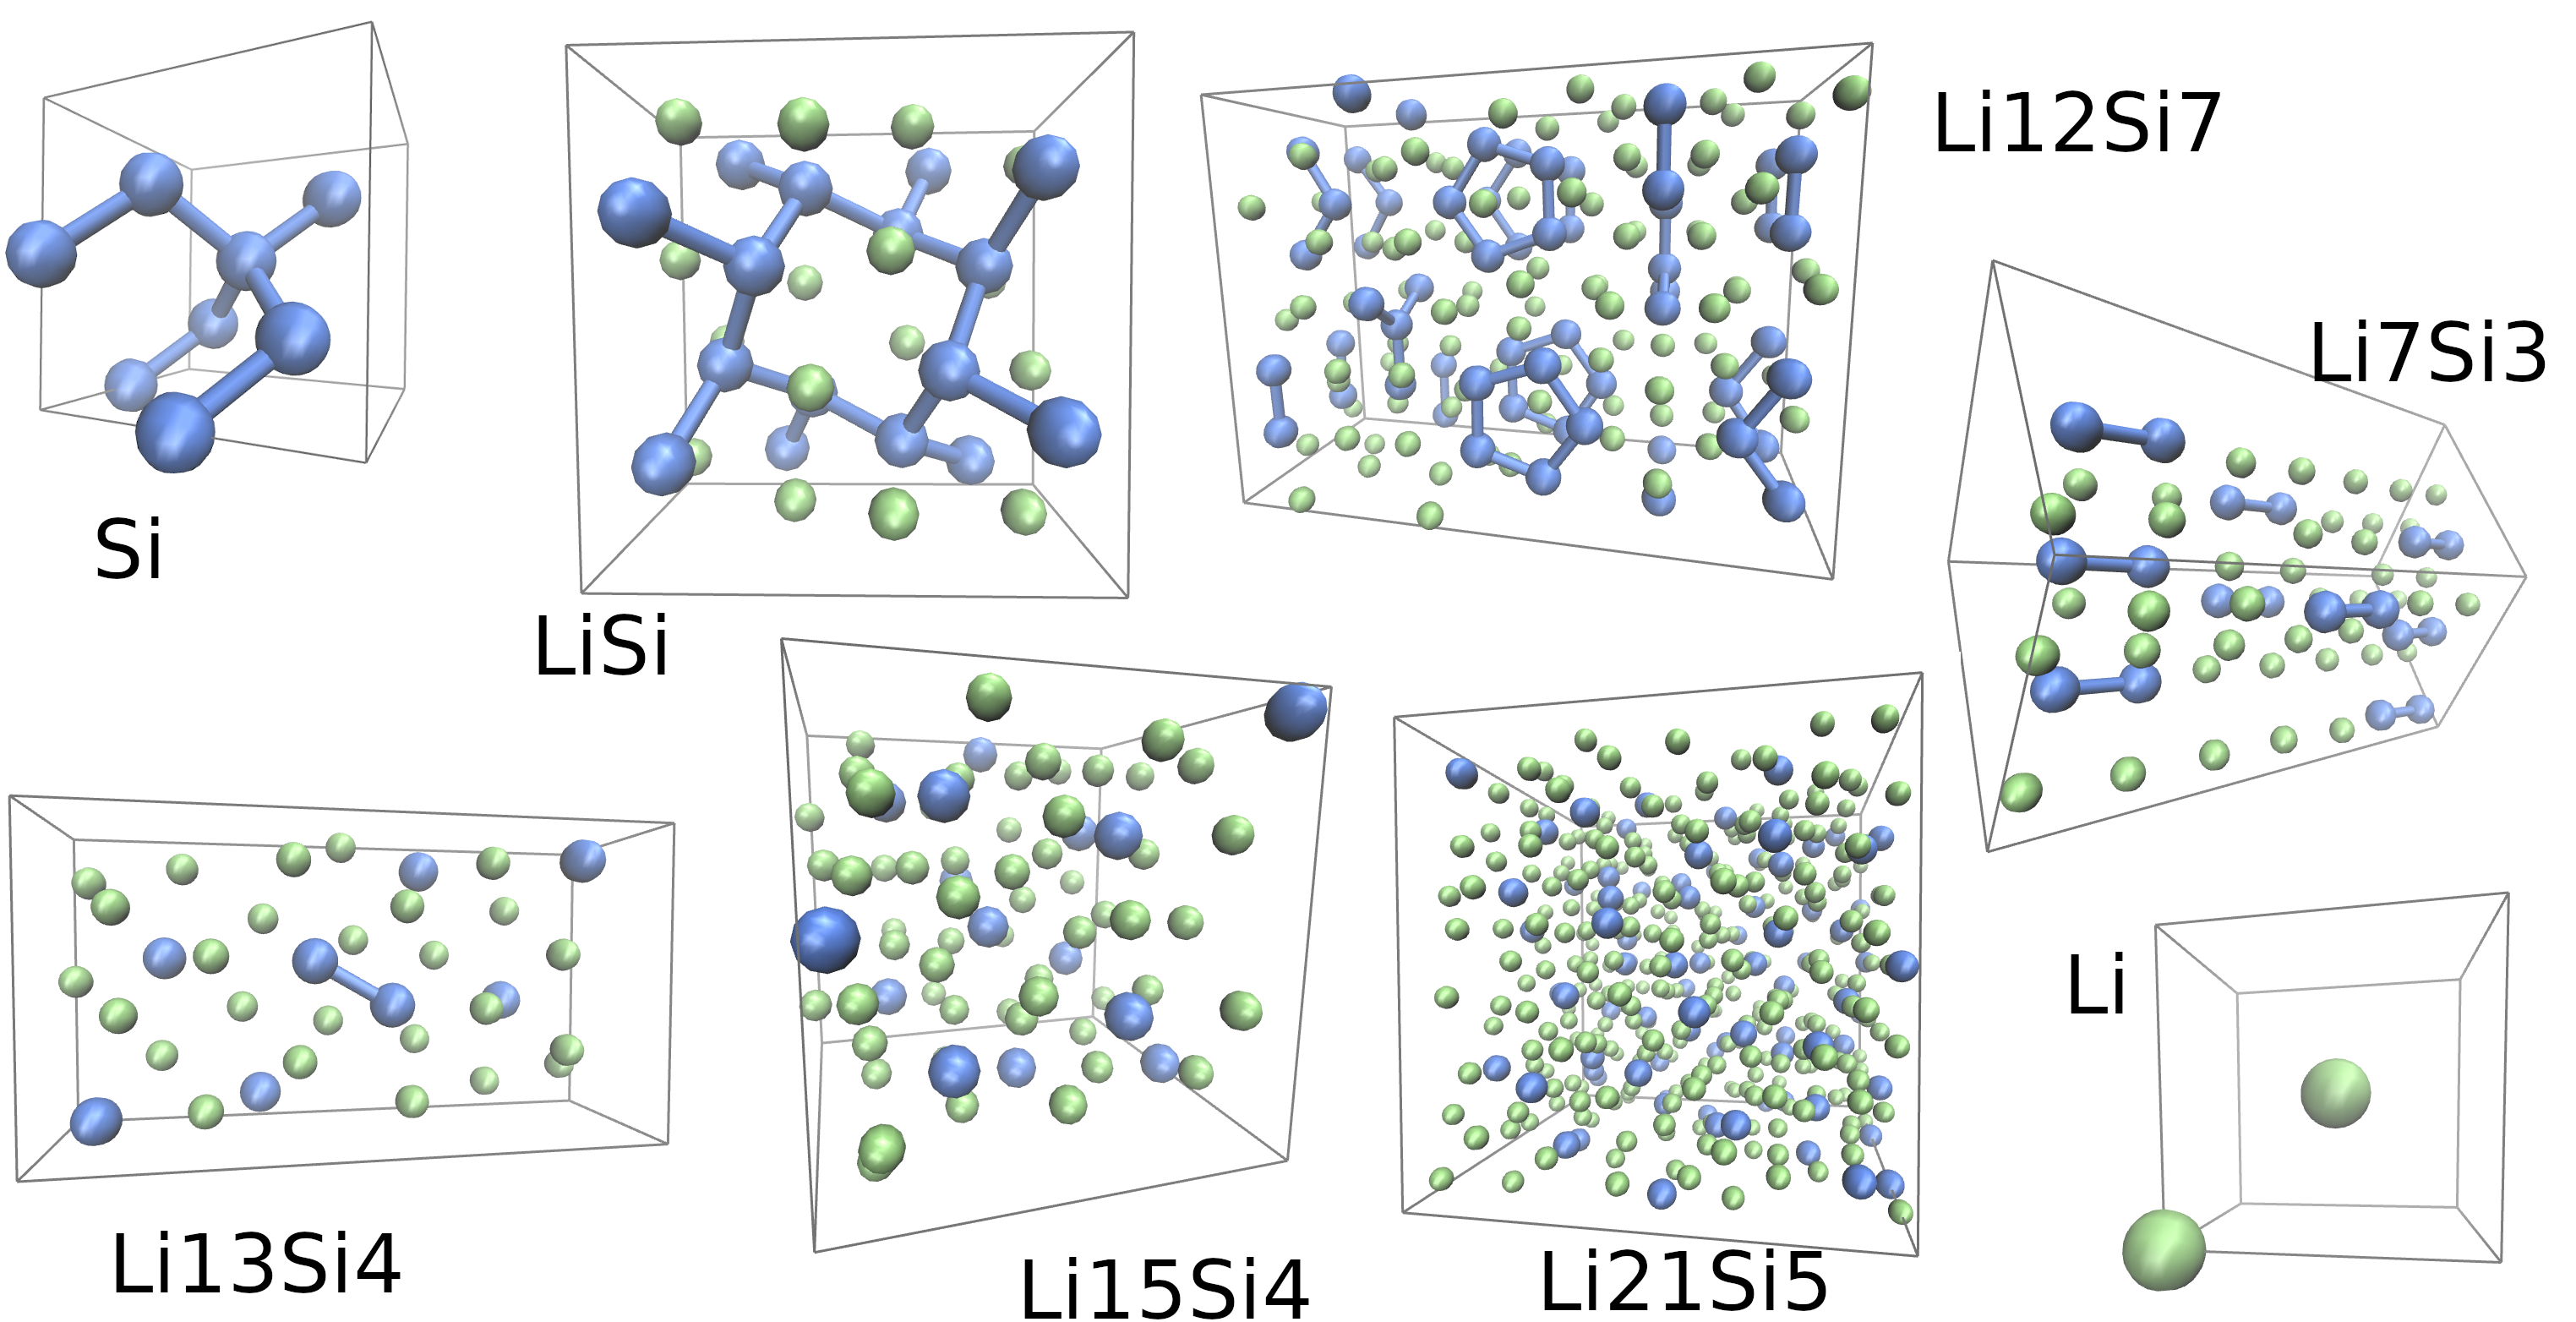
\includegraphics[width=\textwidth]{caracterizacion/cristalinas.png}
    \caption{Estructuras cristalinas de Li-Si. Las estructuras no están a escala 
    entre sí. Los átomos de Si se muestran en azul y los de Li en verde, mientras
    que la celda periódica en gris. Los enlaces de Si-Si están graficados si la 
    distancia entre dos de estos átomos es menor a 2.5\AA.}
    \label{fig:cristalinas}
\end{figure}

\subsection{Protocolo de delitiación}

Para obtener configuraciones iniciales para valores de $x$ distintos a los de las 
cristalinas se siguió un protocolo de delitiación, en el cual se selecciona la 
estructura cristalina más cercana con un valor de $x$ superior al deseado,
se le extrae un átomo de Li de manera aleatoria y se realiza una dinámica en el 
ensamble NPT durante 2 ps para relajar el volumen. Para estas simulaciones se 
utilizó el termostato de Nosé-Hoover ~\cite{nose1984a, nose1984b, hoover1985} a
300.0 K, un barostato a 0.0 atm y un paso temporal de 1 fs utilizando el
software \path{LAMMPS} ~\cite{lammps1, lammps2}. La extracción del átomo de Li y
la simulación en el ensamble NPT fueron repetidas hasta alcanzar una concentración
deseada. Por último, para algunas concentraciones en particular, se seleccionó la
estructura con la menor presión absoluta como estado inicial para la exploración 
acelerada de mínimos locales que se introduce en la siguiente sección.


\section{Exploración acelerada de mínimos locales}

Las simulaciones de MD tienen un gran poder predictivo para el estudio de 
procesos presentes en las baterías de litio, sin embargo, las escalas de tiempo
están limitadas a unos pocos ns o $\mu$s. El número de operaciones que se 
necesita para alcanzar las escalas de tiempo de la operación de una batería 
experimental son prohibitivos, incluso considerando el uso de potenciales 
semi-empíricos como el ReaxFF en supercomputadoras. Como consecuencia de esto,
la MD usual no es suficiente para una exploración del espacio de las fases y las
estructuras de Li-Si observadas van a estar cercanas a las configuraciones 
iniciales mientras que en el sistema real probablemente pueden aparecer otras
configuraciones. Un método simple y poderoso para acelerar la exploración de 
mínimos locales en sistemas moleculares es el templado simulado 
~\cite{kirkpatrick1983}, en el cual básicamente se busca mejorar la exploración
del espacio de las fases en simulaciones de MD utilizando temperaturas altas y
luego reduciéndola progresivamente hasta encontrar un mínimo de energía a 
temperatura ambiente. El templado simulado múltiple (MSA, de sus siglas en inglés 
\textit{Multiple simluated annealing}) utiliza esta idea en distintas copias del 
sistema y fue utilizado para explorar y encontrar distintas estructuras mínimas 
relevantes cercanas al equilibrio ~\cite{hao2015}.

La presente técnica de simulación, exploración acelerada de mínimos locales (AELM,
de sus siglas en inglés \textit{accelerated exploration of local minima}), es 
similar a la MSA pero en vez de calentar y enfriar lentamente el sistema, se 
utiliza un sesgo en la función de energía potencial para sobrepasar las barreras
de energía y luego se realiza una minimización local, con algún minimizador local 
como gradientes conjugados o LBFGS, para encontrar el mínimo. Este método permite 
obtener muchas estructuras con energías mínimas relevantes, que son de interés a 
la hora de estudiar electrodos de Li-Si muy ciclados.

Las aleaciones de Li-Si presentan interacciones fuertes entre los átomos que las
conforman, especialmente en el enlace Si-Si donde la energía de enlace es del
orden de $\approx$2 eV ~\cite{wypych2018handbook}. Se espera que las barreras de 
energía potencial sean de ese orden de magnitud, por lo cual un 
muestreo de una MD a temperatura ambiente parece no ser viable. Para explorar 
ampliamente las distintas configuraciones del sistema, $\mathbf{r}$, se 
transforma la superficie de energía potencial (PES, de sus siglas en inglés 
\textit{potencial energy surface}), $V(\mathbf{r})$, usando un potencial sesgado
\begin{equation}\label{eq:bias}
    V_b(\mathbf{r}) = V(\mathbf{r}) + (\alpha - 1) V(\mathbf{r}) = \alpha V(\mathbf{r}),
\end{equation}
donde $\alpha$ es el factor de compresión. El principal efecto de la ecuación 
\ref{eq:bias} es reducir las barreras de la PES, por lo cual el tiempo de
residencia en estados meta-estables es menor que en el sistema sin sesgar y la 
exploración de configuraciones de sistemas diferentes es más eficiente y 
alcanzada en un tiempo de simulación razonable. El término 
$(\alpha - 1) V(\mathbf{r})$ es usualmente referido como la 
\say{función de sesgo}.

La adición de esta función de sesgo a la PES está en la base del método de 
hiper-dinámica (HD), desarrollado por Voter ~\cite{voter1997HD,voter1997method} 
para acelerar la exploración de un sistema sin perder su dinámica. En una 
simulación típica de HD, para recuperar el promedio de alguna propiedad, la 
configuración muestreada son repesadas por un factor $w$ que involucra una función
exponencial y depende del sesgo aplicado. Debido a que este sistema involucra 
cambios grandes en las energías de interacción, comparado con la energía térmica
$k_BT$, lo que implica que la función exponencial en $w$ toma valores muy grandes,
esto provoca que el procedimiento numérico sea inestable y la recuperación de 
la propiedad de interés, como la energía potencial, no sea posible. Ya que este
capítulo se centra en un estudio estructural de los sistemas, podemos ignorar
el cálculo del tiempo real evolucionado en la simulación. Además, como el 
funcionamiento de las baterías luego se da a temperatura ambiente, es de esperar
que una vez que se alcanza un mínimo local el sistema explore configuraciones
cercanas a este. Por este motivo se aplica el método de gradientes conjugados (CG)
a cada una de las configuraciones de la HD y de esa forma se muestrea la 
multiplicidad de estructuras.

Este método de exploración introducido en esta tesis se asemeja al templado
simulado, aunque el objetivo es explorar muchas estructuras diferentes en vez de 
encontrar el mínimo global. El templado simulado fue utilizado anteriormente
con este mismo objetivo, Hao \textit{et al.} utilizó la técnica MSA para obtener
distintas estructuras de mínima energía de péptidos ~\cite{hao2015}. En este 
método AELM se usa HD en vez de temperaturas altas para favorecer la exploración,
y se realizan múltiples minimizaciones por CG en vez de simular un enfriado. 


\section{Resultados}

Las simulaciones aceleradas fueron llevadas a cabo en el ensamble NVT a 300.0 K
con un termostato de Langevin ~\cite{schneider1978} utilizando una versión 
modificada de \path{GEMS} ~\cite{gems}. A cada estructura se le realizó una 
minimización de gradientes conjugados con el software \path{LAMMPS} 
~\cite{lammps1, lammps2}. El tamaño de los sistemas y la cantidad de estructuras 
utilizadas para obtener los siguiente resultados se presentan en la tabla 
\ref{t:siminfo}.
\begin{table}[h]
    \centering
    \caption{Información del conjunto de datos.}
    \setlength\extrarowheight{2pt}\stackon{%
    \begin{tabular}{c c c c c c c c}
        \toprule
        \thead{\normalsize\bfseries $x$ en Li$_{x}$Si} & 
        \thead{\normalsize\bfseries N$_{Li}$} & 
        \thead{\normalsize\bfseries N$_{Si}$} &
        \thead{\normalsize\bfseries N$_{estructuras}$} & 
        \thead{\normalsize\bfseries E$_{mean}$ / N$_T$ [eV]} & 
        \thead{\normalsize\bfseries E$_{std}$ / N$_T$ [eV]} & 
        \thead{\normalsize\bfseries $\sqrt{kT}$ / N$_T$ [eV]} \\
        \midrule
        0.21 & 140 & 667 & 774 & -4.399 & 0.003 & 0.0002 \\
        0.62 & 416 & 670 & 1665 & -4.002 & 0.005 & 0.0001 \\
        1.25 & 839 & 671 & 1224 & -3.521 & 0.004 & 0.0001 \\
        1.71 & 1152 & 672 & 2132 & -3.286 & 0.002 & 0.0001 \\
        2.17 & 693 & 319 & 1699 & -3.126 & 0.002 & 0.0002 \\
        2.71 & 865 & 319 & 1504 & -2.964 & 0.002 & 0.0001 \\
        3.25 & 1040 & 320 & 1464 & -2.856 & 0.003 & 0.0001 \\
        3.75 & 1080 & 288 & 2660 & -2.777 & 0.002 & 0.0001 \\
        4.20 & 1344 & 320 & 1600 & -2.717 & 0.001 & 0.0001 \\
        \bottomrule
    \end{tabular}
    }{}
    \label{t:siminfo}
\end{table}

\begin{figure}[th]
    \centering
    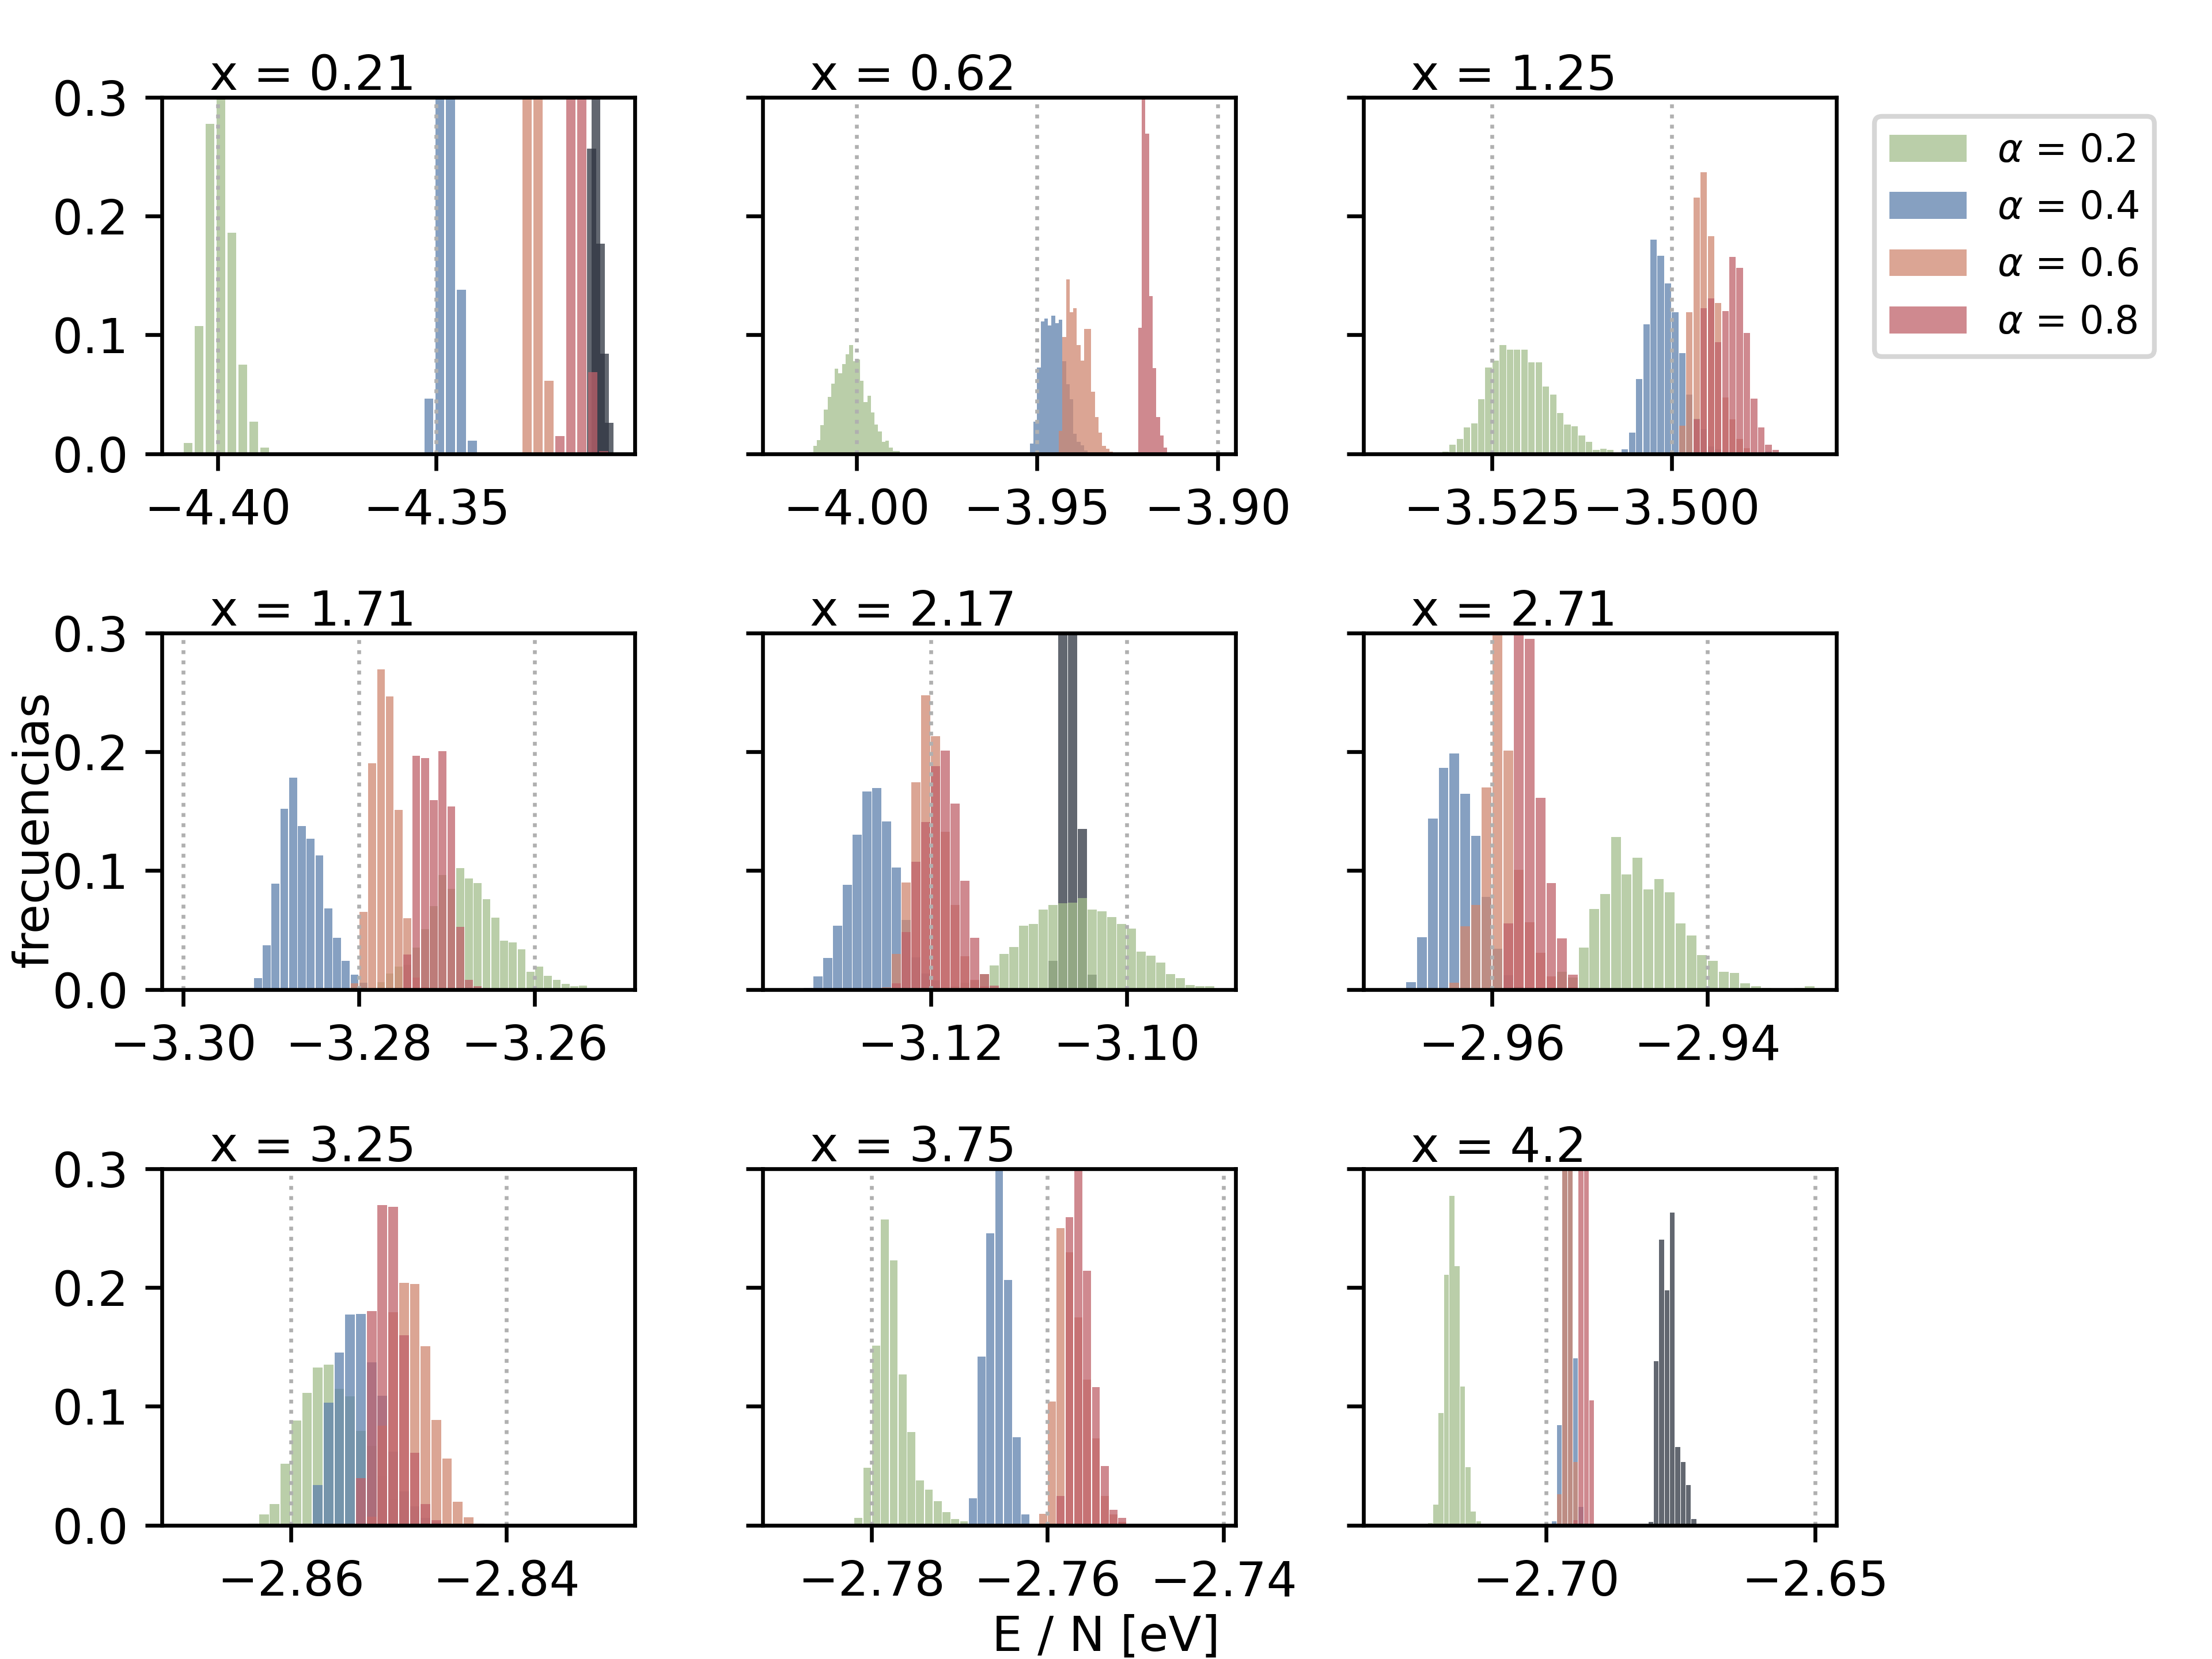
\includegraphics[width=\textwidth]{caracterizacion/energias.png}
    \caption{Histogramas correspondientes a la energía potencial de las 
    estructuras obtenidas con el método AELM, con distintos valores de $\alpha$
    en la ecuación \ref{eq:bias}, para cada composición de Li$_x$Si estudiada.}
    \label{fig:energias}
\end{figure}
La figura \ref{fig:energias} muestra los histogramas para las energías mínimas
de las estructuras de Li$_x$Si obtenidas con el método AELM para los valores de
$x$ estudiados y distintos valores de compresión $\alpha$. En cada fila hay un 
histograma de energías representativo para las estructuras de concentración 
cercana, por lo cual en el análisis sólo son nombradas algunas de estas 
concentraciones. Para el primer caso, donde $x = 0.21$, se puede apreciar como el 
uso de valores más pequeños de $\alpha$ permite que estructuras con menor energía 
sean encontradas. El principal efecto de este factor $\alpha$ sobre la PES es la 
disminución de sus barreras de energía, mejorando la exploración del espacio de 
las fases. Este efecto se vuelve más drástico a medida que el valor de $\alpha$ 
tiende a cero. Para estas concentraciones representativas también se realizaron 
simulaciones de MD usuales, es decir, con un valor de $\alpha = 1$, estas no 
pueden sobrepasar las barreras de energías durante el tiempo simulado. El sistema 
permanece cercano al mínimo local asociado a la configuración inicial. Por otro 
lado, el uso de $\alpha = 0.2$ en el método de AELM resulta en un acceso rápido
a estructuras de energías menores. Un comportamiento similar se observa para 
$x = 2.17$, sin embargo, en este caso el valor más pequeño de $\alpha$ tiende a 
encontrar energías más altas que los otros casos, dando lugar a una distribución
similar a la de MD ordinaria pero con mayores fluctuaciones. Esto probablemente 
se deba a una exploración demasiado extensa, donde el sistema difunde a través
de una gran región del espacio de las fases y las minimizaciones múltiples de 
CG no son capaces de encontrar mínimos de menor energía. Por último, para la 
concentración más alta, correspondiente a un valor de $x = 4.2$, las simulaciones 
de AELM con un valor de $\alpha = 0.2$ son capaces de encontrar estructuras que 
reducen fuertemente la energía potencial del sistema. 

\begin{figure}[t]
    \centering
    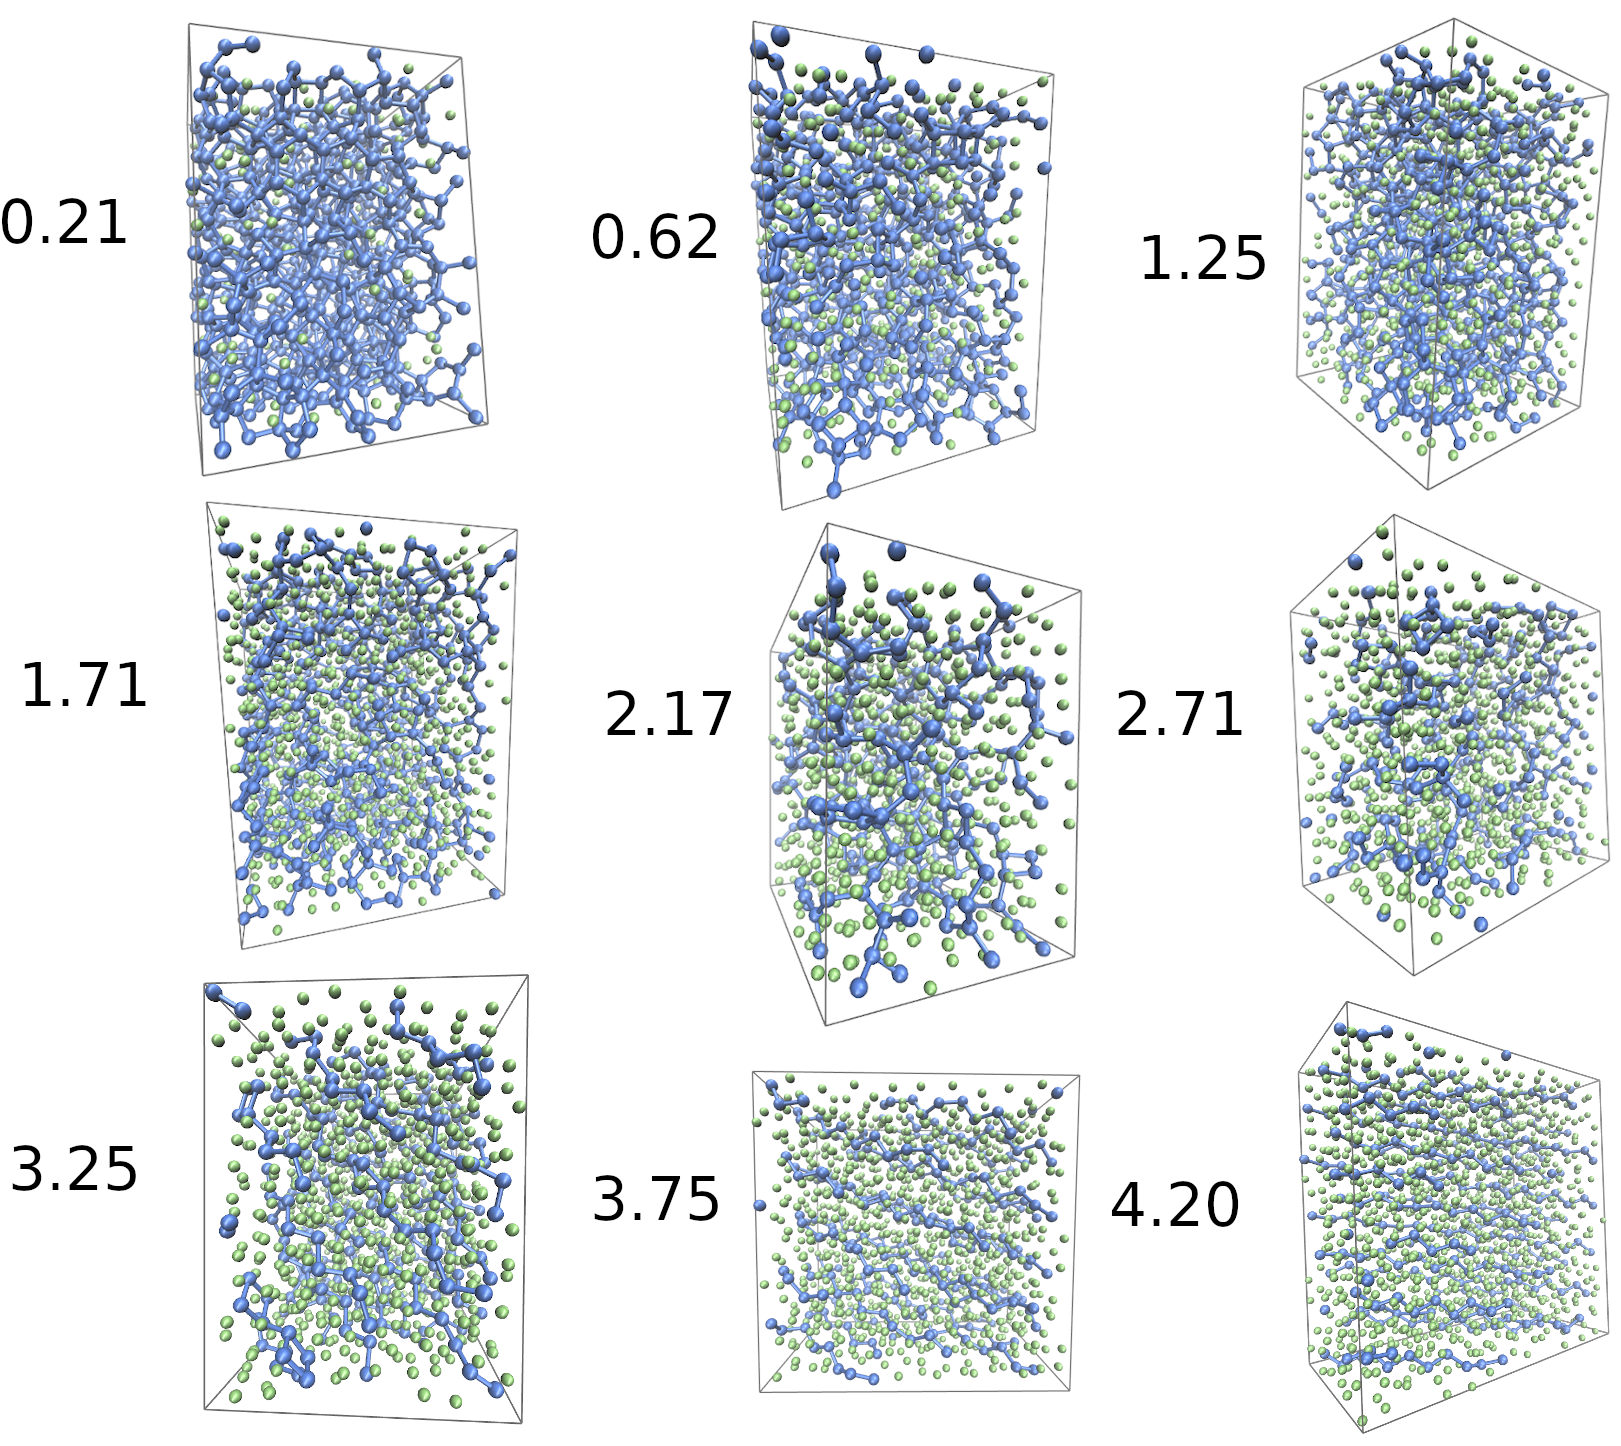
\includegraphics[width=\textwidth]{caracterizacion/amorfas.png}
    \caption{Configuración amorfa representativa de cada valor de $x$. Los átomos
    de Si se muestran en azul mientras que los de Li en verde.}
    \label{fig:amorfas}
\end{figure}
De los histogramas de la figura \ref{fig:energias} se seleccionan los factores 
de aceleración más óptimos, es decir que producen energías menores, para obtener
las propiedades estructurales que se discuten a continuación. Para estos valores
se muestra una estructura representativa a cada composición en la figura 
\ref{fig:amorfas}. Para $x = 0.21$ puede verse que la red amorfa de silicio
permanece con su estructura tetraédrica desordenada. Algunos enlaces Si-Si 
comienzan a romperse a medida que la concentración de litio aumenta, como puede
verse para las estructuras cercanas a $x = 2.17$. Por último, para las 
concentraciones más altas de litio, se alcanzan estructuras que involucran 
cadenas unidimensionales periódicas de silicio. Una estructura similar ha sido 
reportada por Ostadhossein \textit{et al.} ~\cite{ostadhossein2015}. En las 
próximas secciones se caracterizan dichas estructuras.

\subsection{Comportamiento electroquímico}

\subsubsection{Cambio de volumen fraccionario}

El cambio de volumen fraccionario puede definirse utilizando una normalización 
relativa al número de átomos de Si en la estructura de acuerdo a
\begin{equation}\label{eq:fvc}
    fvc = \frac{N_{Si}}{V_{Si}} \left( \frac{V_{Si,x}}{N_{Si,x}} - \frac{V_{Si}}{N_{Si}} \right),
\end{equation}
donde $V_{Si}$ y $N_{Si}$ son el volumen y el número de átomos de Si en la celda
unidad de c-Si, $V_{Si,x}$ y $N_{Si,x}$ son el volumen y el número de átomos de Si
en la celda de simulación para el valor correspondiente de $x$. En la figura
\ref{fig:fvc} se muestran los valores calculados a partir de la ecuación 
\ref{eq:fvc} para las distintas estructuras de Li$_x$Si estudiadas. En la misma 
se comparan los valores obtenidos con datos experimentales de AFM (\textit{atomic 
force microscopy}, sus siglas en inglés) medidos por Beaulieu \textit{et al.} 
~\cite{beaulieu2003} y con predicciones de DFT con un cambio volumétrico fijo 
utilizado por Chevrier y Dahn ~\cite{chevrier2009}. Los mismos muestran que el
potencial ReaxFF proporciona una tendencia correcta, tanto cualitativa como 
cuantitativamente.
\begin{figure}[th]
    \centering
    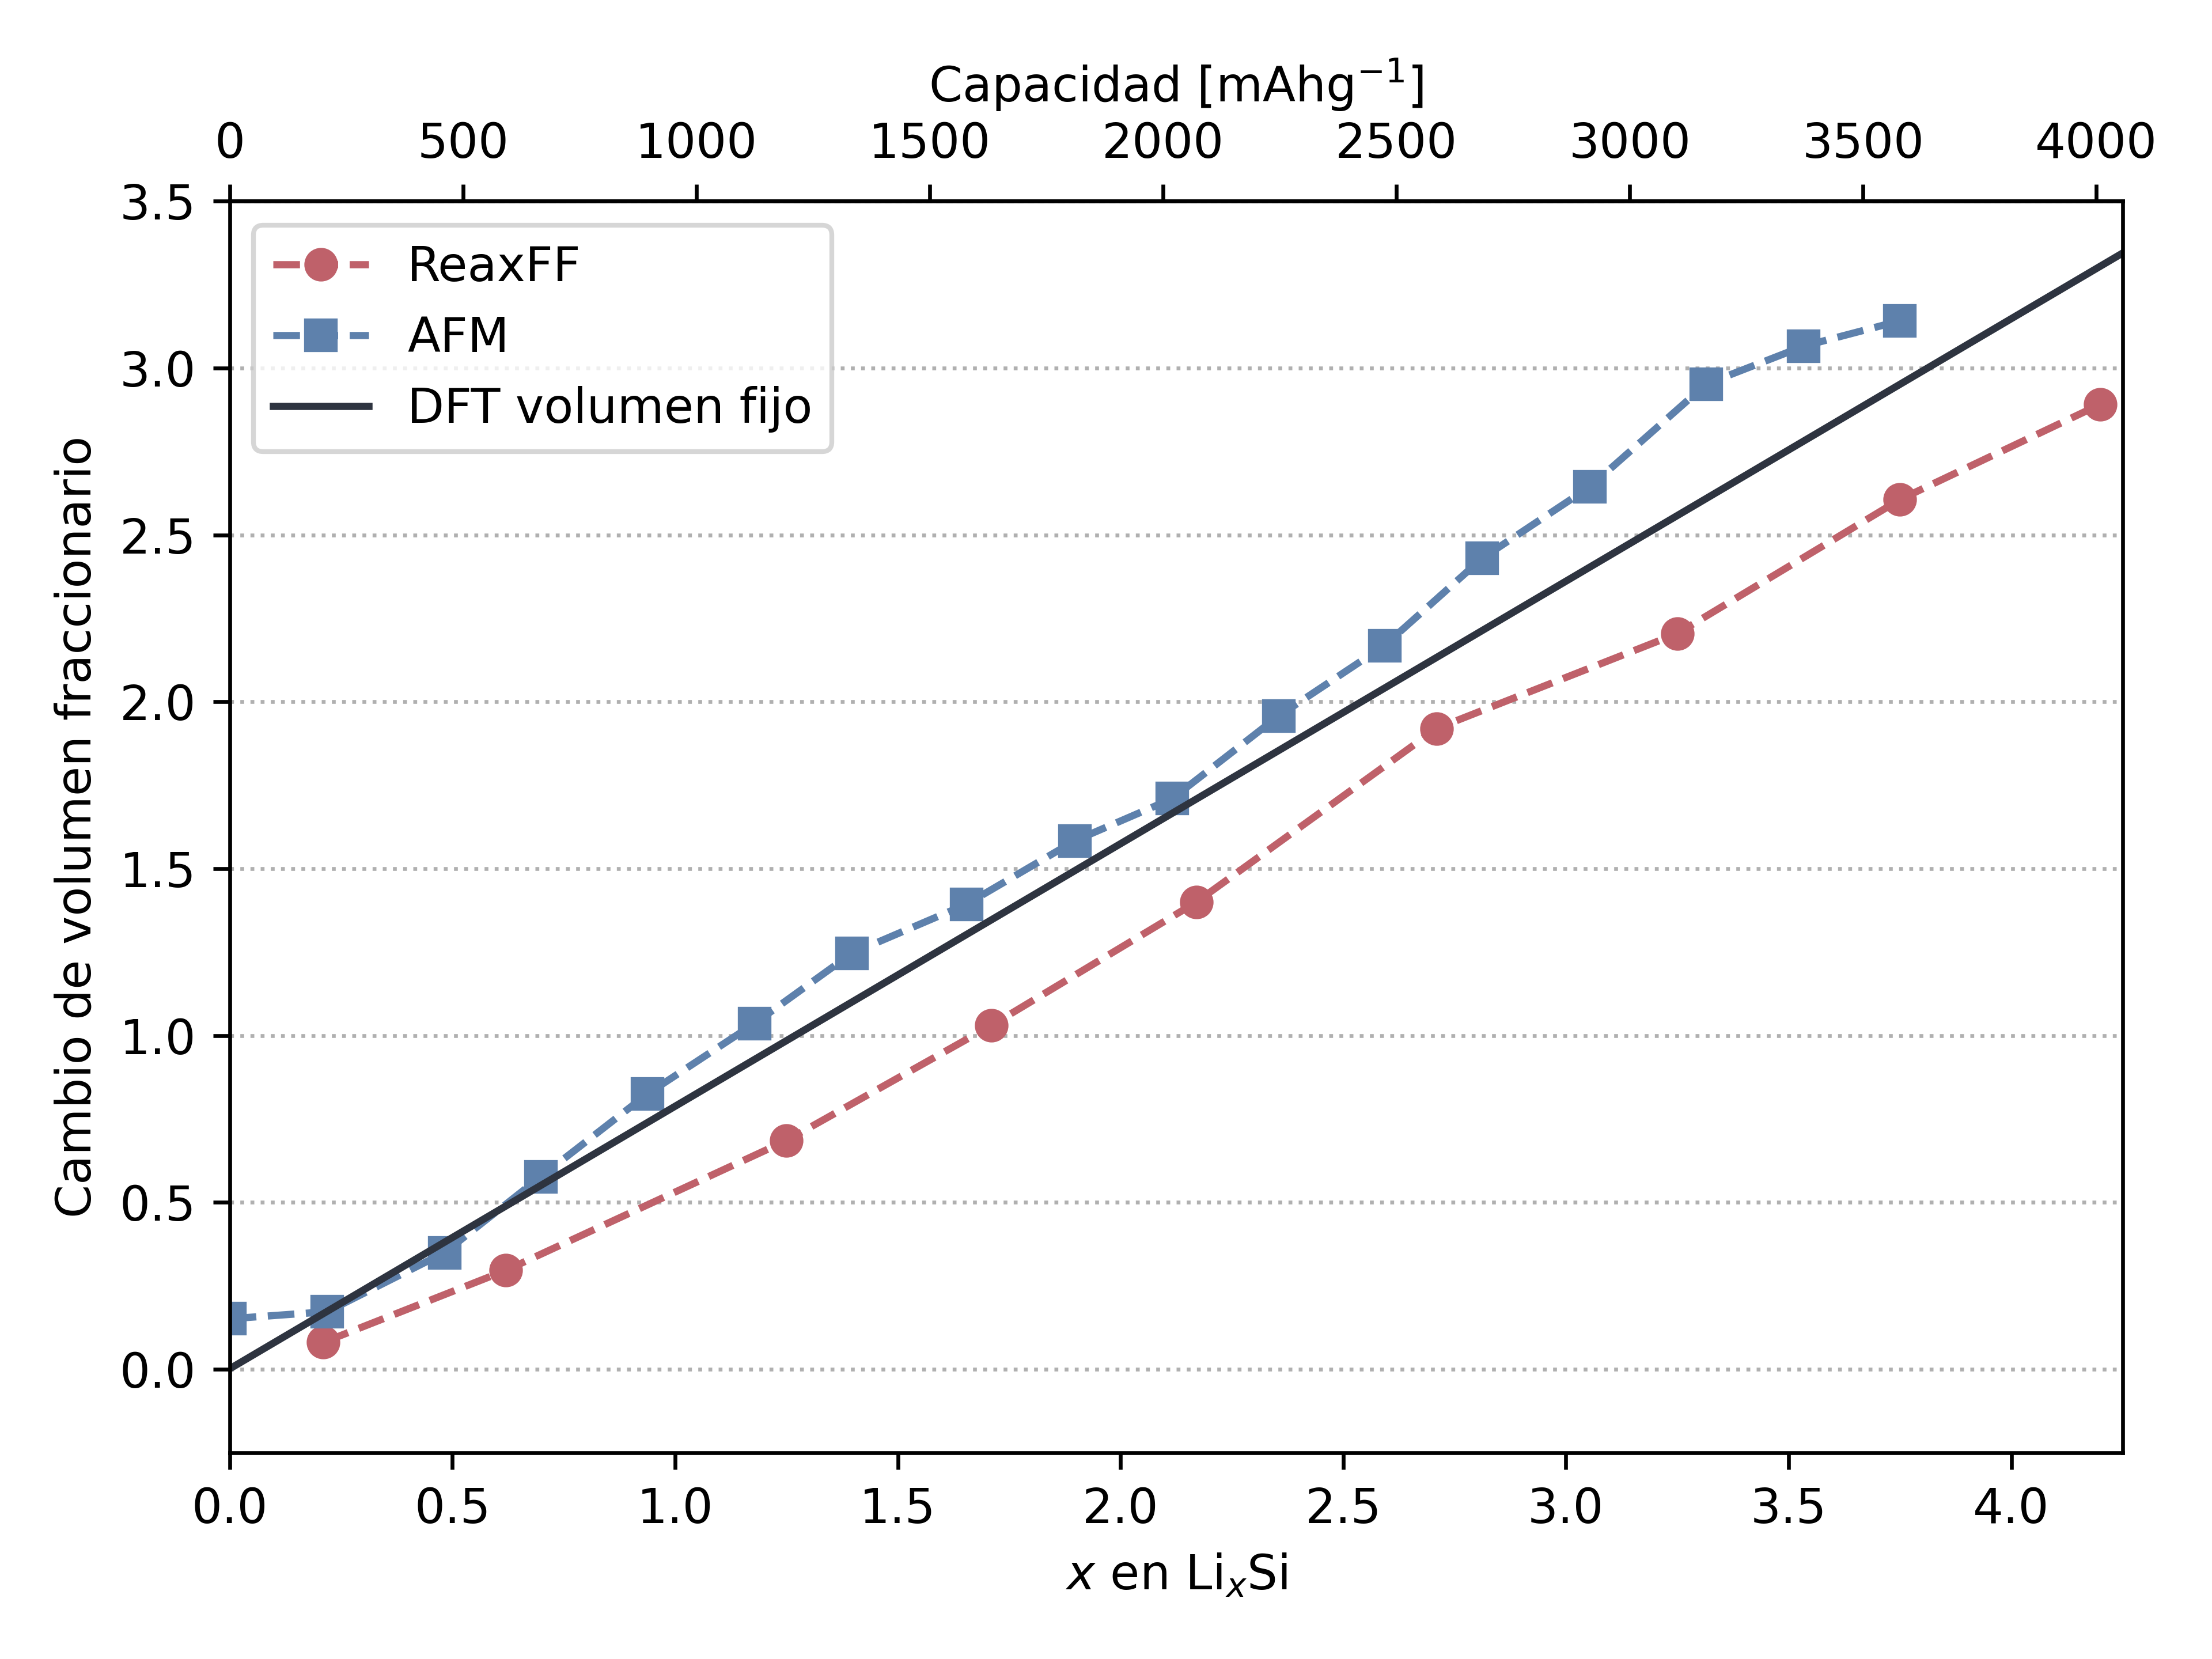
\includegraphics[width=0.8\textwidth]{caracterizacion/fvc.png}
    \caption{Cambio de volumen fraccionario en función de la composición de la 
    aleación. Los valores experimentales de AFM se muestran con cuadrados azules, 
    la línea recta se corresponde con cálculos de DFT y los círculos rojos son 
    resultados de este trabajo.}
    \label{fig:fvc}
\end{figure}

\subsubsection{Voltaje}

\begin{table}[h]
    \centering
    \caption{Energías de formación obtenidas a través de la ecuación \ref{eq:fe}}
    \setlength\extrarowheight{2pt}\stackon{%
    \begin{tabular}{c c c}
        \toprule
        \thead{\normalsize\bfseries x en Li$_x$Si} & 
        \thead{\normalsize\bfseries Energía de\\\normalsize\bfseries formación [eV]} & 
        \thead{\normalsize\bfseries Desviación\\\normalsize\bfseries estándar [eV]} \\
        \midrule
        0.21  &  0.5027  &  0.0037 \\
        0.62  &  0.1206  &  0.0074 \\
        1.25  & -0.1160  &  0.0096 \\
        1.71  & -0.2358  &  0.0065 \\
        2.17  & -0.3551  &  0.0075 \\
        2.71  & -0.4098  &  0.0072 \\
        3.25  & -0.5187  &  0.0126 \\
        3.75  & -0.6202  &  0.0097 \\
        4.20  & -0.6995  &  0.0075 \\
        \bottomrule
    \end{tabular}
    }{}
    \label{t:fe}
\end{table}
Las energías obtenidas pueden ser utilizadas para evaluar el funcionamiento del 
modelo para predecir propiedades electroquímicas, como fue sugerido por Chevrier
y Dahn ~\cite{chevrier2009}. Primero, se define la energía de formación de las 
distintas estructuras amorfas como
\begin{equation}\label{eq:fe}
    E_f(x) = E_{Li_xSi} - (x E_{Li} + E_{Si}),
\end{equation}
donde $E_{Li_xSi}$ es la energía de la aleación Li$_x$Si por átomo de Si, E$_{Li}$
y E$_{Si}$ son las energías cohesivas de Li y Si en sus fases cristalinas. Usando
la ecuación \ref{eq:fe} como aproximación a la energía de formación de Gibbs, el 
potencial \textit{versus} Li metálico de Li$_x$Si puede obtenerse a partir de
\begin{equation}\label{eq:voltaje}
    V(x) = - \frac{dE_f(x)}{dx},
\end{equation}
donde $V$ es el potencial. Los datos obtenidos así pueden compararse con valores
experimentales y computacionales previos. Las energías de formación calculadas
a partir de la ecuación \ref{eq:fe} se muestran en la tabla \ref{t:fe}. 
Si se realiza un \textit{spline} a estos valores, mostrados en el recuadro de la
figura \ref{fig:voltaje}, se obtienen los valores de $V(x)$ a partir de la ecuación
\ref{eq:voltaje}, que se grafican en función de la composición en la figura 
\ref{fig:voltaje} con una línea roja. Para comparar, se incluye en la misma figura
las curvas experimentales medidas para la litiación y la delitiación de silicio
amorfo ~\cite{hatchard2004} y la curva teórica de cálculos de primeros principios 
~\cite{chevrier2009}. Se puede afirmar que los resultados obtenidos con el ReaxFF 
son satisfactorios.
\begin{figure}[th]
    \centering
    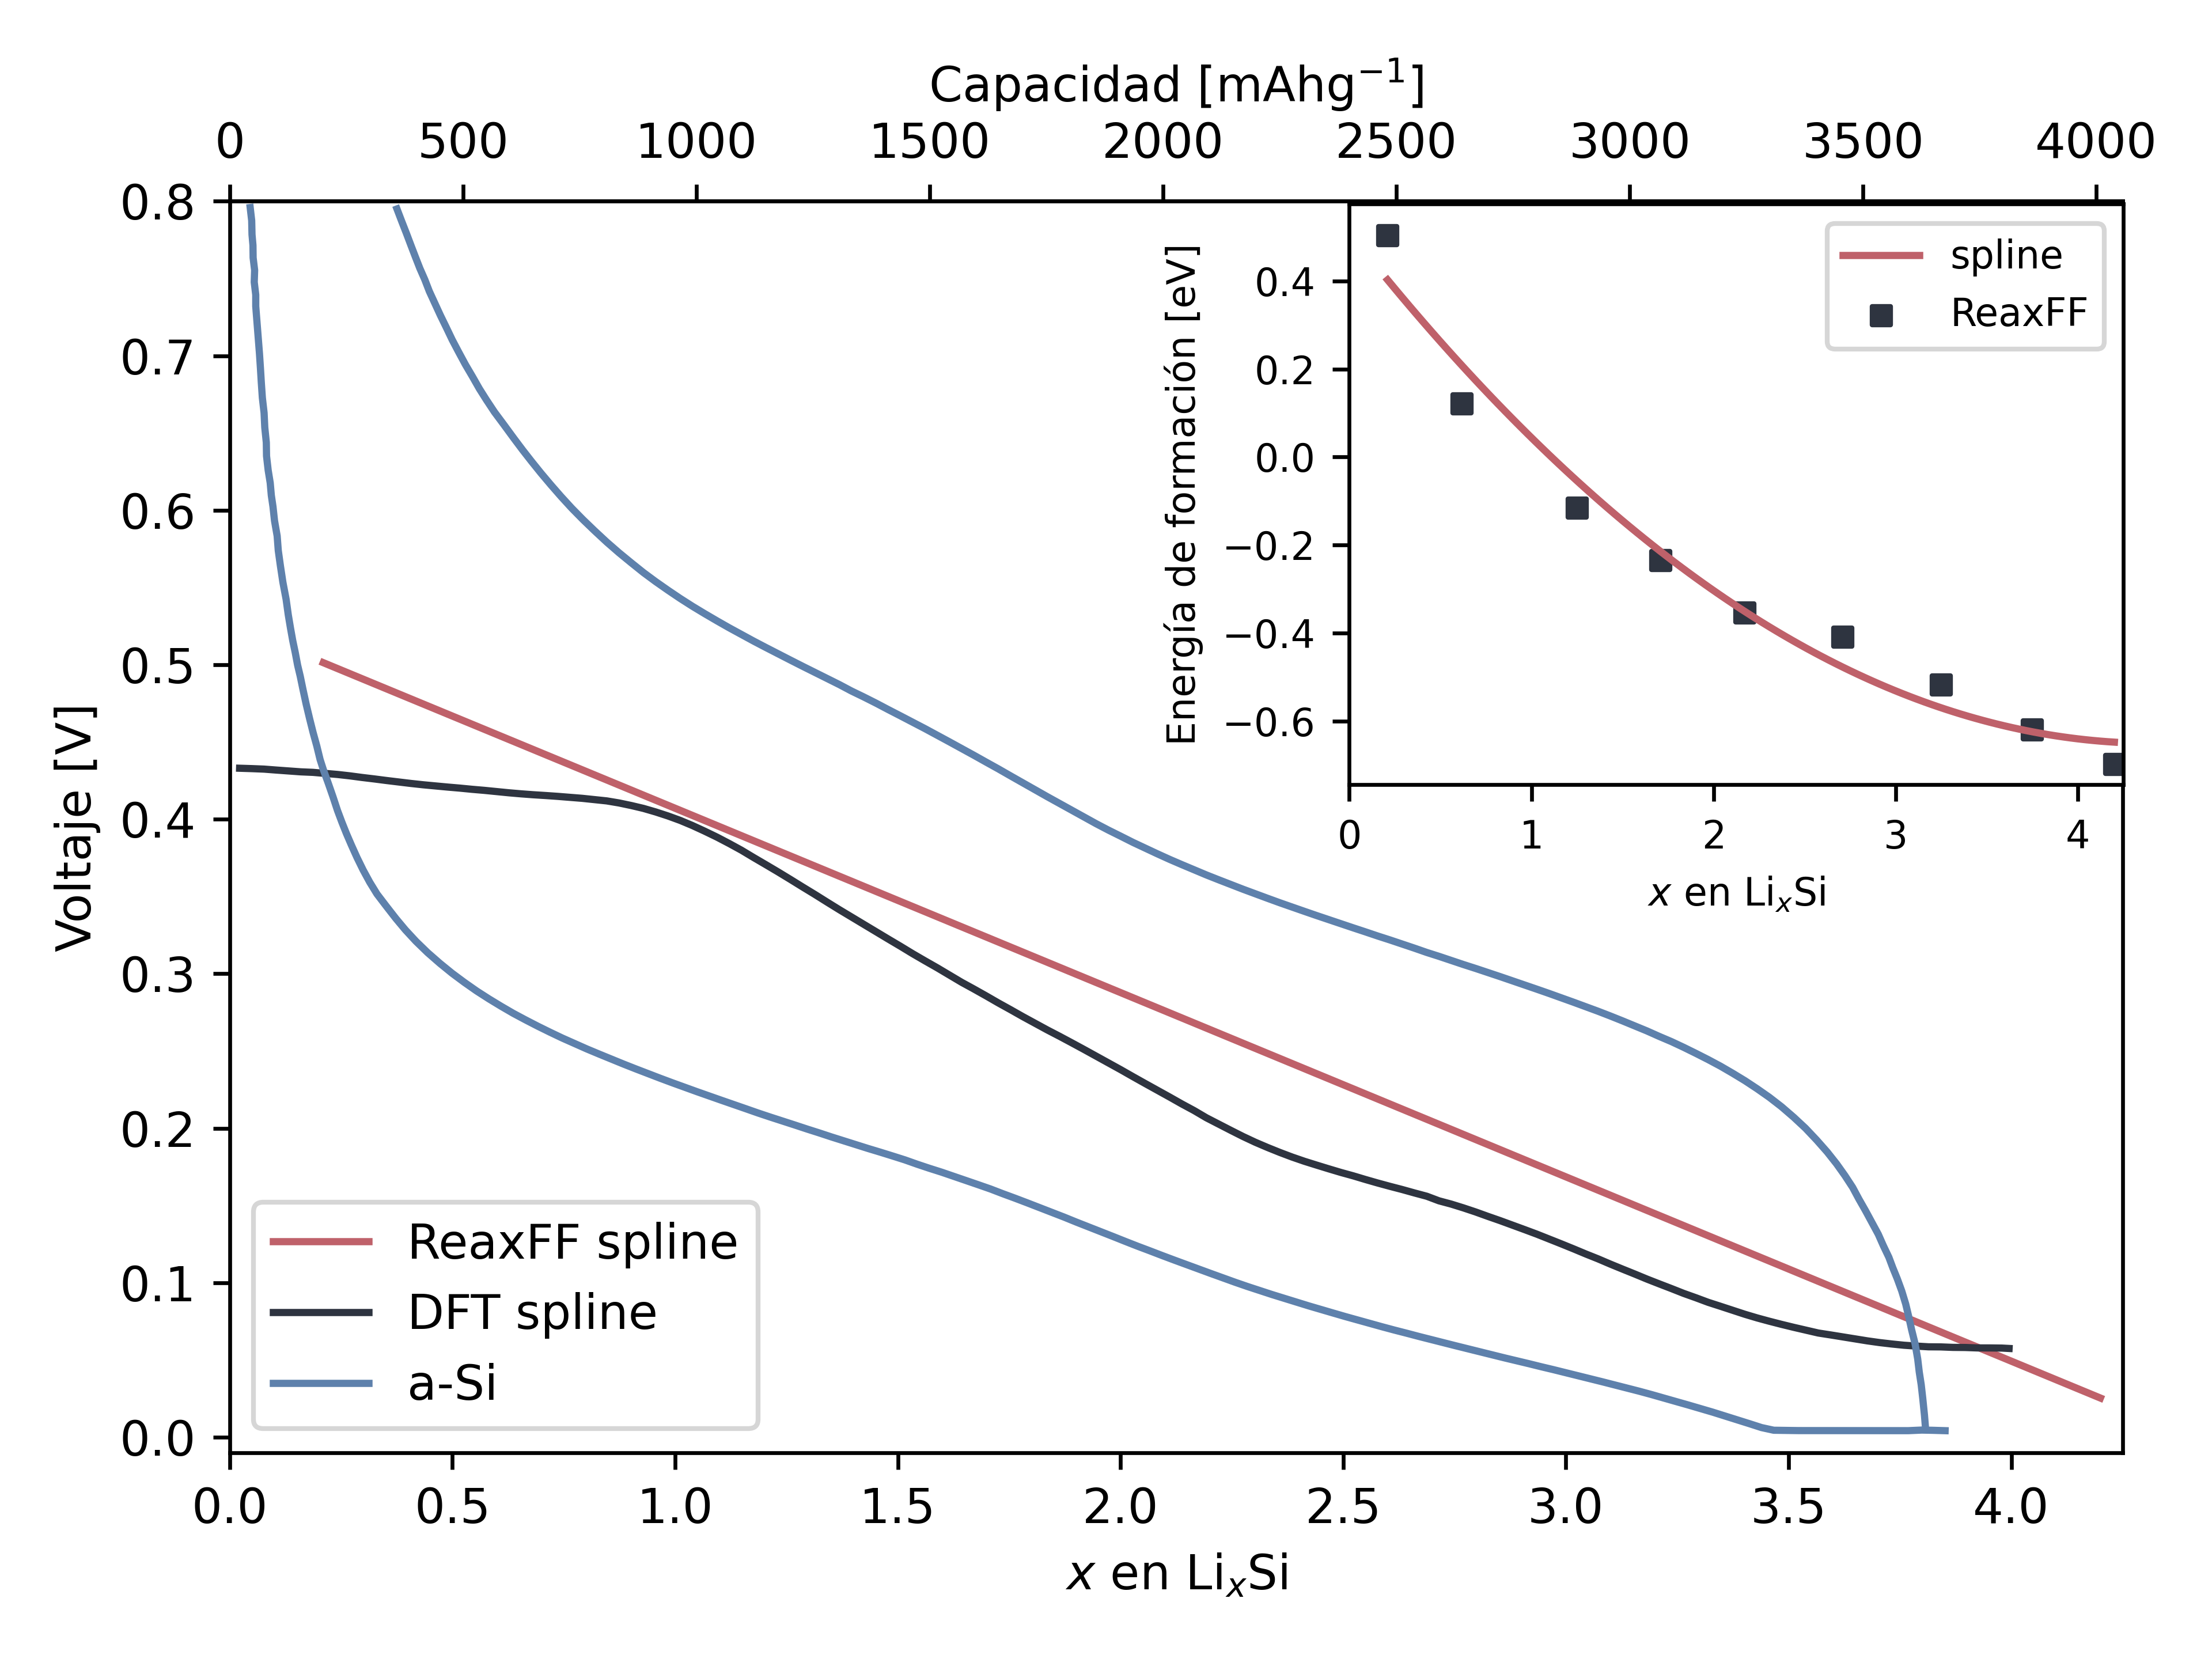
\includegraphics[width=0.8\textwidth]{caracterizacion/voltaje.png}
    \caption{Curvas potencial-concentración para la litiación de ánodos de Si.
    La línea negra corresponde a cálculos de DFT, las líneas azules a 
    curvas medidas experimentalmente en la litiación de Si amorfo y la línea 
    roja es la derivada del \textit{spline} ajustado a los datos de la energía 
    de formación obtenidos con el ReaxFF, presentados en el recuadro.}
    \label{fig:voltaje}
\end{figure}

\subsection{Distribución radial de a pares}

La distribución radial de a pares, introducida en la sección \ref{s:observables},
puede ser utilizada para describir la estructura de materiales amorfos. Para el 
caso de sistemas que están conformados por más de un elemento se pueden analizar 
las distribuciones radiales de a pares parciales ~\cite{lamparter1995}, donde la 
$g_{ij}(r)$ representa la RDF de los átomos $j$ a una distancia $r$ alrededor de 
los átomos centrales $i$, y que es lo mismo que considerar $g_{ji}(r)$. Las 
figuras \ref{fig:rdf-LiLi}, \ref{fig:rdf-SiSi}, \ref{fig:rdf-SiLi} muestran los
resultados obtenidos para las RDF de Li-Li, Si-Si y Si-Li, respectivamente. En
cada una de ellas se analizan los cambios en la estructura que se dan para los
distintos valores de $x$ en Li$_x$Si estudiados, las curvas se calculan sobre las
estructuras minimizadas de la HD.

\begin{figure}[h!]
    \centering
    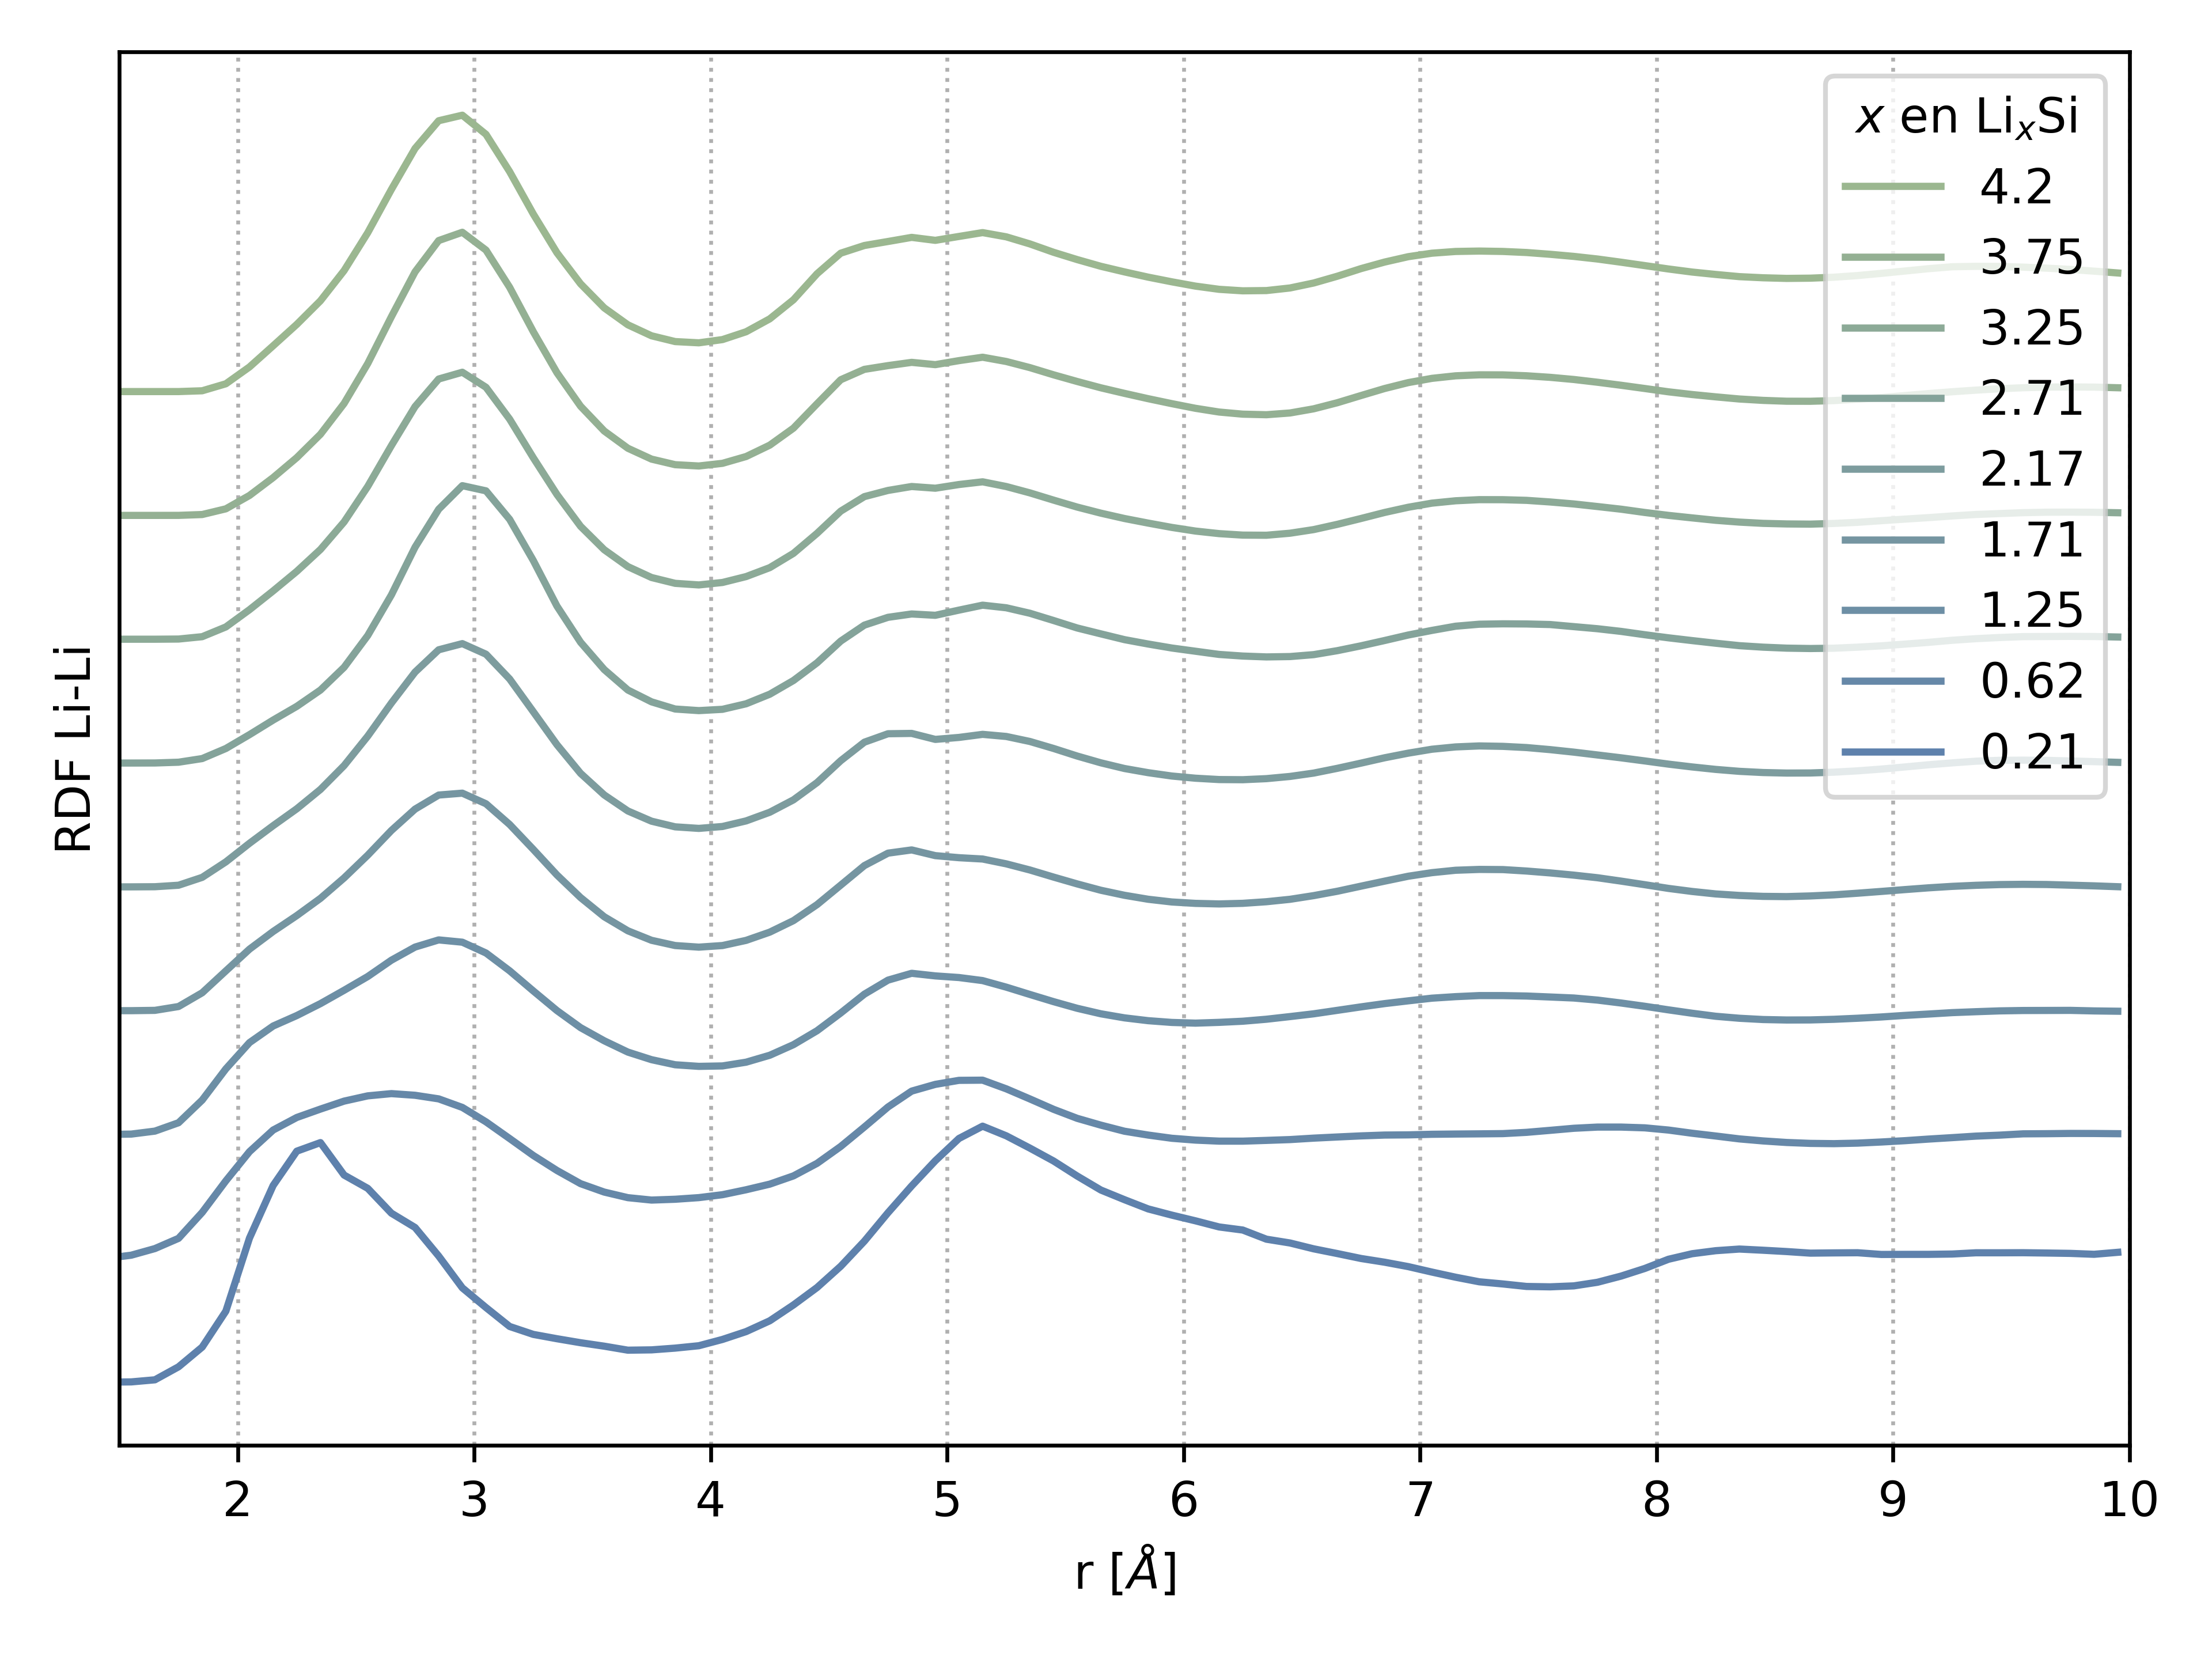
\includegraphics[width=0.8\textwidth]{caracterizacion/rdf-LiLi.png}
    \caption{Distribución radial de a pares para Li-Li de las estructuras 
    minimizadas. Cada curva se corresponde con un valor de concentración 
    distinto.}
    \label{fig:rdf-LiLi}
\end{figure}
Lo más relevante a destacar de la RDF$_{Li-Li}$ es que su primer pico comienza 
centrado en 2.45 \AA\ para las concentraciones de iones de Li más bajas y que 
luego dicho pico aumenta su posición a distancias más grandes a medida que aumenta
$x$ hasta permanecer en 2.95 \AA\ para $x$ mayores a 1.71. La altura de este pico
aumenta en un 50\% luego de la litiación completa, relativa a la menor 
concentración.

\begin{figure}[h!]
    \centering
    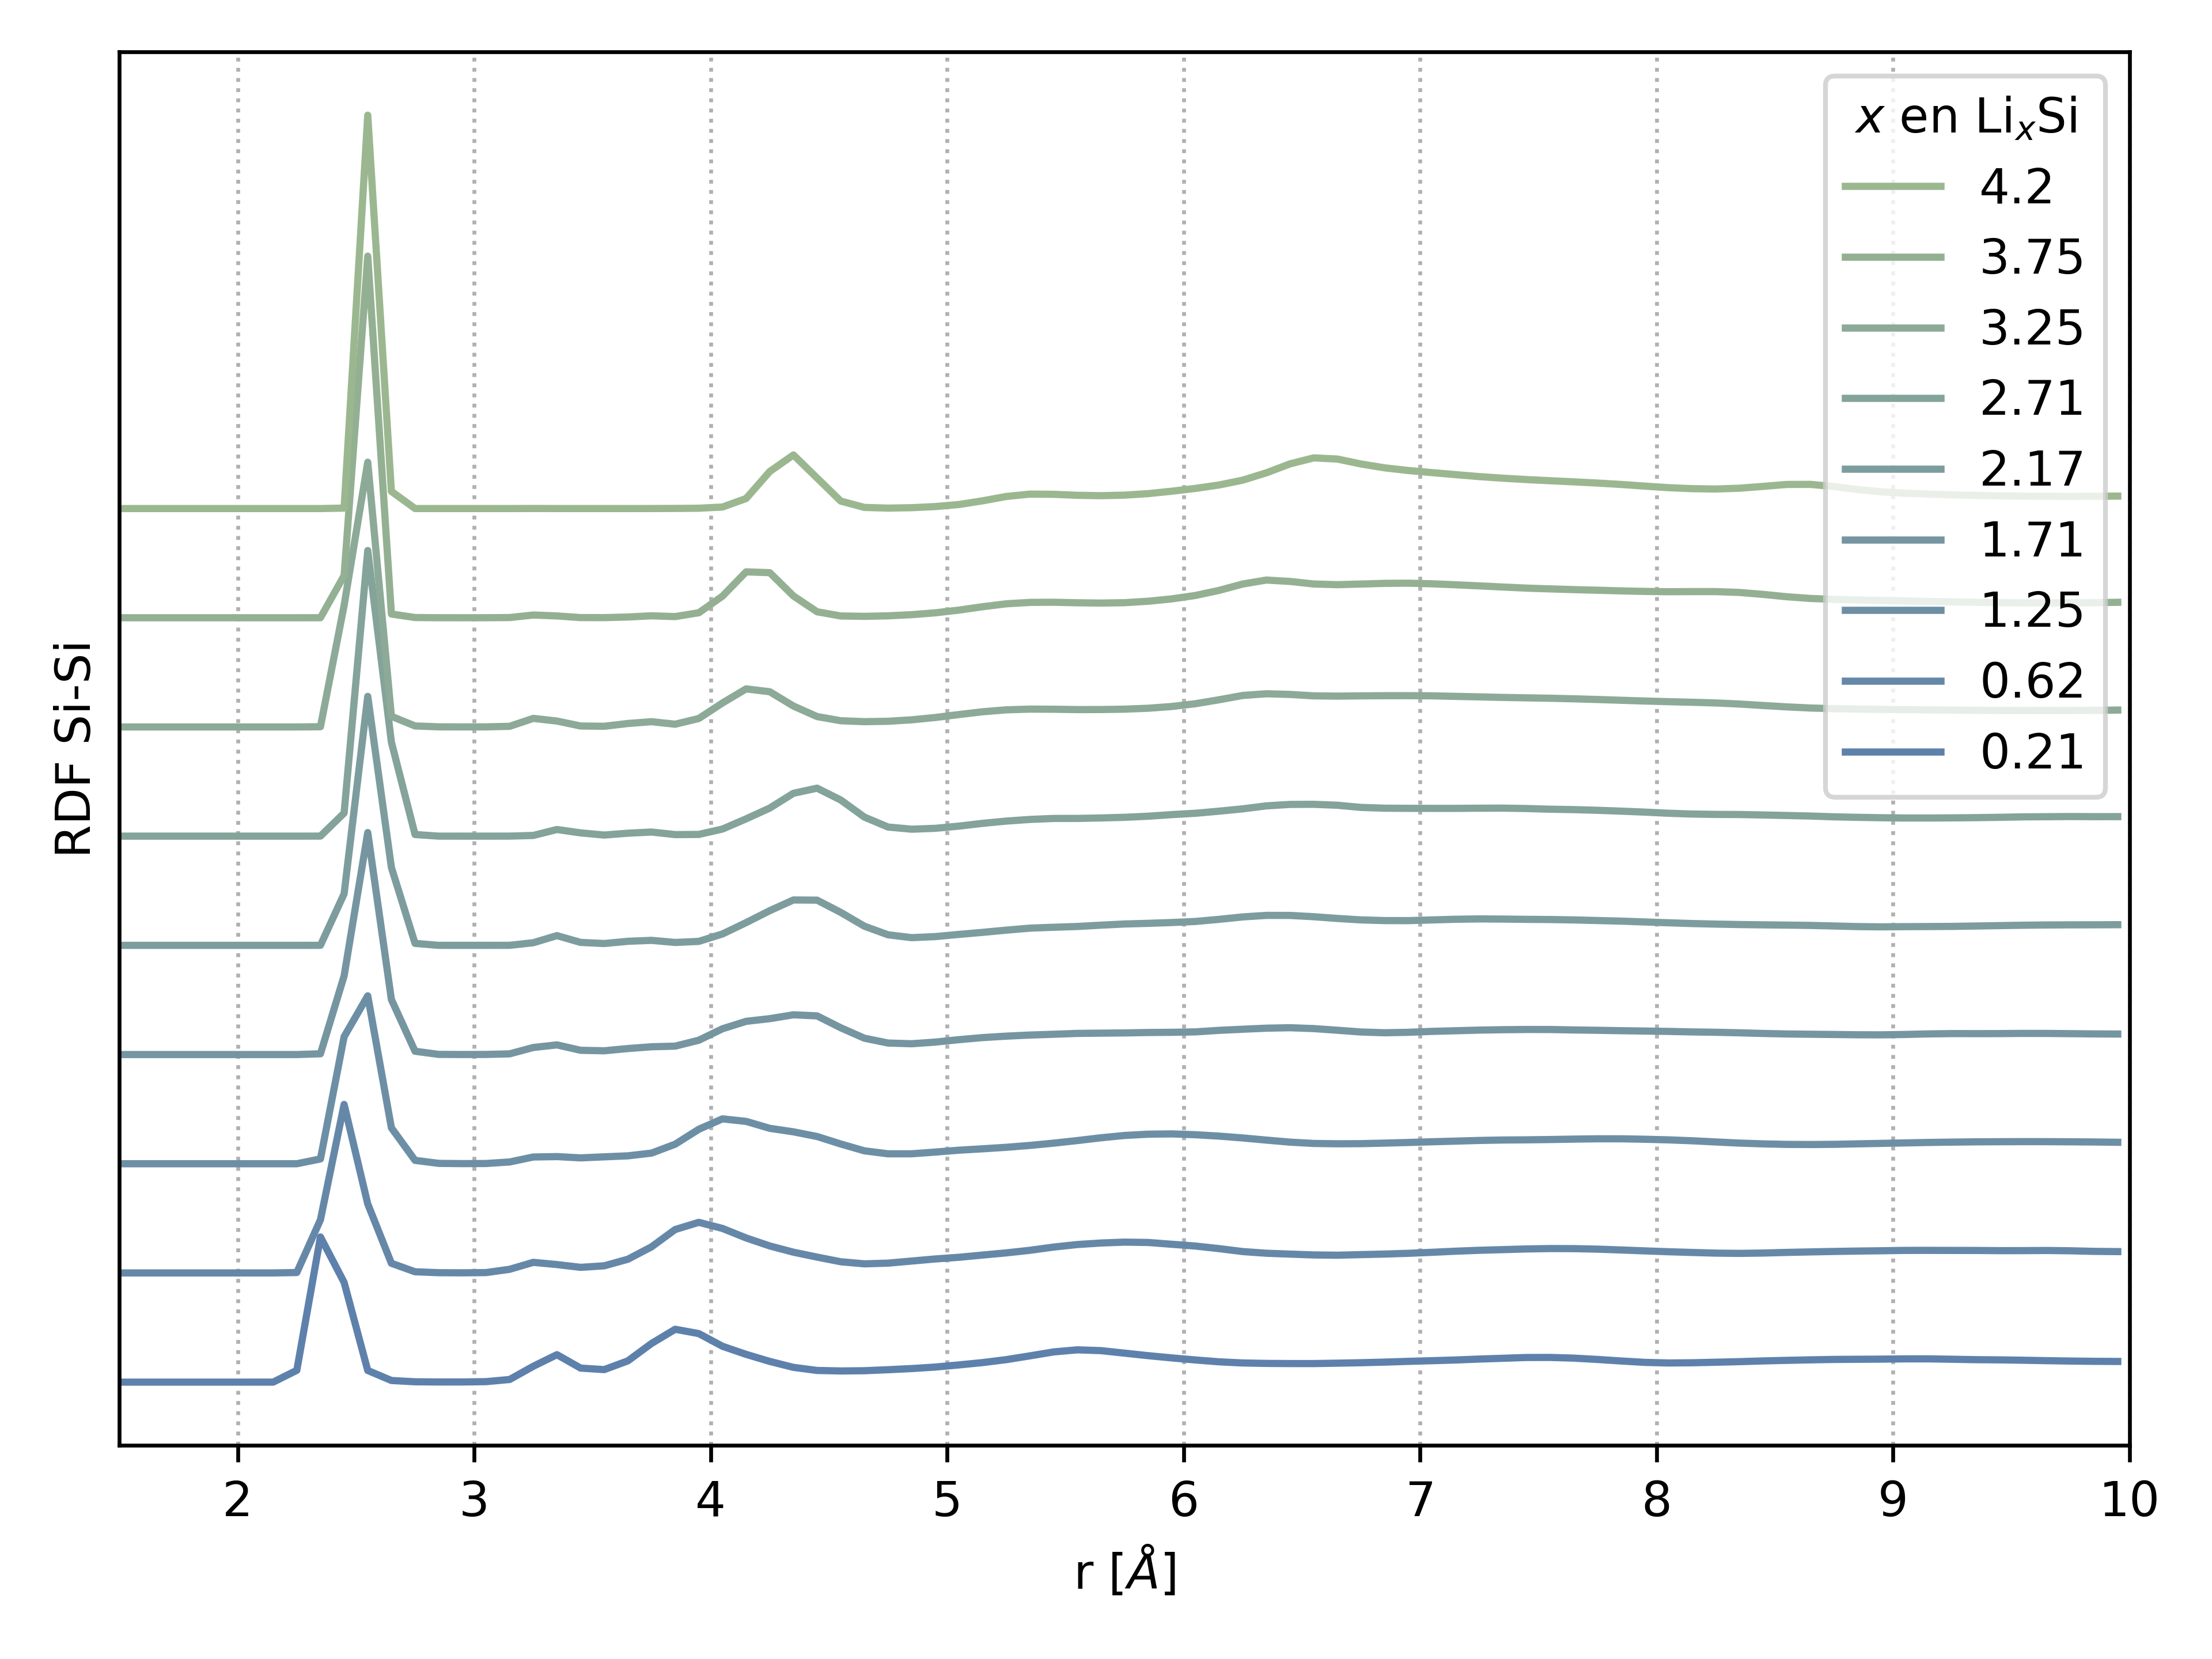
\includegraphics[width=0.8\textwidth]{caracterizacion/rdf-SiSi.png}
    \caption{Distribución radial de a pares para Si-Si de las estructuras 
    minimizadas. Cada curva se corresponde con un valor de concentración 
    distinto.}
    \label{fig:rdf-SiSi}
\end{figure}
Este mismo efecto se ve en el primer pico de la RDF$_{Si-Si}$, el centro del mismo
se encuentra en 2.4 \AA\ para $x = 0.21$ y luego se desplaza a distancias
mayores, después de $x = 1.25$ el centro se encuentra entre 2.52 y 2.56 \AA.
Mientras que la altura del pico aumenta se ve un decrecimiento en en el ancho 
del pico, el valor del FWHM va de 0.14 \AA\ a 0.05 \AA\ para $x = 0.21$ y 
$x = 3.75$, respectivamente. Por otro lado, el segundo pico de la RDF$_{Si-Si}$
también se desplaza hacia distancias mayores, se divide en dos picos para valores 
de $x$ entre 0.62 y 1.71 y vuelve a comportarse como un sólo pico para para 
concentraciones mayores. Entre el primer y el segundo pico se observa un hombro,
como señalaron previamente Fan \textit{et al.} ~\cite{fan2013}. Los resultados 
obtenidos para la RDF$_{Si-Si}$ están en concordancia con las mediciones 
experimentales reportadas por Key \textit{et al.} ~\cite{key2011}.

\begin{figure}[h!]
    \centering
    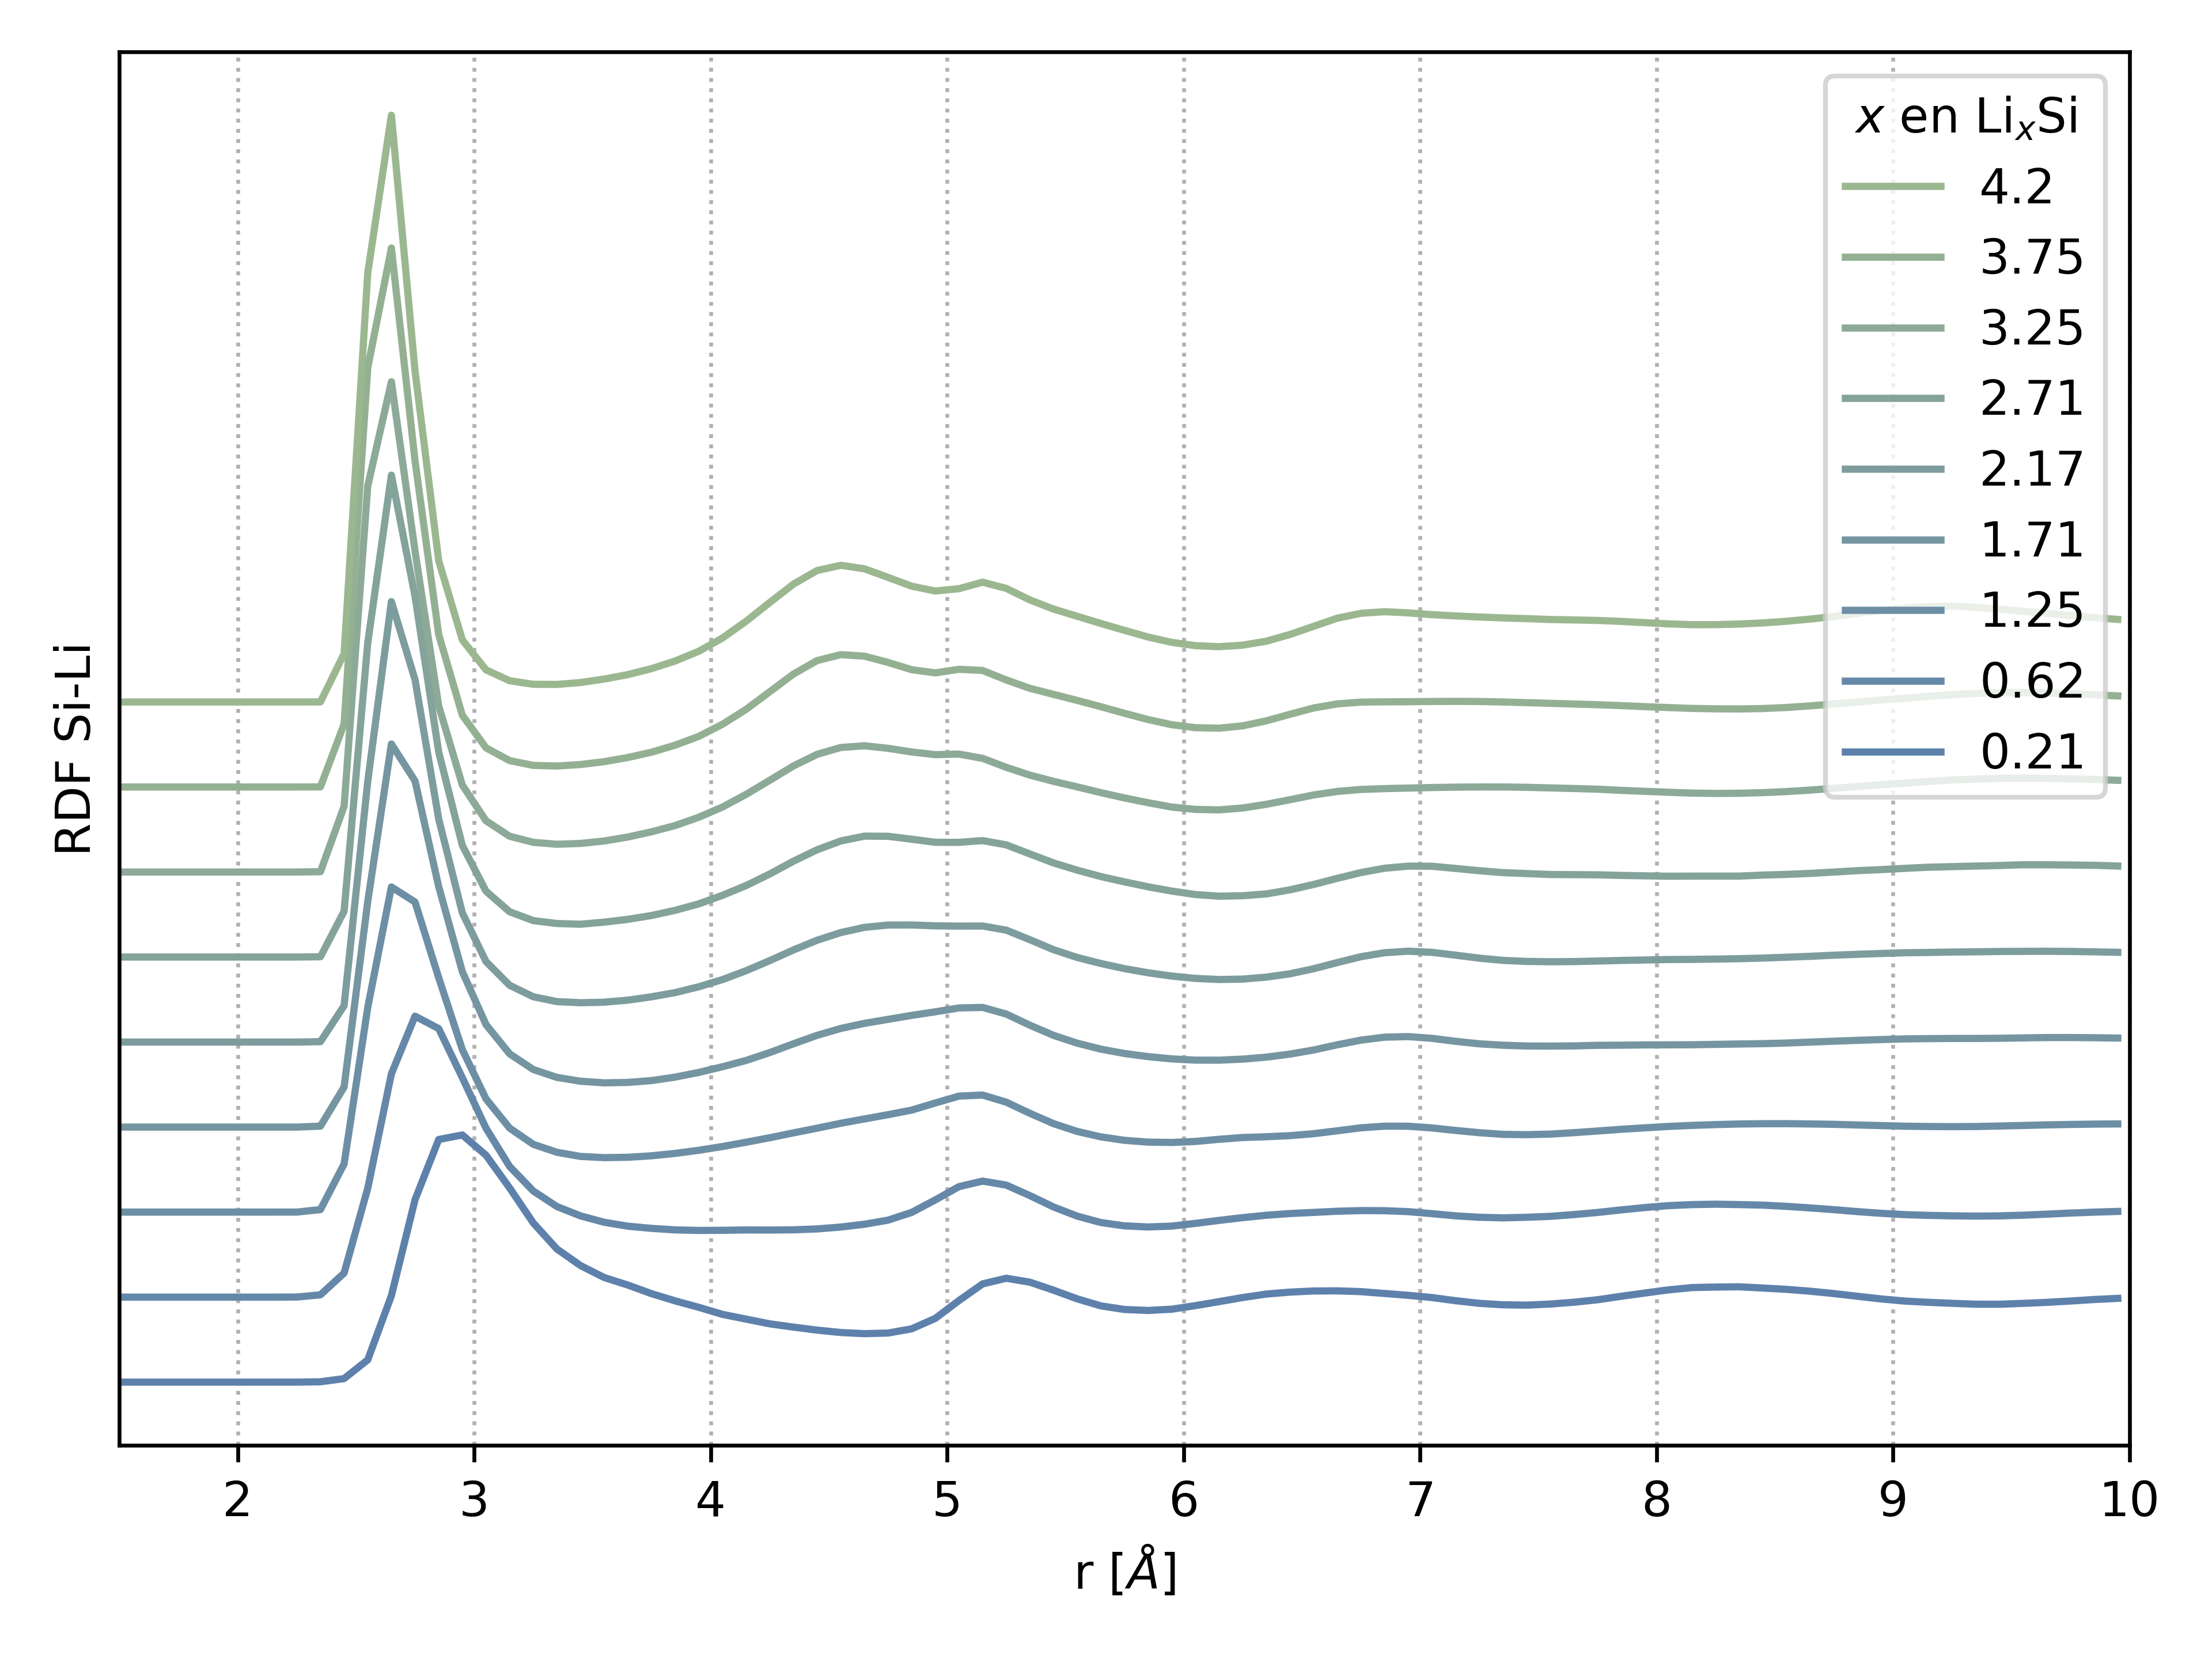
\includegraphics[width=0.8\textwidth]{caracterizacion/rdf-SiLi.png}
    \caption{Distribución radial de a pares para Si-Li de las estructuras 
    minimizadas. Cada curva se corresponde con un valor de concentración 
    distinto.}
    \label{fig:rdf-SiLi}
\end{figure}
Para el primer pico de la RDF$_{Si-Li}$ se ve el comportamiento contrario, el 
centro del mismo se desplaza a distancias menores a medida que la concentración
de litio aumenta. Esto es acompañado con un aumento de la altura del pico y una
disminución de su ancho. Para el segundo pico también se observa un desplazamiento
del mismo hacia distancias menores, pero por encima de $x = 1.71$ el pico se
divide en dos picos con distintas alturas dependiendo de la concentración. Esto
es analizado con mayor detalle en la sección \ref{s:intercionexion}.

\subsection{Número de coordinación}

De la misma manera que se definieron la distribuciones radiales de a pares parciales,
se pueden obtener los números de coordinación a un dado tipo de átomos. CN$_{ij}$
se corresponde con la cantidad de átomos vecinos de tipo $j$ para un átomo central
de tipo $i$ hasta una cierta distancia de corte. Para la elección de dicho valor 
se considera hasta el primer pico de la $g_{ij}(r)$ correspondiente. Debido a que 
en los materiales amorfos la primera y la segunda esfera de coordinación pueden 
llegar a estar superpuestas, el límite superior de integración no está definido 
unívocamente para todas las concentraciones consideradas ~\cite{lamparter1995}.
Para el número de coordinación promedio para átomos de Si vecinos de otros átomos 
de Si se calculó contando el número de dichos vecinos utilizando un radio de 
corte de 3 \AA. Lo mismo se realizó para Li-Li definiendo un radio de corte de 
4 \AA. Para el caso de Si-Li se utilizó el criterio de considerar como radio de 
corte el valor $r$ para el cual la $g(r)$ presenta un mínimo entre los dos picos
a primeros y segundo vecinos. Los resultados se muestran en la figura 
\ref{fig:cn1}.
\begin{figure}[th]
    \centering
    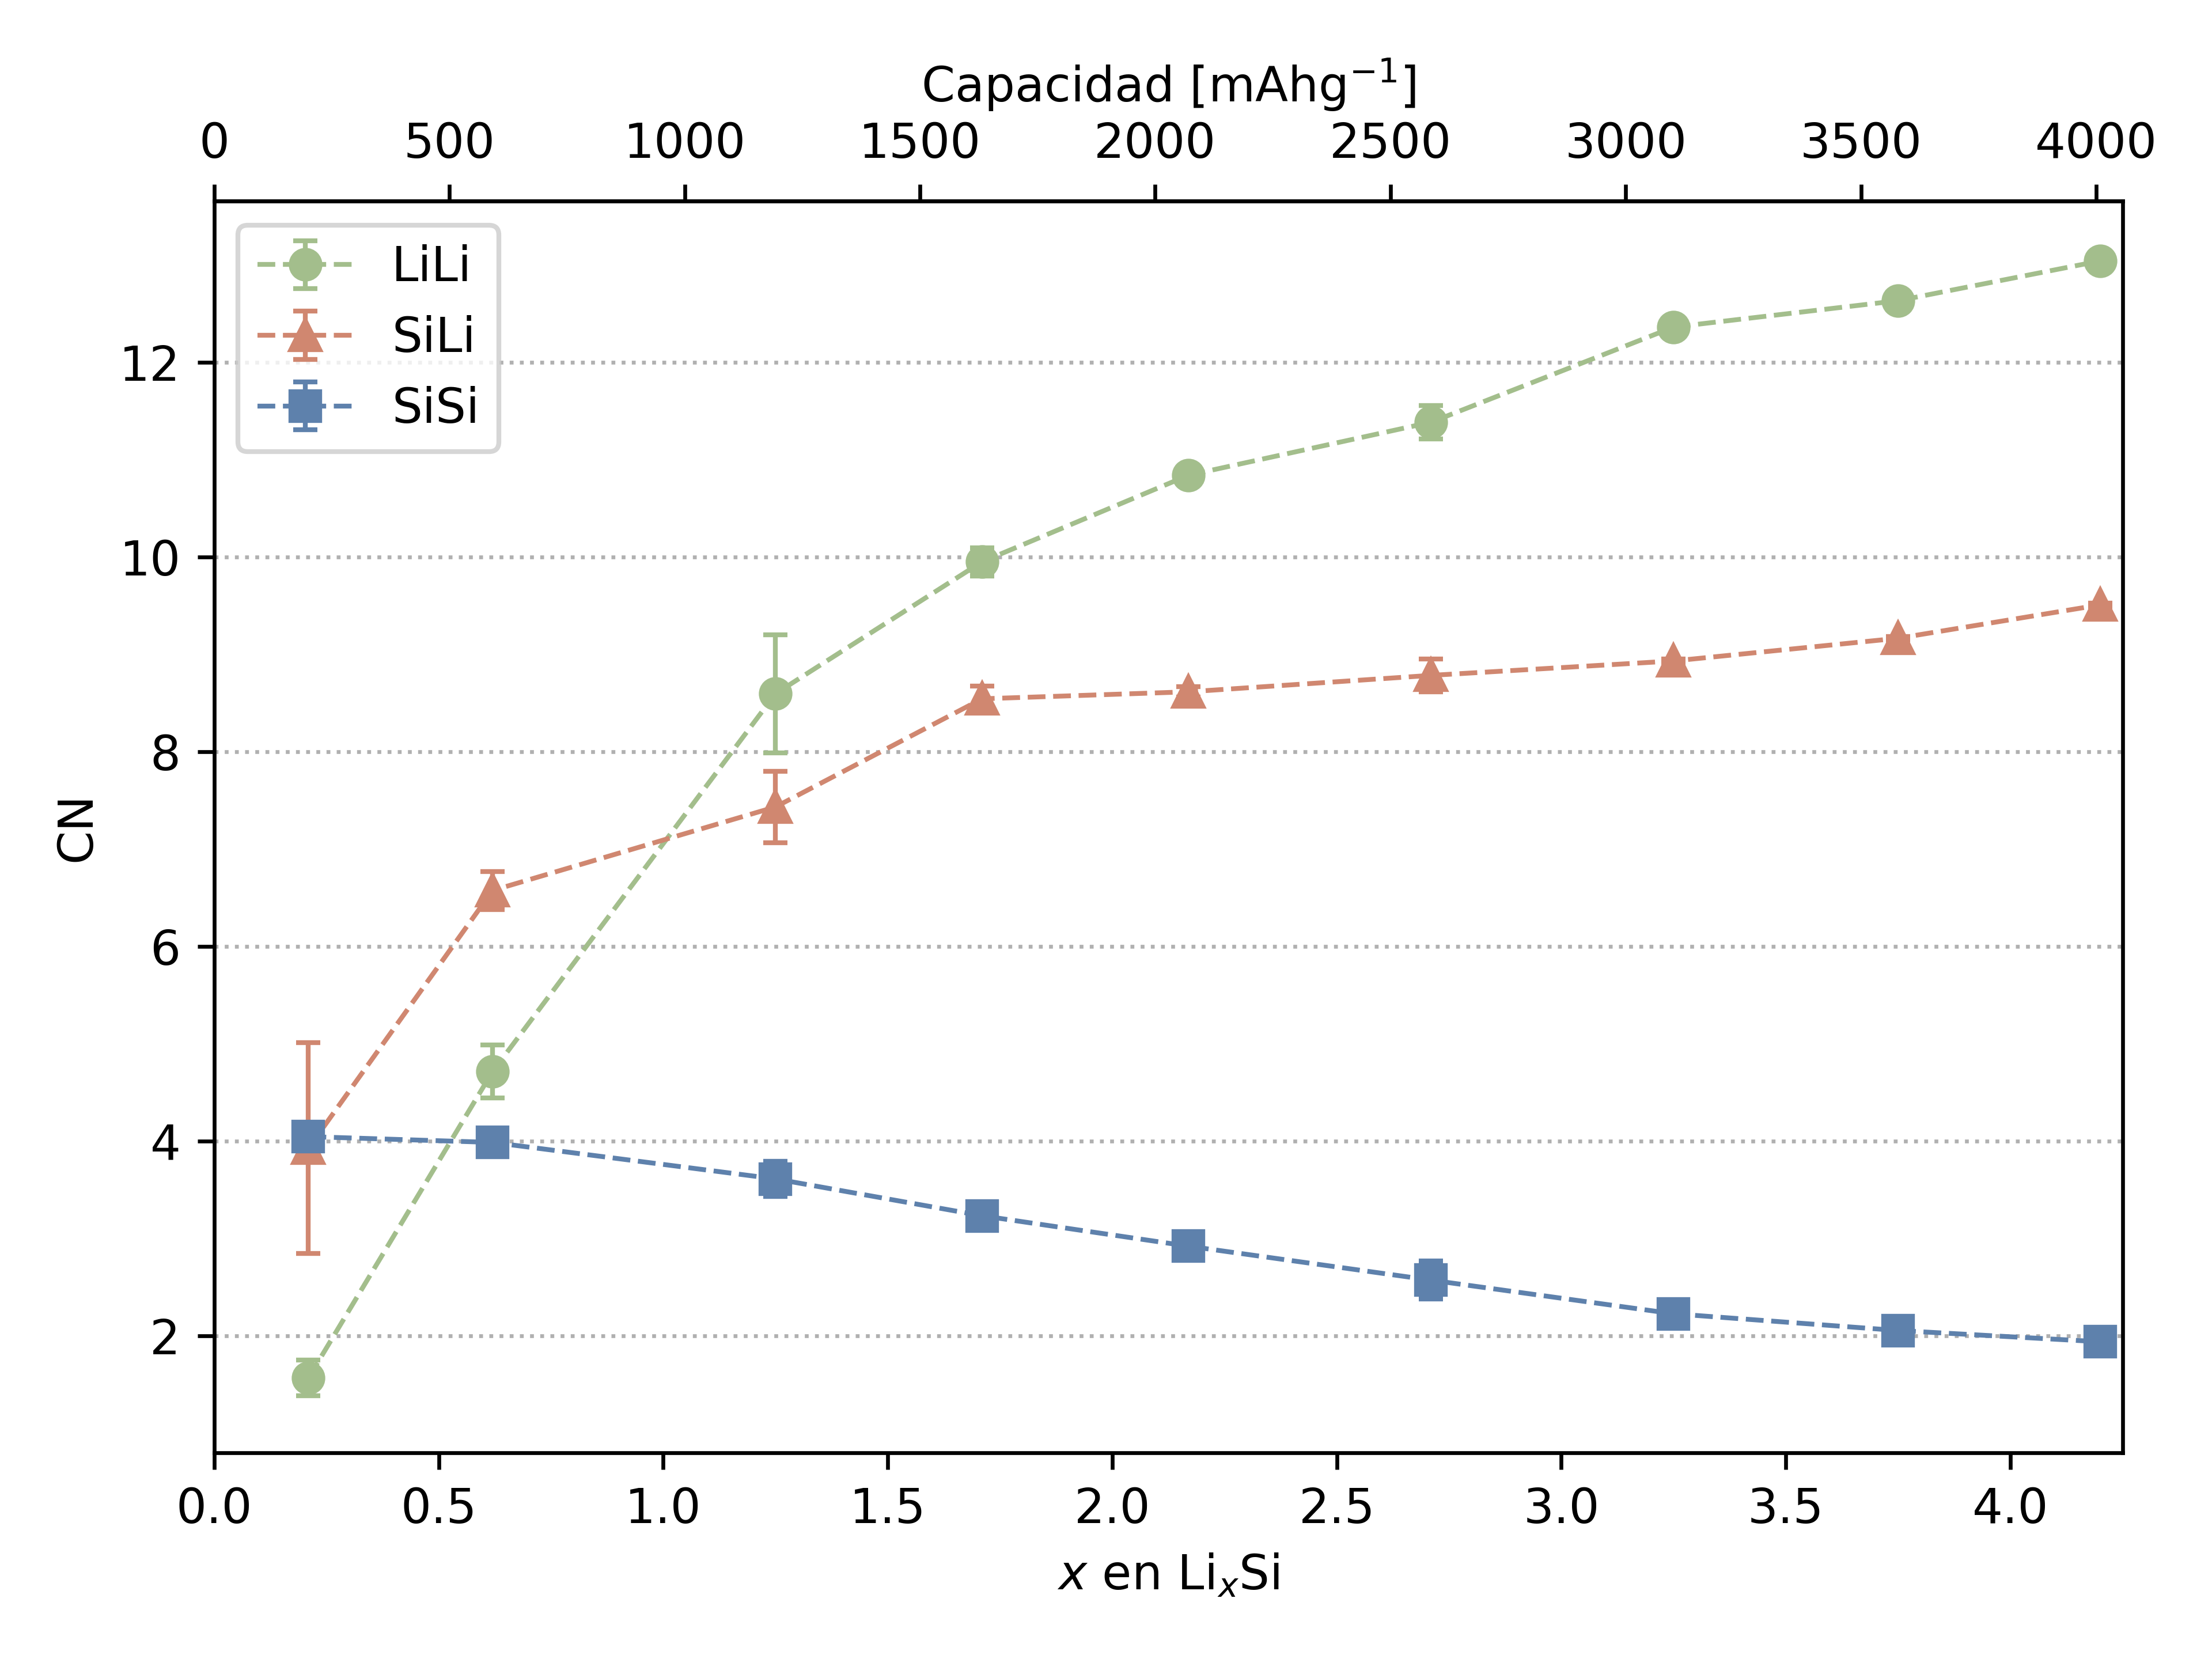
\includegraphics[width=0.8\textwidth]{caracterizacion/cn.png}
    \caption{Promedio del primer número de coordinación en función de la 
    concentración de litio para Li-Li, Si-Si y Si-Li. Como radio de corte se 
    utilizó la distancia posterior al primer pico de la RDF correspondiente. En 
    los casos en que no se aprecia la barra de error, es porque la misma es menor 
    que el tamaño de los puntos.}
    \label{fig:cn1}
\end{figure}

Para el caso del CN$_{Si-Si}$, se tiene que esta cantidad decrece de 4 a 2, a 
medida que la concentración de Li aumenta. Esto indica que a valores pequeños de 
$x$ la estructura de Si mantiene sus conexiones tetraédricas, mientras que para
valores grandes de $x$ el Si tiende a formar cadenas periódicas unidimensionales.
En la red de silicio amorfa, analizada con más detalle en la sección 
\ref{s:clusters}, una estructura 3-periódica se presenta para valores bajos de 
$x$, donde el CN se encuentra alrededor de 4. Luego, se alcanza una estructura 1-periódica 
para valores grandes de $x$, donde los enlaces Si-Si tienden a formar 
cadenas, que pueden verse para $x = 3.75$ donde se tiene $CN = 2.05$, por ejemplo.
El CN de Si-Li y Li-Li presenta valores pequeños para concentraciones 
bajas y aumenta monótonamente hasta alcanzar valores de 10 y 12, respectivamente, 
que se asemejan al valor de una estructura de empaquetamiento compacto.

\begin{figure}[th]
    \centering
    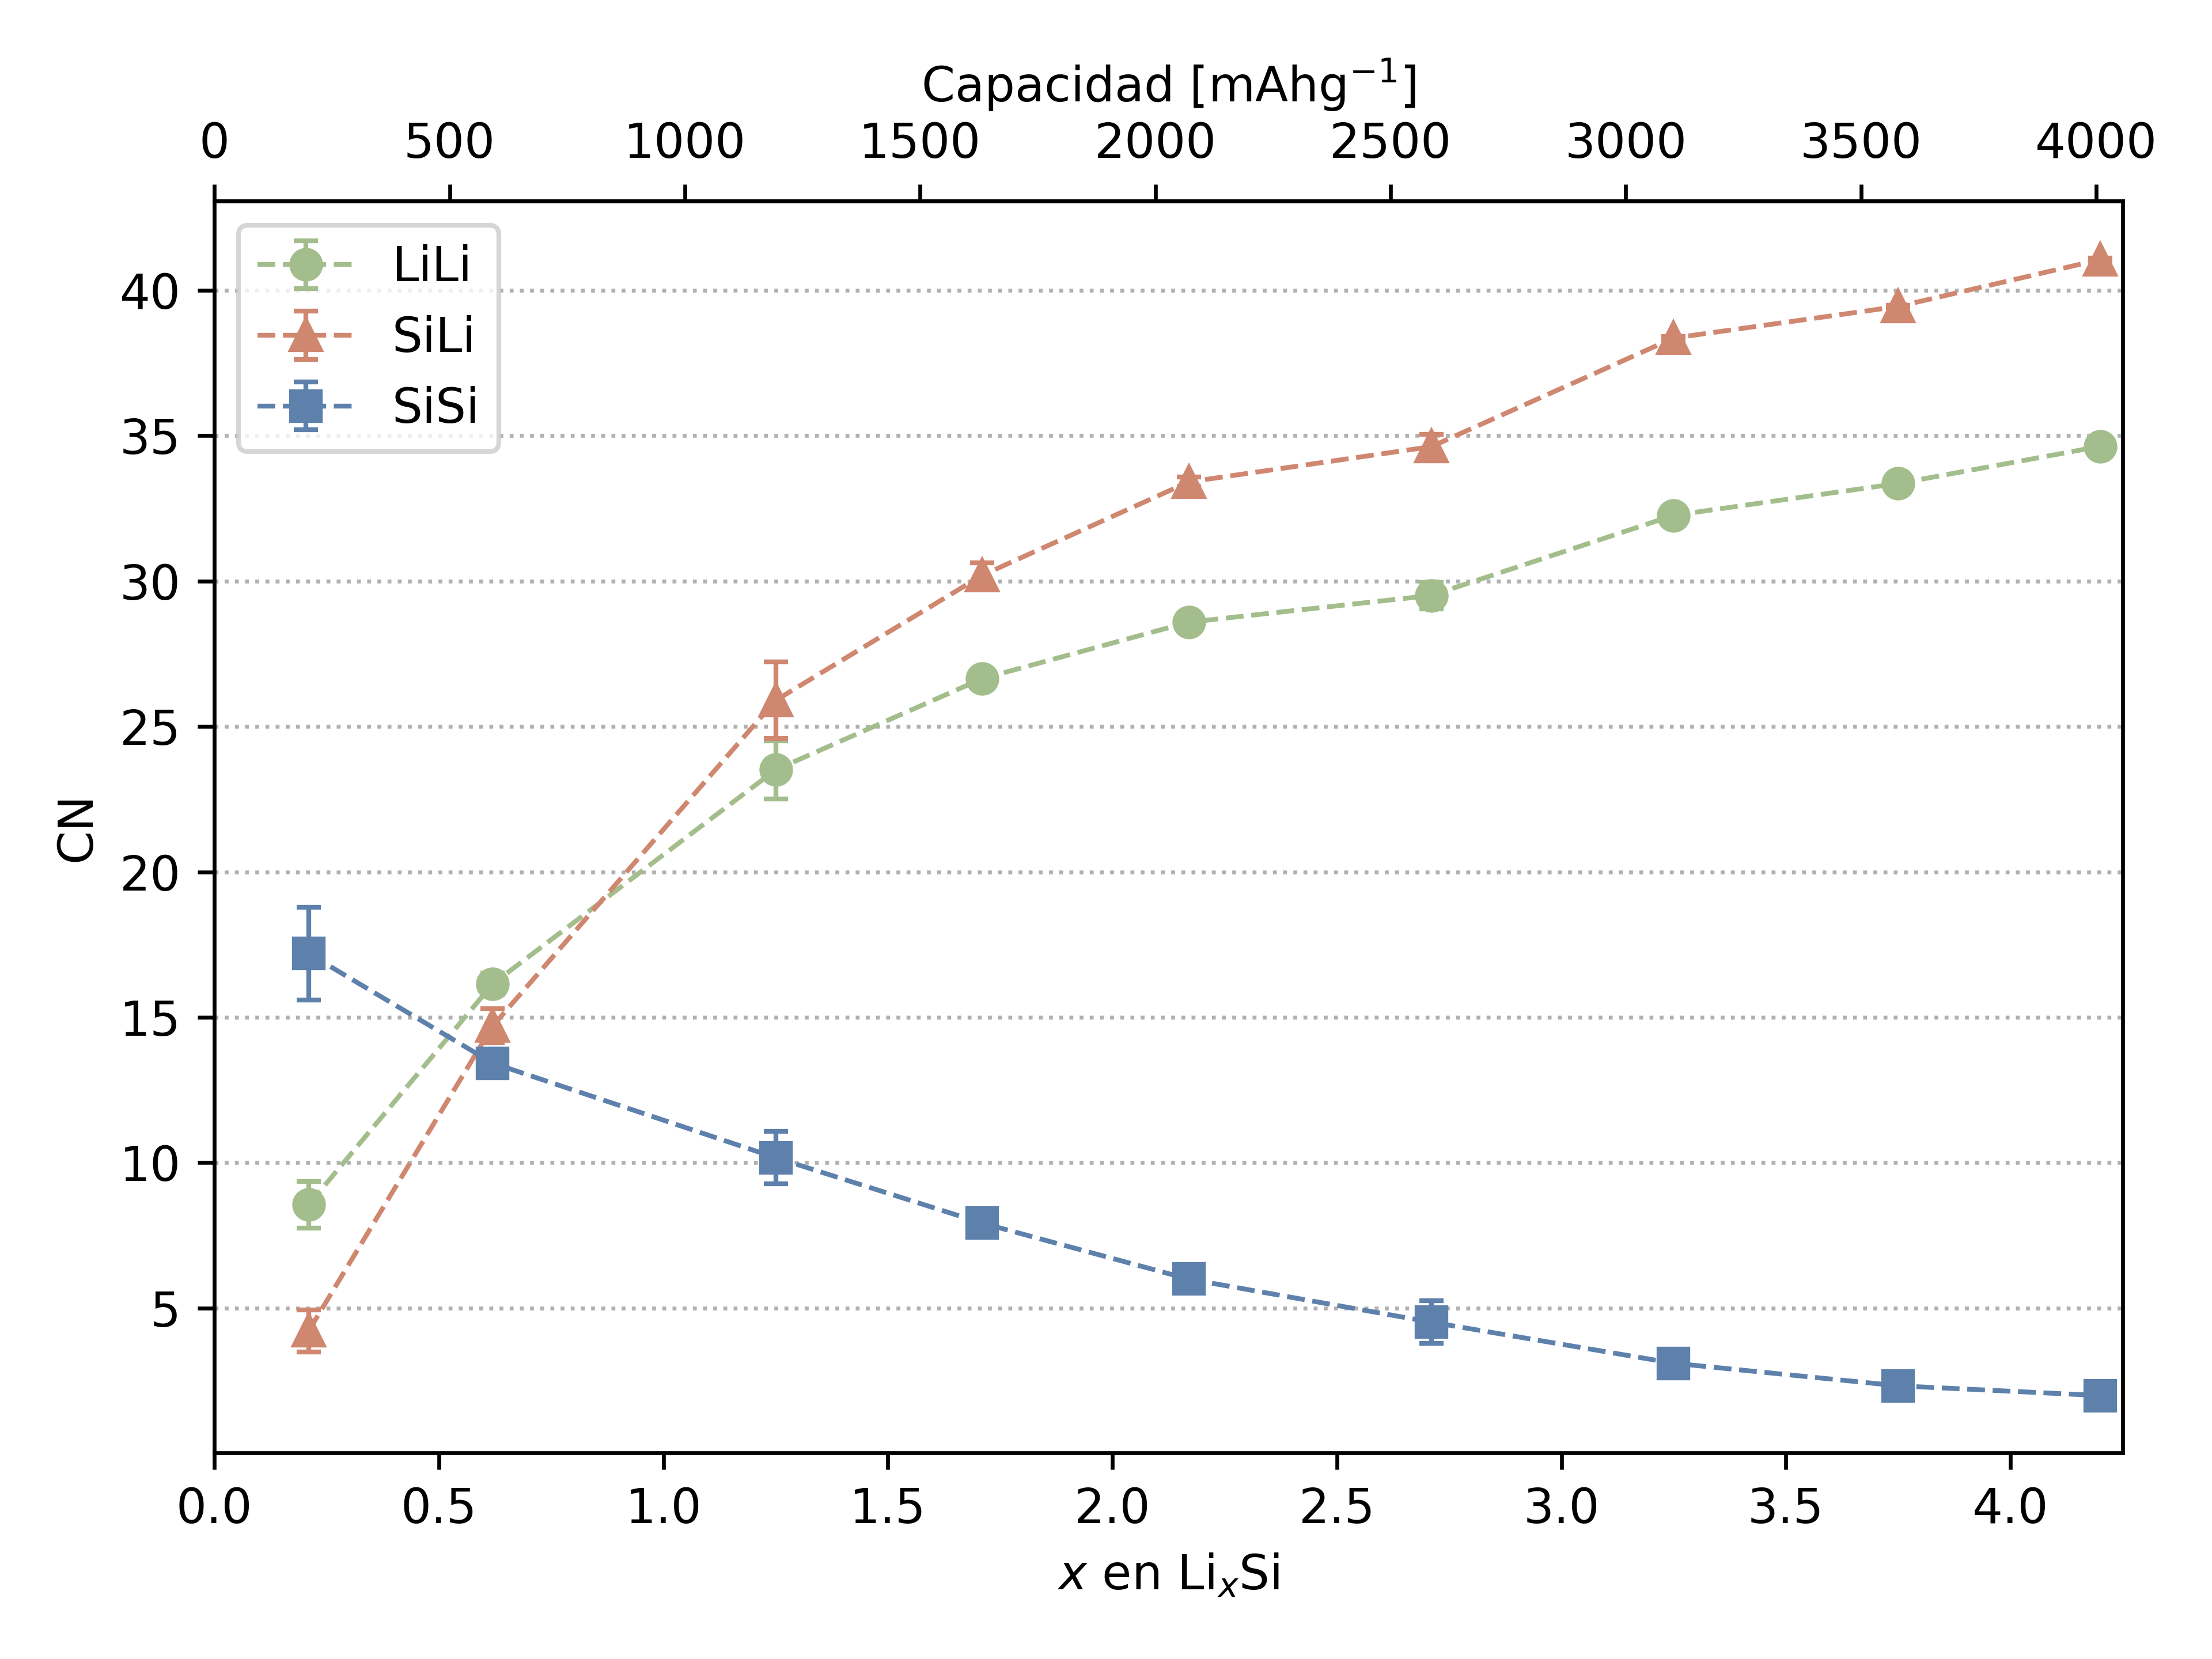
\includegraphics[width=0.8\textwidth]{caracterizacion/cn2.png}
    \caption{Promedio del segundo número de coordinación en función de la 
    concentración de litio para Li-Li, Si-Si y Si-Li. Para la elección de los 
    radios de corte que definen el cascarón en el cual se cuentan los vecinos,
    se consideró el segundo pico de la RDF correspondiente. En los casos que no 
    se aprecia la barra de error, es porque la misma es menor que el tamaño de 
    los puntos.}
    \label{fig:cn2}
\end{figure}
Los resultados para el segundo número de coordinación se presentan en la figura 
\ref{fig:cn2}. Estos resultados se obtuvieron considerando un cascarón con un 
radio de corte interno y otro externo, elegidos de manera tal que incluyan el 
segundo pico de la RDF. La elección de dichos valores varió dependiendo del tipo
de átomos que se consideraron. En todos ellos se tomó como radio de corte interno 
el radio de corte del primero número de coordinación. Luego, para el radio de 
corte externo se utilizaron valores de 5.0 \AA\ para Si-Si y 6.0 \AA\ para Li-Li
y Si-Li.

Para los valores de CN$_{Si-Si}$ se observa un aumento para concentraciones bajas
de Li si se lo compara con el CN de primeros vecinos. Para valores mayores de $x$,
se puede ver como el valor de CN también tiende a 2, lo cual es coherente con la
formación de cadenas que se notó previamente. La tendencia cualitativa del segundo
CN para Li-Li y Si-Li es la misma a la observada en el primer CN, sólo que ahora
empieza en un valor cercano a 5 y tiende a 35 y 40, respectivamente. Este valor 
es mucho mayor que el que se tiene para los segundos vecinos en una estructura 
de empaquetamiento compacto, que es 6 para la estructura cristalina FCC. Incluso 
es mayor a la suma del segundo (6) y del tercer vecino (24) esperado para la red 
FCC.

\subsection{Formación de conglomerados (clusters)}\label{s:clusters}

Analizando la formación de conglomerados (clusters) por medio del algoritmo DBSCAN 
~\cite{ester1996}, en el cual puede definirse un radio de corte para el cual se 
deja de considerar que los átomos están enlazados entre sí (es decir, formando 
clusters), se encuentra que las estructuras amorfas de silicio no pueden ser 
clasificadas en diferentes tipos de clusters, las mismas reflejan más bien 
una red amorfa. Esto viene de interpretar los gráficos que se presentan en la 
figura \ref{fig:clusters}. 

En particular, en la figura \ref{fig:clusters-isolated} se define el porcentaje 
de átomos de Si que están a una distancia mayor que $r_{cut}$ de otros átomos de 
Si, cuando el radio de corte es mayor que la distancia a la cual termina el 
primer pico de la RDF$_{Si-Si}$, no se tienen átomos de Si que cumplan esta 
propiedad, es decir, no hay átomos de Si que se encuentren aislados en el sistema,
incluso a concentraciones altas de Li. Esto refleja que el a-Si se comporta como 
una red en la cual todos los átomos de silicio están interconectados entre sí, 
cosa que también se puede deducir de la figura \ref{fig:clusters-nclusters}, en la cual 
se tiene que cuando el radio de corte es menor que el primer pico de la RDF$_{Si-Si}$ 
el número de clusters es igual al número de átomos de Si, pero que cuando este 
radio es más grande que la distancia a la cual termina el primer pico, hay un 
solo cluster.

\begin{figure}[h]
    \centering
    \begin{subfigure}{.475\textwidth}
        \centering
        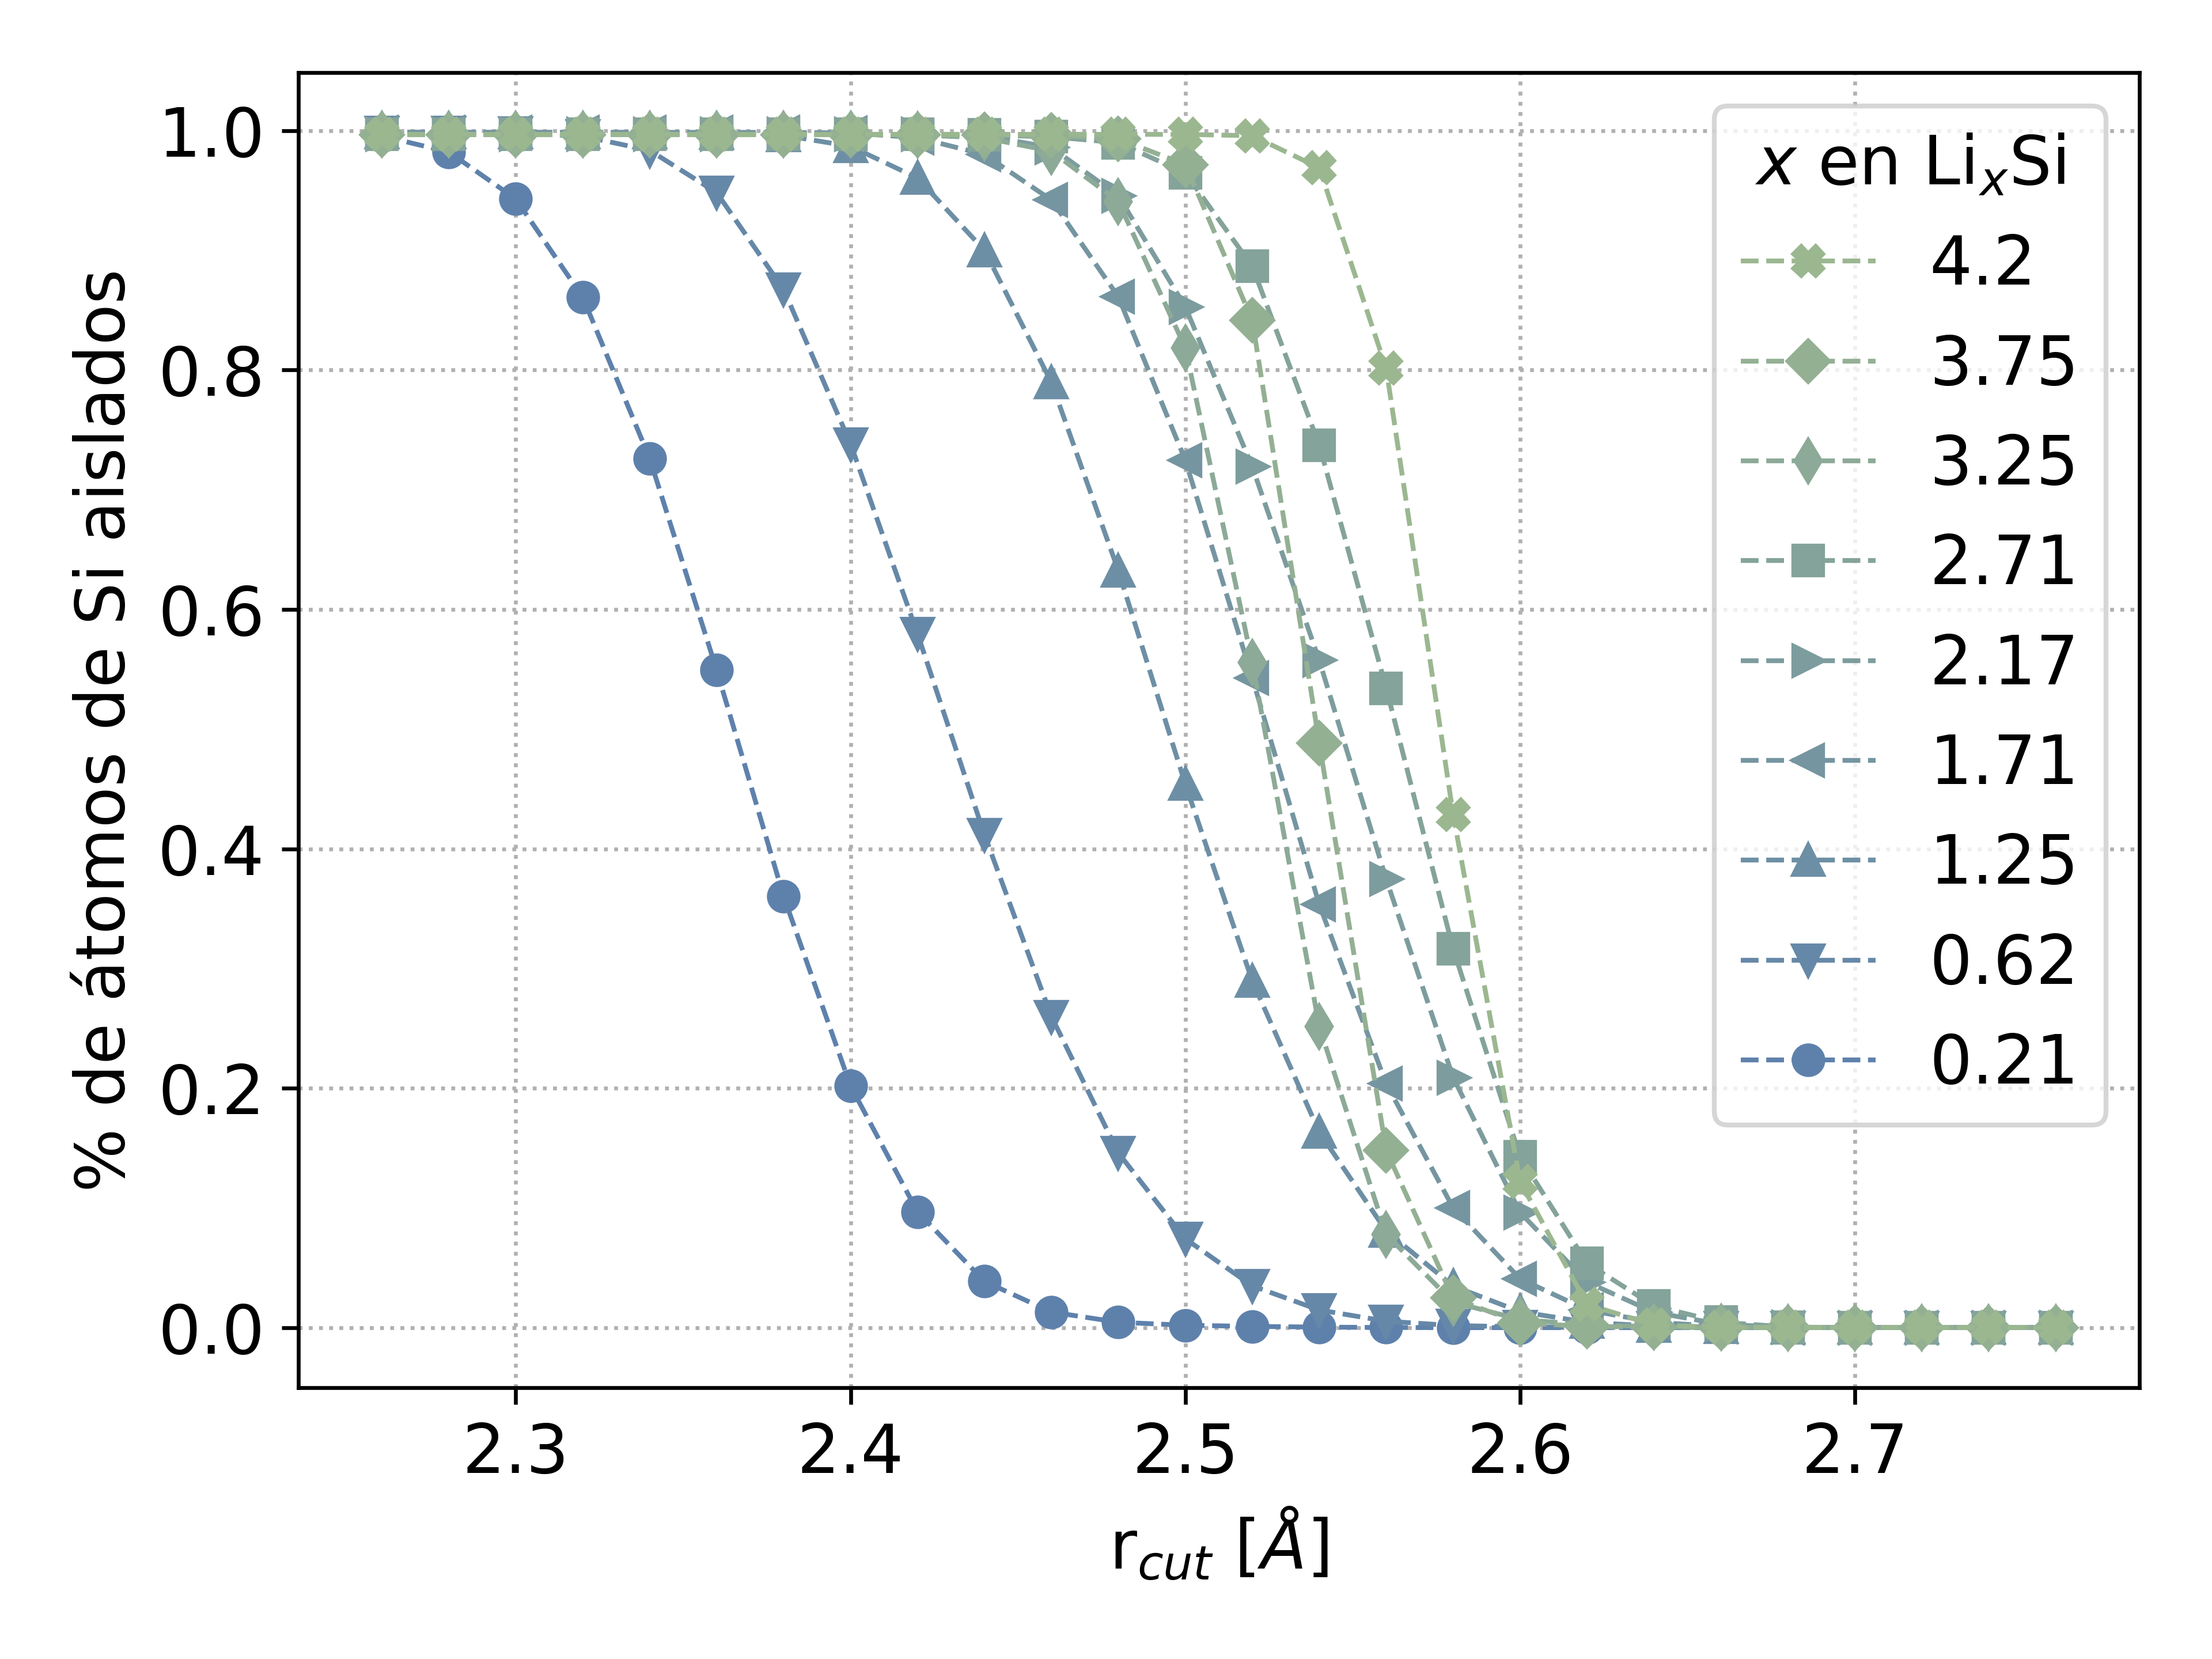
\includegraphics[width=\textwidth]{caracterizacion/cluster-isolated.png}
        \caption{Porcentaje de átomos de Si aislados en función de la elección del
        radio de corte.}
        \label{fig:clusters-isolated}
    \end{subfigure}
    \hfill
    \begin{subfigure}{.475\textwidth}
        \centering
        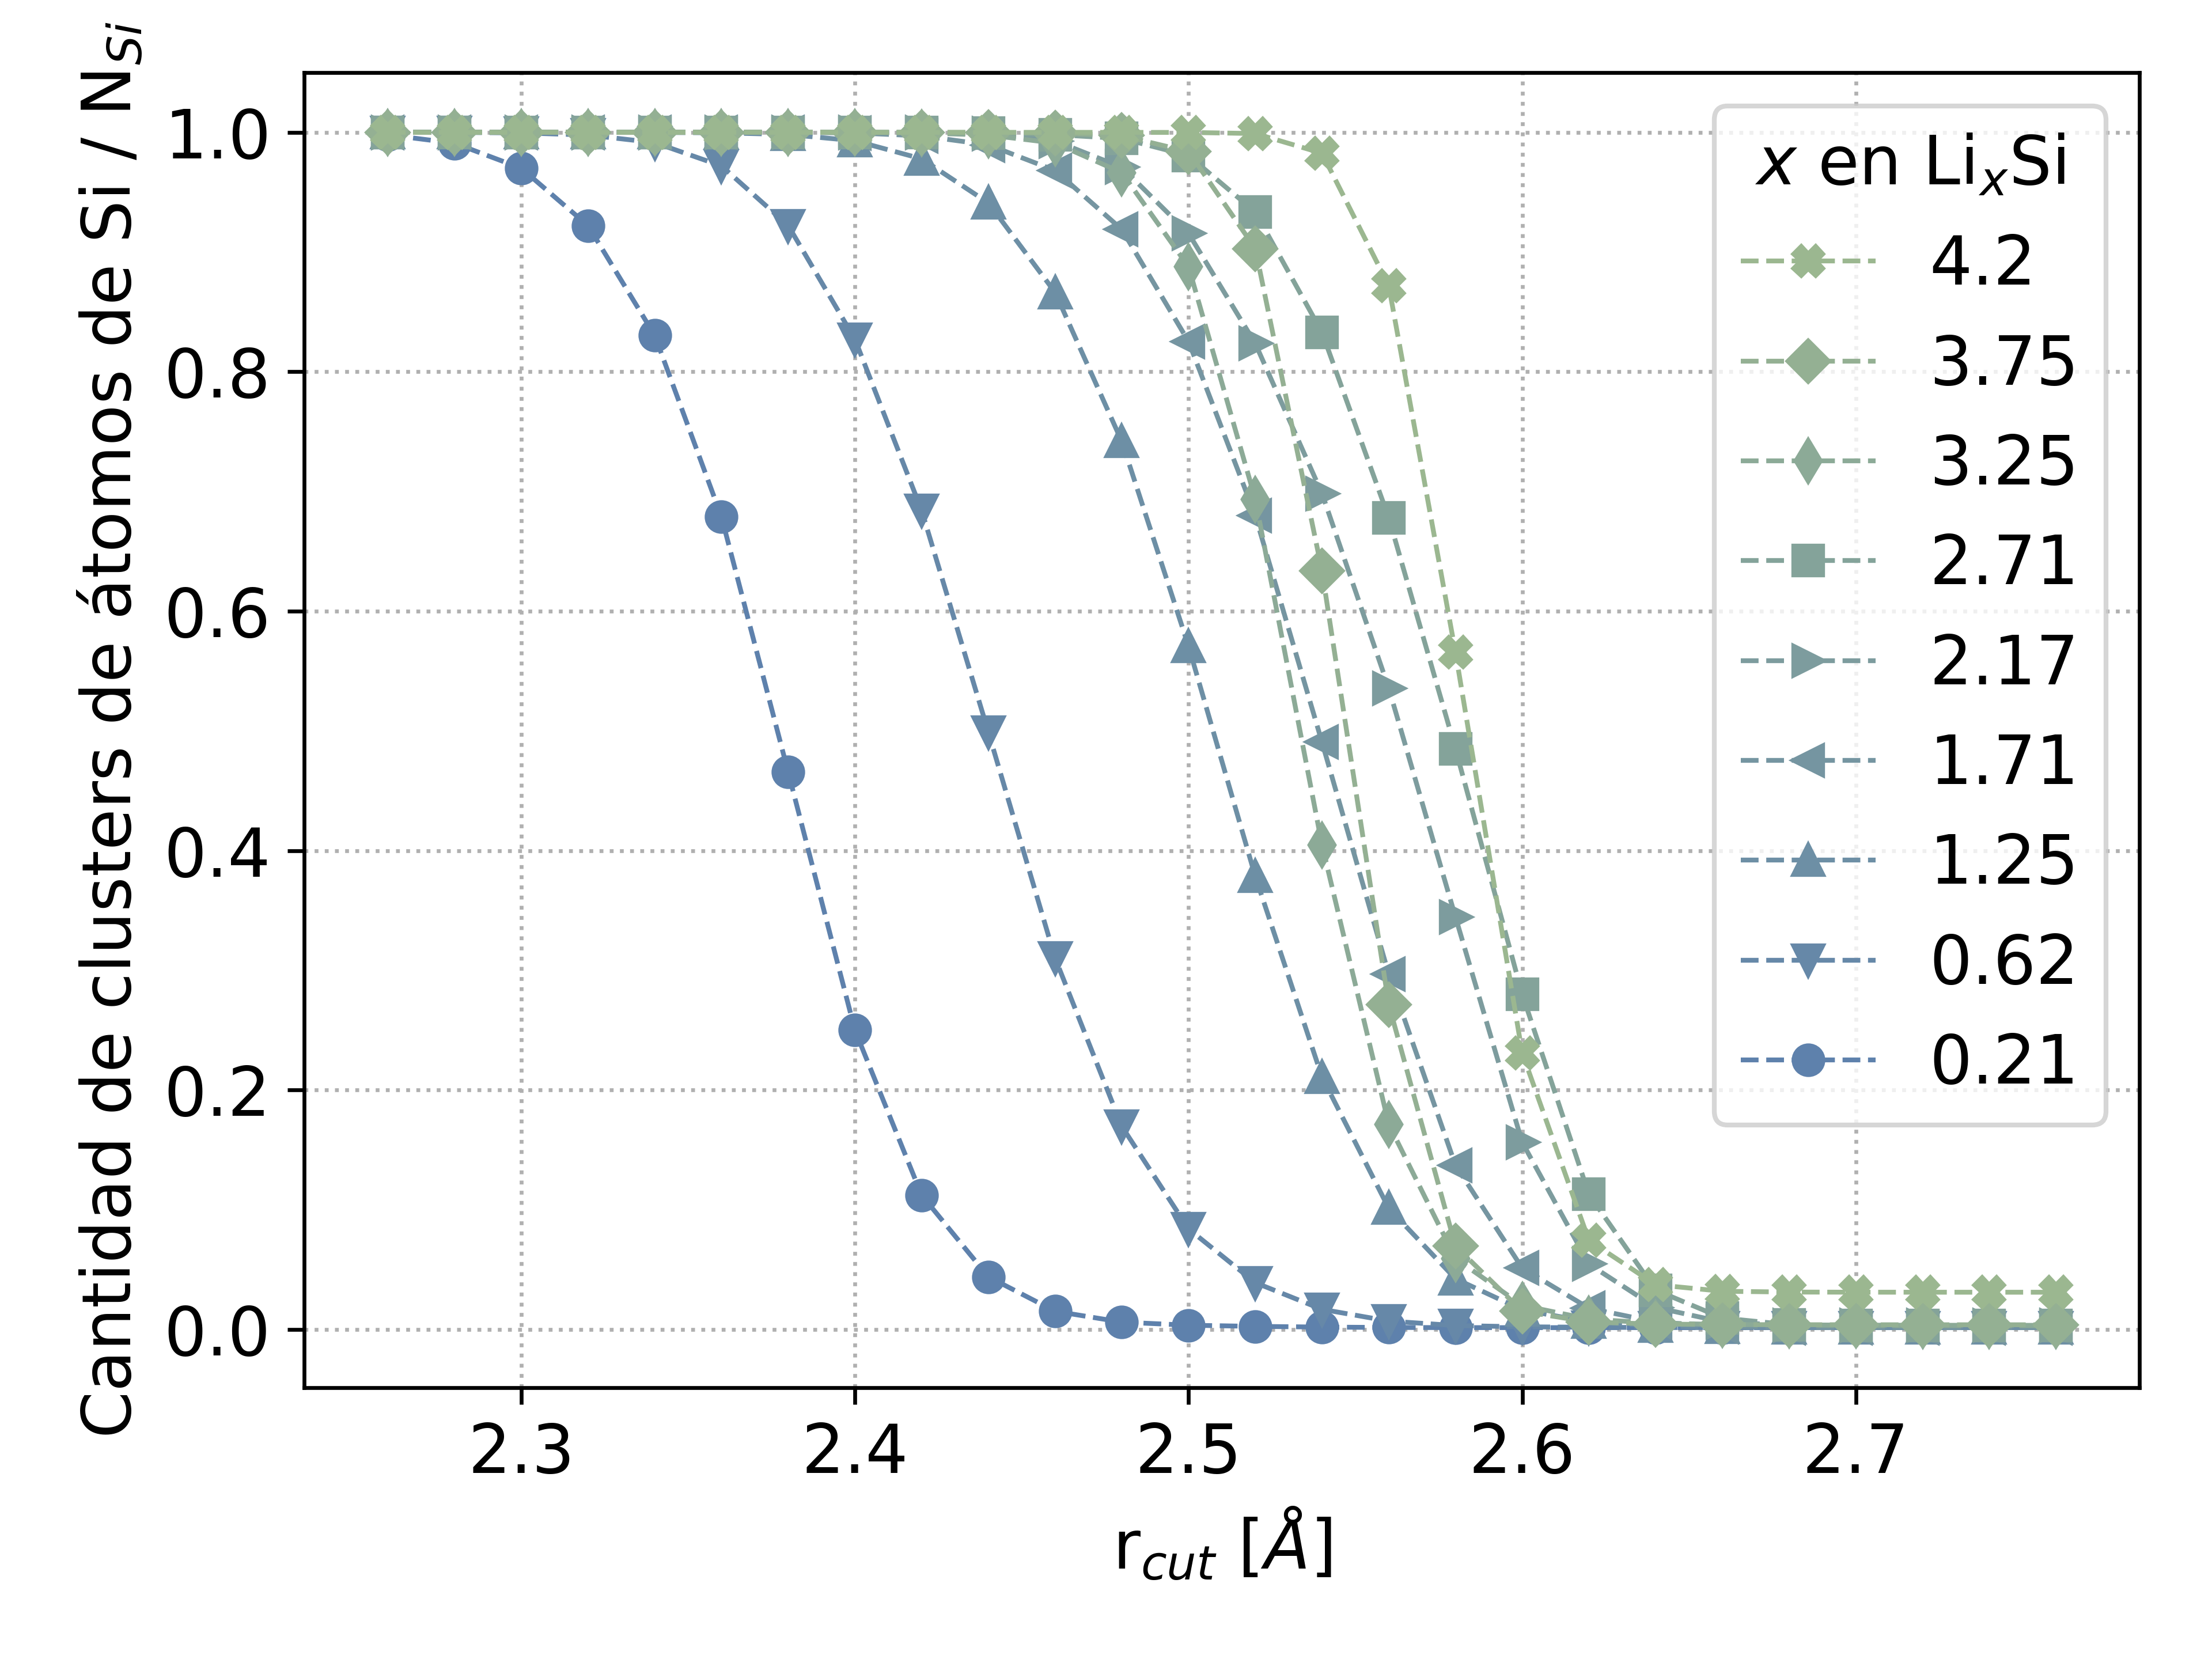
\includegraphics[width=\textwidth]{caracterizacion/cluster-nclusters.png}
        \caption{Número de clusters de Si sobre el número total de átomos de Si.}
        \label{fig:clusters-nclusters}
    \end{subfigure}
    \caption{Formación de clusters indicando una red amorfa de silicio.}
    \label{fig:clusters}
\end{figure}

\subsection{Interconexión de clusters}\label{s:intercionexion}

Para determinar qué es lo que causa la división en el segundo pico de la 
RDF$_{Si-Li}$ se realizó un análisis similar al reportado por Ding \textit{et al.}
~\cite{ding2015}. Estos autores analizaron la correlación en la distancia de a
pares de los segundos vecinos más cercanos en términos de las conexiones entre
clusters, definiendo un poliedro de coordinación alrededor del átomo central 
considerado para la RDF y sus segundos vecinos. El número de átomos compartidos
entre estos dos poliedros de coordinación enlazados fueron utilizados para 
establecer categorías y analizar sus contribuciones a la RDF. Estas categorías
dependen del hecho de que los poliedros comparten un vértice (1 átomo), una 
arista (2 átomos), una cara de los poliedros (3 átomos) o cuadriláteros 
distorsionados o tetraedros aplastados (4 átomos). De una forma similar a este 
trabajo, se deconvolucionó el segundo pico de la RDF calculando la RDF parcial 
de distintas categorías, donde cada categoría se define por el número de átomos de
Li que interconectan un átomo de Si con su segundo vecino de Li. El comportamiento
detallado se presenta en la figura \ref{fig:interconexiones}. Puede afirmarse a 
grandes rasgos que para concentraciones bajas de Li en las aleaciones, hay una 
predominancia de segundos vecinos de Li que tienen una o ninguna interconexión 
con los vecinos de Li de la primera esfera de coordinación Si-Li. Para $x > 1.0$
la contribución del segundo vecino de Li interconectado con dos o más átomos de 
Li de la primera esfera de coordinación Si-Li comienza a ser predominante y la
contribución de los átomos de Li sin conectarse empieza a decaer. Para $x > 3.0$,
la contribución del primer pico del segundo vecino de Li interconectado dos o
tres veces se vuelve relevante mientras que aparecen contribuciones de cuatro o
más interconexiones.
\begin{figure}[th]
    \centering
    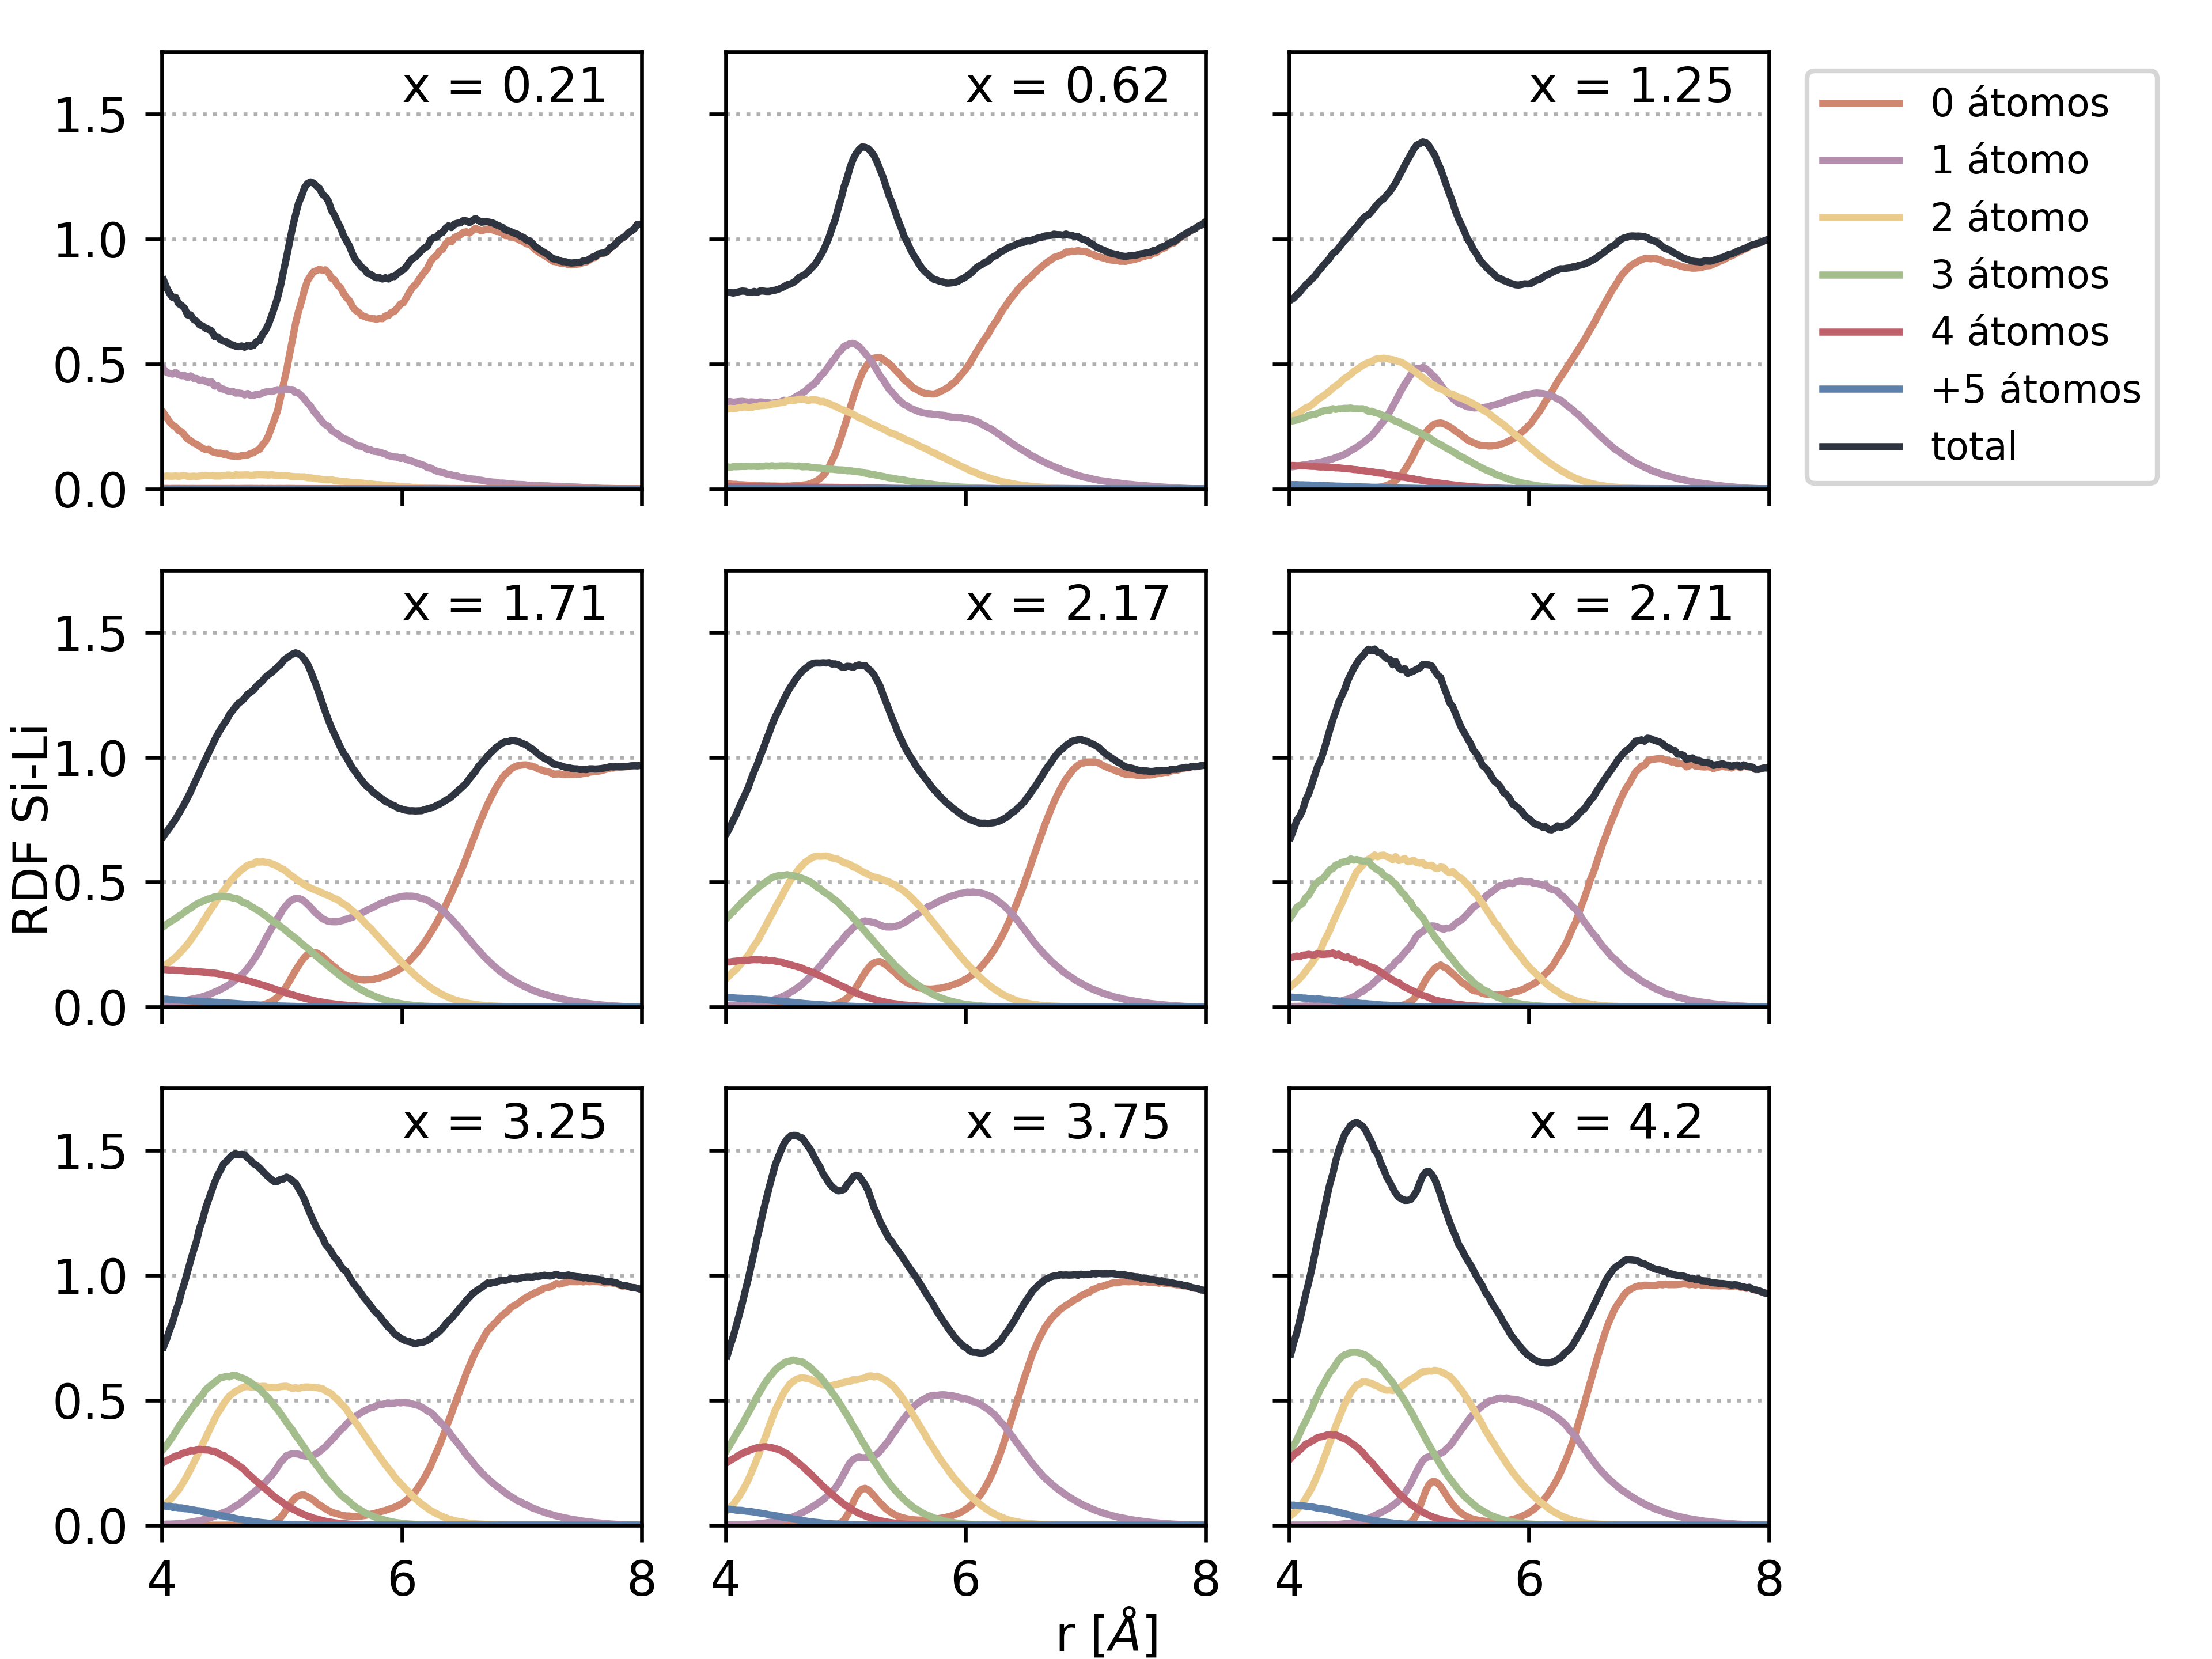
\includegraphics[width=\textwidth]{caracterizacion/interconexiones.png}
    \caption{Interconexiones de los segundos vecinos más cercanos de Li con un 
    átomo central de Si para cada valor de $x$ en Li$_x$Si considerado. El número 
    de primeros vecinos más cercanos que conectan a los segundos vecinos más 
    cercanos con el átomo central de Si se indica en el recuadro de las figuras. 
    Además de la RDF$_{Si-Li}$ total, se grafica cada una de las contribuciones 
    de los diferentes tipos de interconexiones posibles.}
    \label{fig:interconexiones}
\end{figure}

Mientras que el comportamiento presentado en la figura \ref{fig:interconexiones}
es más bien complejo, pueden establecerse tendencias generales que ayudan a 
entender mejor que es lo que sucede. Si se divide la RDF$_{Si-Li}$ en dos 
contribuciones de segundos vecinos, la primera de ellas, que se encuentra a una
distancia entre 4.0 \AA\ y 5.0 \AA, se puede atribuir a los átomos que tienen dos 
o más interconexiones de Li, mientras que la segunda de ellas, entre 5.0 \AA\ y
5.6 \AA, se corresponde con los átomos que tiene una o ninguna interconexión de 
Li. Utilizando esta clasificación, se muestra en la figura 
\ref{fig:interconexiones-areas} la fracción del área que representa cada una de
estas categorías en función de la concentración de litio.
\begin{figure}[th]
    \centering
    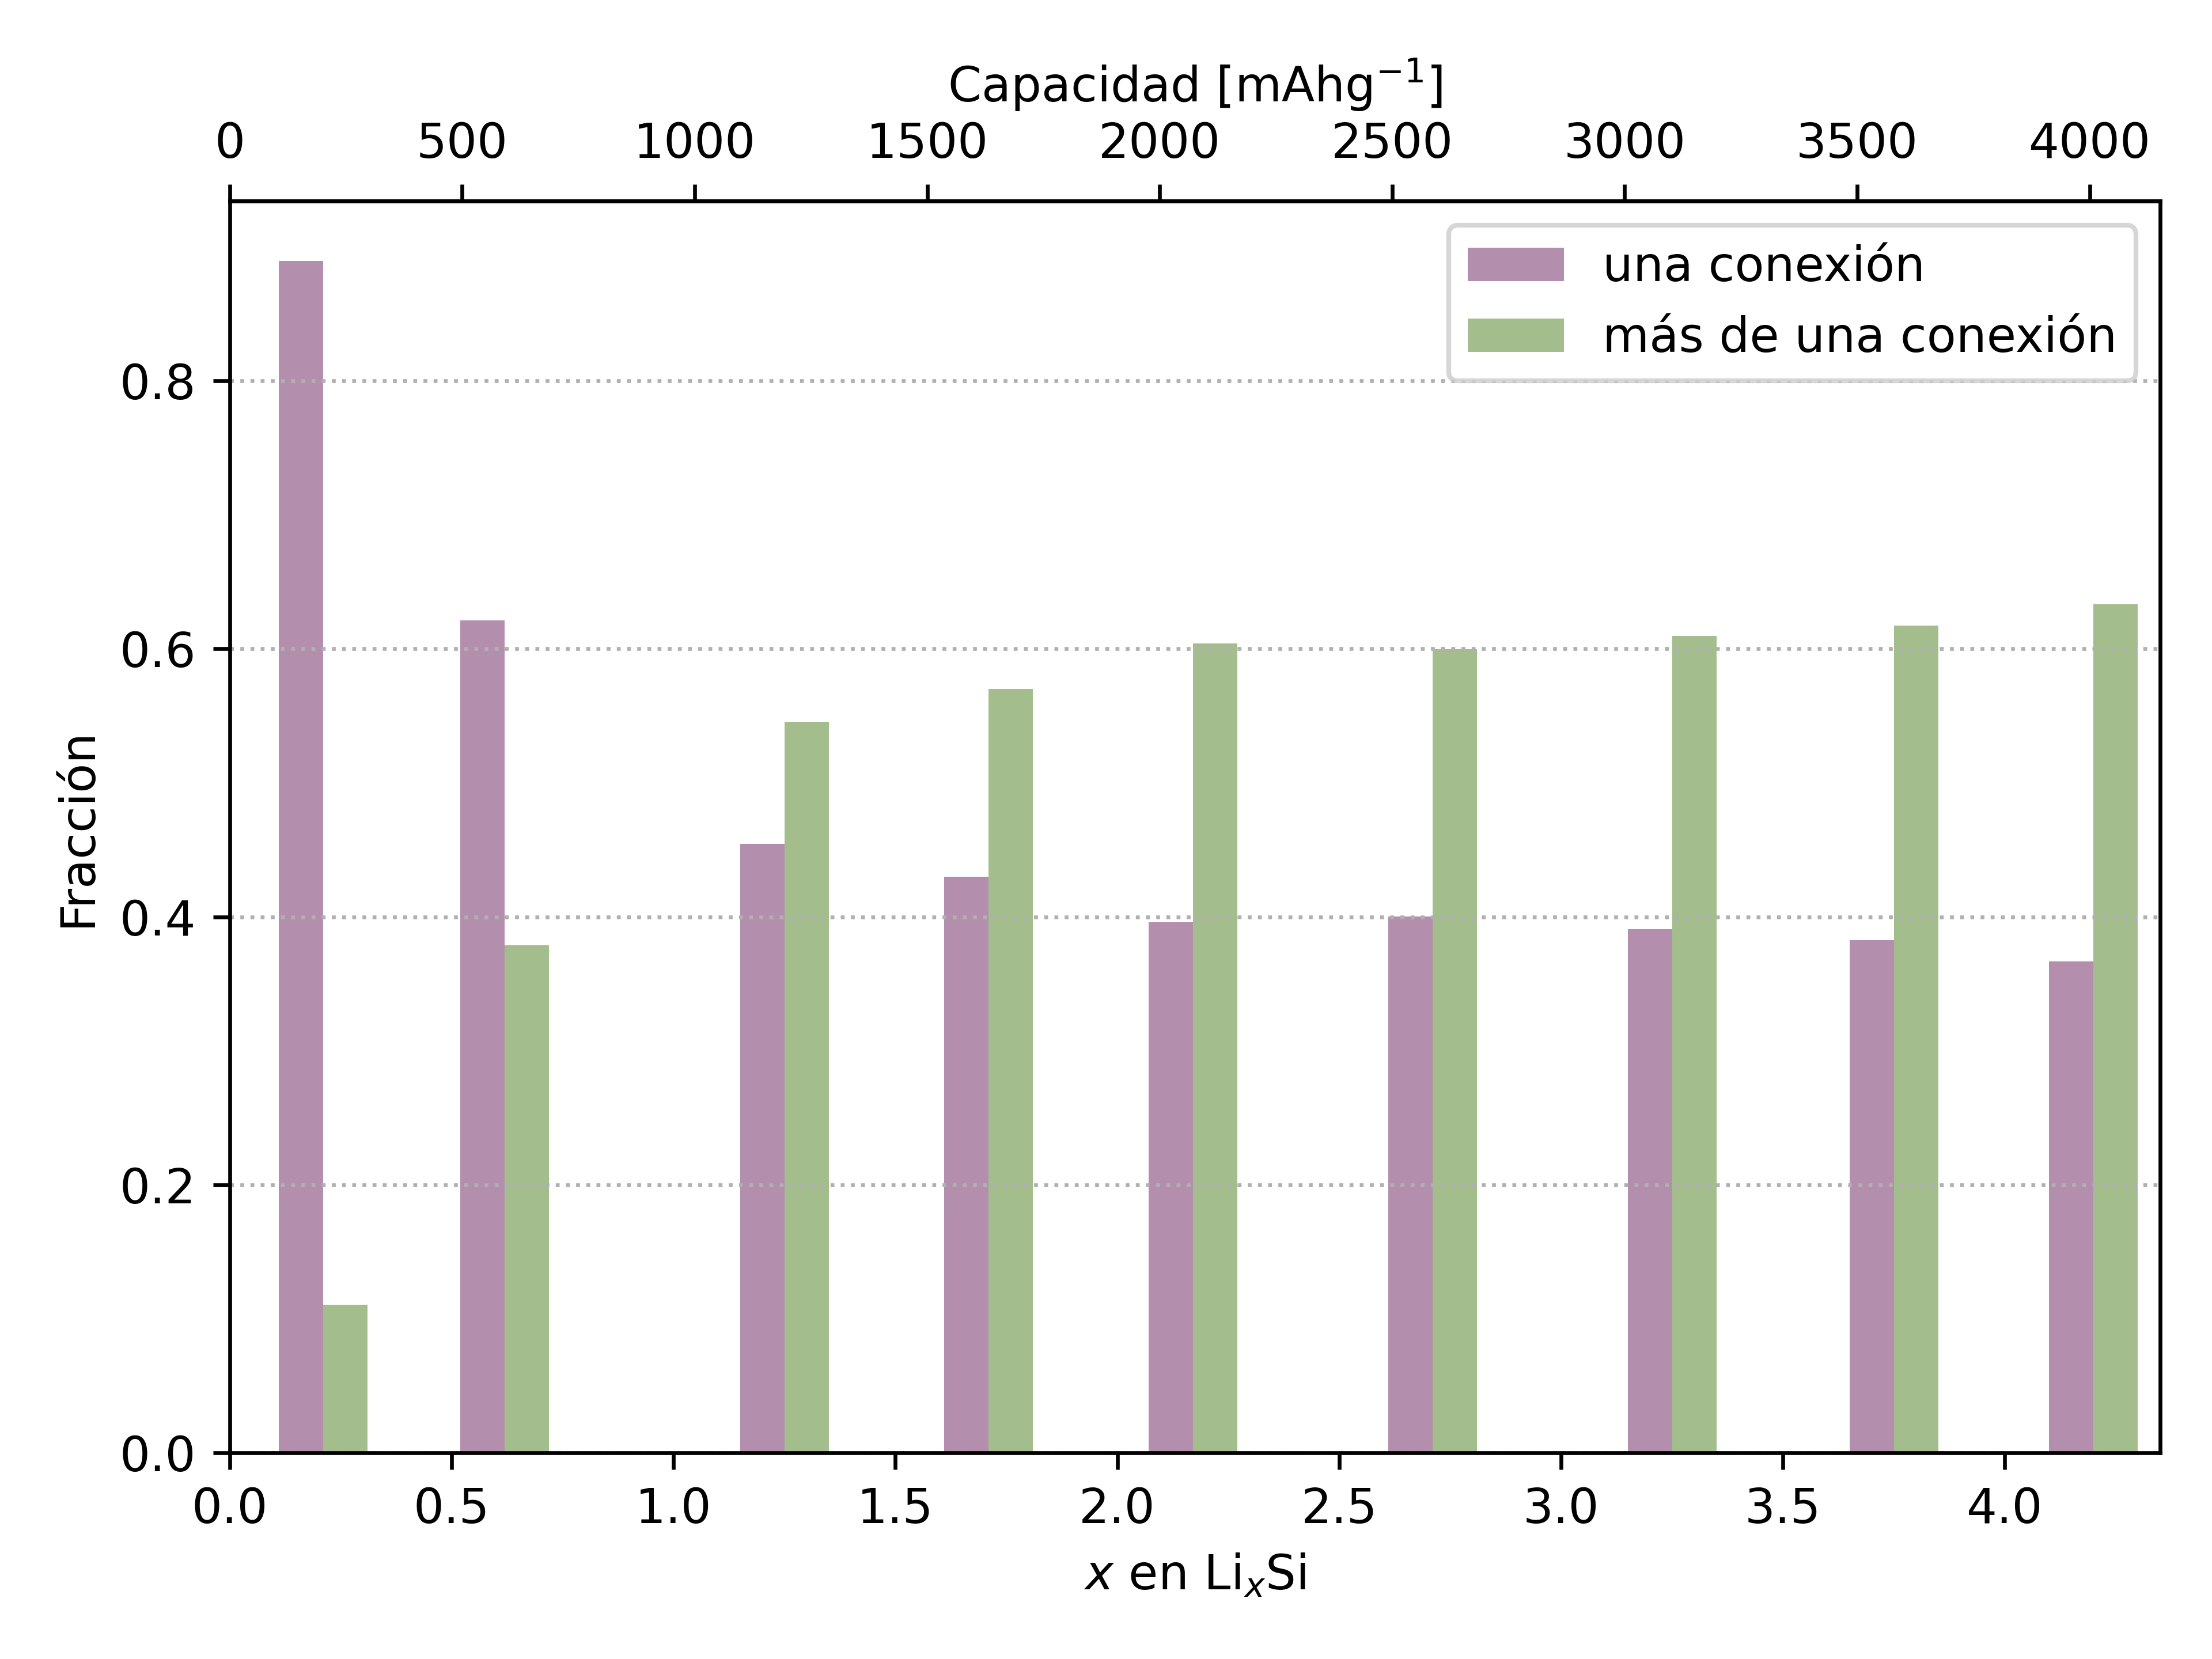
\includegraphics[width=0.8\textwidth]{caracterizacion/interconexiones-areas.png}
    \caption{Evolución con la concentración de la fracción que representa cada
    categoría de interconexiones de Li al área total del segundo pico de la 
    RDF$_{Si-Li}$.}
    \label{fig:interconexiones-areas}
\end{figure}

\subsection{Orden de corto alcance}

El término orden de corto alcance (SRO, de sus siglas en inglés 
\textit{short-range order}) se utiliza para denotar el ordenamiento de los átomos
que rodean a uno específico en una cáscara. Del mismo modo, el término 
\textit{clustering} se ha definido como la tendencia de los átomos similares a 
estar cerca unos de otros. Ambos conceptos se refieren a un orden estructural 
entre átomos vecinos, pero no son necesariamente persistentes a distancias más 
largas. Warren ~\cite{warren69} y Cowley ~\cite{cowley1950} definieron un 
parámetro (WCP) para caracterizar estos tipos de ordenamientos de la siguiente 
manera:
\begin{equation}
    WCP = 1 - \frac{p_{A-B}}{m_B} = 1 - \frac{p_{B-A}}{m_A},
\end{equation}
donde $p_{A-B}(p_{B-A})$ es la probabilidad de tener un átomo de tipo B(A) como
vecino de un átomo de tipo A(B) y $m_B(m_A)$ es la concentración global de átomos
B(A), expresadas en fracciones molares. La igualdad, en ambas definiciones 
posibles del WCP, viene del hecho de que la probabilidad de encontrar a un átomo 
de tipo A como vecino de un átomo de tipo B es igual a la de tener un átomo de 
tipo B como vecino de un átomo de tipo A, esto es $m_A p_{A-B} = m_B p_{B-A}$.

Los valores que se obtienen de utilizar el parámetro WCP en sistemas del tipo
A$_x$B indica una aleatoriedad completa si es igual a cero, preferencia por 
átomos de distinto tipo si $WCP < 0$ y preferencia por átomos del mismo tipo si 
$WCP > 0$. Aunque este parámetro permite un análisis cuantitativo notable, sólo
se define para sistemas cristalinos en los que cada átomo tiene el mismo número
de vecinos. ~\cite{warren69}

A continuación se extiende esta idea para definir un nuevo parámetro, 
$\theta_{A-B}$, que es adecuado para caracterizar estructuras amorfas, de la 
siguiente manera:
\begin{equation}
    \theta_{A-B} = \ln \left( \frac{C_{A-B}}{C_{Bulk}} \right),
\end{equation}
donde A indica la naturaleza del átomo que se considera como central y B el tipo
de átomo que se considera como vecino, equivalente a la definición de WCP. En
este caso, la relación entre la concentración local y la concentración global se 
calcula a partir de la integración de la distribución radial de a pares parcial,
$g_{A-B}(r)$, en una esfera al rededor del átomo central,
\begin{equation}
    \frac{C_{A-B}}{C_{Bulk}} = \frac{1}{V(r_{cut})} \int_0^{r_{cut}} g_{A-B}(r) dV,
\end{equation}
donde $r_{cut}$ y $V(r_{cut})$ son el radio de corte y el volumen de la esfera 
considerada. Ya que en $g_{A-B}(r)$ no hay dependencia angular, $dV$ puede 
escribirse como $4 \pi r^2 dr$. Esta cantidad puede pensarse como la 
concentración promedio dentro de la esfera relativa a la del material 
masivo. Así, de forma análoga al parámetro de WCP, $\theta_{A-B}$ indica 
la tendencia SRO o el \textit{clustering} para cualquier tipo de átomo dado.
Si $\theta$ es positivo, indica una acumulación de átomos relativa al 
\textit{bulk}, mientras que si es negativo indica una disminución. Si es igual a 
cero se tiene una aleatoriedad completa. Este nuevo parámetro también satisface 
la relación $\theta_{A-B} = \theta_{B-A}$ de la misma manera que se discutió para
el parámetro de WCP, ya que por definición $g_{A-B}(r) = g_{B-A}(r)$. Por lo cual 
se tiene que el parámetro $\theta_{A-B}$ da información similar a la que provee 
el WCP, pero además es aplicable a sistemas amorfos.

La figura \ref{fig:sro} muestra la variación del parámetro $\theta$ en función 
de la concentración de Li. Hay tres posibilidades para el análisis de $\theta$ en
sistemas de Li$_x$Si ($\theta_{Li-Li}$, $\theta_{Si-Si}$ y $\theta_{Si-Li}$), ya
que $\theta_{Si-Li} = \theta_{Li-Si}$. Para todos los casos se consideraron los
mismos radios de corte que en los cálculos del número de coordinación, luego del
primer pico de la RDF correspondiente.
\begin{figure}[th]
    \centering
    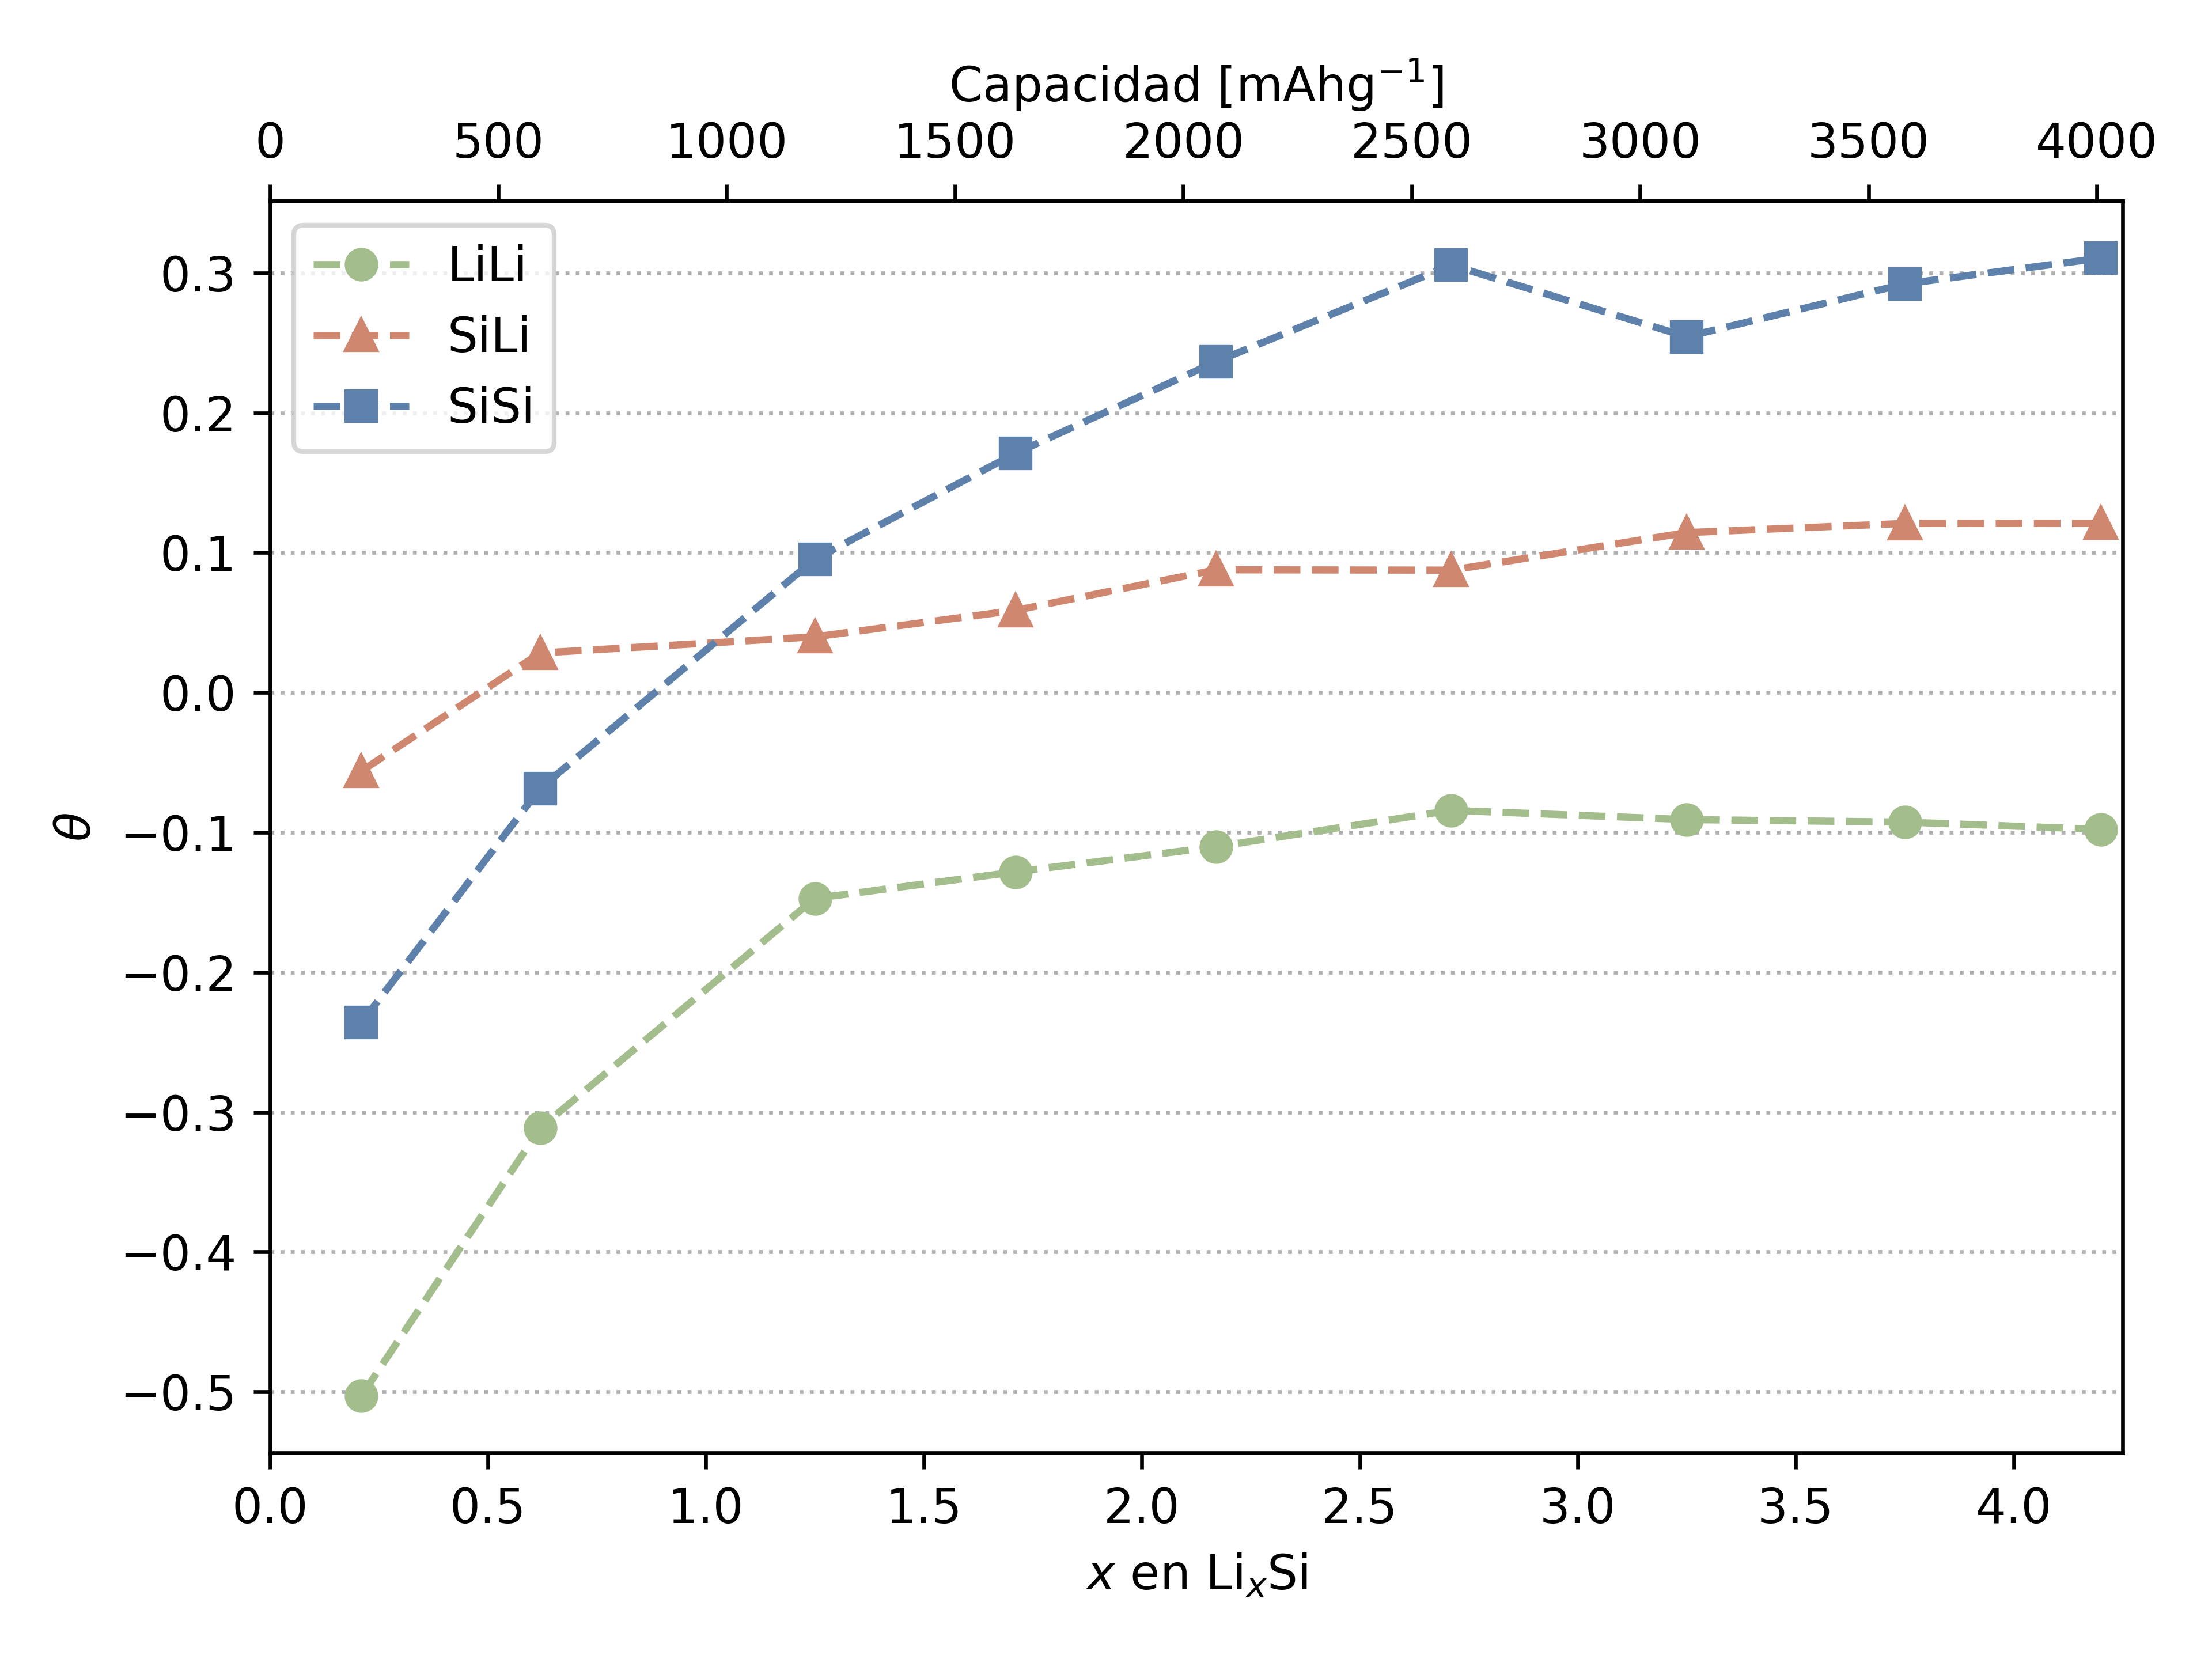
\includegraphics[width=0.8\textwidth]{caracterizacion/sro.png}
    \caption{Parámetros $\theta_{Li-Li}$, $\theta_{Si-Li}$ y $\theta_{Si-Si}$ 
    en función de la concentración de Li. El primer subíndice indica el tipo de
    átomo que se considera como central mientras que el segundo es el vecino. El
    radio de corte se eligió luego del primer pico de la RDF correspondiente.}
    \label{fig:sro}
\end{figure}

Como tendencia general, puede notarse que todos los valores de $\theta$ aumentan
cuando crece la cantidad de litio en el sistema, $x$, y que se estabiliza para 
valores grandes de $x$. Este comportamiento monótono y la disminución en la 
pendiente para concentraciones altas está correlacionado con el comportamiento
presentado en el análisis de los números de coordinación.

En el caso de $\theta_{Si-Si}$, alcanza un valor positivo aproximadamente 
constante para $x > 2.5$, mostrando una correlación fuerte con la presencia de 
cadenas lineales de Si, previamente discutidas y observadas en la figura 
\ref{fig:amorfas}. Aunque la presencia de estas cadenas se puede inferir a partir
de los valores de los CN en $x$ altos, $\theta$ es más sensible al SRO, ya que
está normalizado por la concentración global. Esta propiedad de $\theta$ permite
un análisis más claro incluso si las cadenas están interactuando entre sí, como
es el caso para concentraciones bajas de litio.

$\theta_{Si-Li}$ presenta variaciones pequeñas y un valor positivo para todo 
$x > 0.5$, mostrando una acumulación constante de Li al rededor del Si, o, 
análogamente, una acumulación de Si alrededor del Li. Este comportamiento se le 
puede atribuir a la interacción atractiva fuerte en los pares Si-Li. En el caso de 
$\theta_{Li-Li}$, este parámetro es siempre negativo, lo que indica una 
interacción débil Li-Li y la correspondiente disminución de vecinos Li-Li. Por
último, el parámetro $\theta_{Si-Si}$ tiene un valor negativo para $x < 1.0$, 
sugiriendo que la presencia de concentraciones bajas de litio tiende a separar 
los átomos de silicio entre sí. Sin embargo, $\theta_{Si-Si}$ se vuelve positivo
para $x > 1.0$, implicando una acumulación de vecinos de Si sobre átomos de Si, 
relativo a la concentración global. Esto se debe a la formación de estructuras 
Si-Si. Para $x > 2.5$ puede observarse un valor constante de 
$\theta_{Si-Si} \approx 0.3$, revelando la formación de estructuras estables de 
Si-Si dadas por las cadenas previamente mencionadas.


\section{Conclusiones del capítulo}

Con el fin de emular las estructuras amorfas encontradas en muchos experimentos 
electroquímicos, en este capítulo se generaron estructuras desordenadas de 
aleaciones de Li$_x$Si para varios valores de $x$ utilizando un algoritmo de 
dinámica acelerada y un campo de fuerzas reactivo. La exploración acelerada de 
mínimos locales (AELM) permitió la caracterización de una amplia gama de 
estructuras amorfas. El cambio de volumen de las estructuras litiadas en relación 
con el Si está en concordancia con los resultados experimentales de AFM. Las
energías de las estructuras obtenidas representan bien el comportamiento 
electroquímico de la curva de potencial en función de la concentración de Li. Se 
analizó la función de distribución radial de a pares para los diferentes tipos de 
pares atómicos y se dilucidó la estructura compleja del segundo pico del RDF 
Si-Li mediante un análisis de interconexión de clusters. Además, haciendo un 
análisis de la formación de clústeres en función del radio de corte, se demostró 
que las estructuras amorfas no presentan diferentes enlaces de Si ni átomos de Si 
aislados. En su lugar, se encontró que el sistema se comporta como una red amorfa.
Estudiando los números de coordinación de primeros y segundos vecinos para las 
diferentes concentraciones, se mostró que esta red amorfa mantiene las conexiones 
tetraédricas para bajas concentraciones de Li y que tiende a formar cadenas para 
altas concentraciones de Li. Por último, la definición de un nuevo parámetro 
permitió determinar el orden de corto alcance de las estructuras amorfas, definido
por interacciones débiles Li-Li y fuertes Li-Si y Si-Si. El método propuesto AELM 
resulta ser un método rápido y eficaz para obtener mínimos energéticamente 
relevantes. Se hizo una analogía con el templado simulado múltiple. Un análisis 
detallado de la eficiencia de AELM en comparación con otros métodos eficientes 
como el templado simulado múltiple o los métodos de Monte Carlo es una motivación 
para trabajos futuros.



% Apéndices
% \appendix
% \chapter[Apéndice X]{Apéndice X}
% \input{src/apendicex.tex}

\bibliographystyle{ieeetr}
\bibliography{citas.bib}

\end{document}
